\documentclass[12pt]{article}
\usepackage[utf8]{inputenc}

%----------Packages----------
\usepackage{fullpage}  %%smaller margins
\usepackage{amsmath,amssymb,amsthm}
\usepackage[mathcal]{eucal}
\usepackage{mathpazo}
\usepackage{graphicx}
\usepackage{subcaption}
\usepackage[numbers,sort&compress]{natbib}
\usepackage{hyperref}  %%load last

\graphicspath{{figures/}}
\let\emptyset\varnothing

%----------Commands----------
\def\ZZ{\mathbb{Z}}
\def\QQ{\mathbb{Q}}
\def\PP{\mathbb{P}}
\def\NN{\mathbb{N}}
\def\OO{\mathcal{O}}
\def\AA{\mathbb{A}}
\def\BB{\mathbb{B}}
\def\II{\mathbb{I}}
\def\FF{\mathbb{F}}
\def\LL{\mathbb{L}}
\def\RR{\mathbb{R}}
\def\CC{\mathbb{C}}
\def\GG{\mathbb{G}}

%----------Theorems----------
\newtheorem{theorem}{Theorem}[section]
\newtheorem{proposition}[theorem]{Proposition}
\newtheorem{claim}[theorem]{Claim}
\newtheorem{lemma}[theorem]{Lemma}
\newtheorem{example}[theorem]{Example}
\newtheorem{solution}[theorem]{Solution}
\newtheorem{corollary}[theorem]{Corollary}
\theoremstyle{definition}
\newtheorem{definition}[theorem]{Definition}
\newtheorem*{definition*}{Definition}

\title{
    {Topological Surface Codes on Exactly Solvable Lattice Models}\\
    \vspace{10pt}
    {
\includegraphics[scale=0.3]{kcl.png}}
}

\author{
    \textbf{Flavio D. Gualtieri}\\
    \vspace{20pt}
    King's College London
    Department of Mathematics\\
    \vspace{20pt}
    This dissertation is submitted for the degree of\\
    \emph{Master of Science in Theoretical Physics}
}

\date{
    \vspace*{\fill}
    November 2024
}

\begin{document}

\maketitle

\tableofcontents

\section{Introduction}
Quantum error correction is an indispensable component of fault-tolerant quantum computation, addressing the major challenge posed by decoherence and local noise. Among the various paradigms for quantum error correction, topological codes stand out for their intrinsic ability to protect quantum information from local errors by encoding it in global degrees of freedom and leveraging the exotic topological properties of the underlying surface \cite{anintro}. These codes are defined on lattice models, and notable examples include the toric code and color code, each offering unique approaches to protecting quantum information.\newline

It is particularly instructive to study toric codes because they illustrate the important role of algebraic topology in enabling surface codes to encode quantum information in non-local degrees of freedom, thereby ensuring resilience to local perturbations. This resilience arises from the lattice's topological structure, which guarantees that logical operations correspond to global transformations immune to localized noise. By examining the stabilizer constraints, logical operators, and topological invariants, our study of the toric code provides a framework for understanding the paradigm of topological surface codes and motivates exploring more complex models that extend these principles to higher dimensions and alternative lattice geometries.\newline

Building on this framework, we turn to color codes and their capacity to implement logical gates beyond the Clifford group. Specifically, we investigate methods for constructing logical operators in both toric and color codes, with an emphasis on achieving fault tolerance through transversal operations. By leveraging the unique topological properties of these models, we identify strategies for constructing higher-dimensional quantum gates.\newline

Through this paper, we aim to deepen the understanding of logical operator construction in topological codes and provide a pathway for implementing transversal gates. Our analysis highlights the interplay between lattice topology, operator design, and the stabilizer formalism, contributing to the broader effort of realizing scalable quantum technologies.\newline

Before delving into this work, we turn the reader's attention to the Appendix, which outlines essential notions in algebraic topology and the abstract structure of lattice models. This foundational material provides the necessary framework to understand the topological features of the codes discussed here. Concepts such as homology, cohomology, and the classification of boundary operators are introduced to equip the reader with the tools required for the subsequent analysis, offering a self-contained presentation accessible to both physicists and mathematicians interested in topological quantum computation.
\newpage
\section{Two Dimensional Toric Codes}
The toric code is a foundational model for quantum error correction, introduced by Alexei Kitaev in 1997 \cite{kitaev1997}. It illustrates how quantum information can be stored and manipulated in a two-dimensional lattice with periodic boundary conditions. This section introduces the basic structure and mathematical framework of the toric code, including its stabilizer formalism, Hamiltonian, and its topological features that enable fault-tolerant quantum computation.

\subsection{Defining the Toric Code}
In order to construct the toric code code we require two ingredients:
    \begin{enumerate}
        \item A $2$-dimensional $k\times k$ square lattice $\mathcal{L}$ equipped with periodic boundary conditions \footnote{In this case, periodic boundary conditions imply that opposite edges on the lattice are 'attached'} such that it discretizes a two-dimensional torus
        \item Vectors belonging to a $2$-dimensional Hilbert space $\mathcal{H}_2$ are assigned to each edge of $\mathcal{L}$, with basis $\{|g\rangle\mid g\in \mathbb{Z}_2\}$. These vectors are interpreted as quantum bits (\emph{qubits})
    \end{enumerate}
There are $N = 2k^2$ edges on the lattice (due to the periodic boundary conditions, each plaquette of the lattice has two independent edges), and each edge of $\mathcal{L}$ is associated to a Hilbert space $\mathcal{H}_2$; it follows that the total Hilbert space of the system $\mathcal{H}_{TC}$ is:
    \begin{align}
        \mathcal{H}_{TC} = \mathcal{H}^{\otimes N}_2.
    \end{align}
It is clear that $\text{dim}\mathcal{H}_{TC} = 2^{N}$. We will use $\{|0\rangle,|1\rangle\}$ as a basis for the $\mathcal{H}_2$ Hilbert spaces on each edge. $V$, $E$, and $P$ will be used to denote the sets of vertices, edges, and plaquettes in $\mathcal{L}$, respectively. The state of the system is therefore described by:
    \begin{align}
        |\psi_{TC}\rangle :=\bigotimes_{e\in E}|c_e\rangle,\enspace\enspace |c_e\rangle\in \{|0\rangle,|1\rangle\}.
    \end{align}
In accordance with the conventions overwhelmingly established in the literature, product notation ($\prod$) will be used for Pauli operators, and tensor product notation ($\otimes$) will be used in all other cases.\newpage

\subsection{Stabilizer Formalism and Hamiltonian}
As the lattice $\mathcal{L}$ is composed of vertices and plaquettes, we may define the following operators in terms of the Pauli spin matrices $\sigma^x$ and $\sigma^z$:
    \begin{align}
        \{A_v\}_{v\in V} =\prod_{e|v\in\partial_1e}\sigma^x_e,\enspace\enspace\enspace \{B_p\}_{p\in P} =\prod_{e\in\partial_2p}\sigma^z_e,
    \end{align}
for $e\in E$. In what is perhaps an abuse of notation, we understand $\partial_1e$ and $\partial_2p$ as sets. $A_v$ and $B_p$ are commonly referred to as \emph{vertex} and \emph{plaquette} stabilizer operators, respectively, and generate the \emph{stabilizer group} of the toric code:
    \begin{align}
        \mathcal{S}_{TC} := \langle\{A_v\}_{v\in V},\{B_p\}_{p\in P}\rangle.
    \end{align}
The vertex operator applies $\sigma^x$ to all edges incident on a certain vertex, and the plaquette operator applies $\sigma^z$ to all edges surrounding a plaquette. Since the Pauli matrices are Hermitian, it follows that $A_v$ and $B_p$ are also Hermitian \cite{kitaev1997}. 
    \begin{figure}[h]
    \centering
    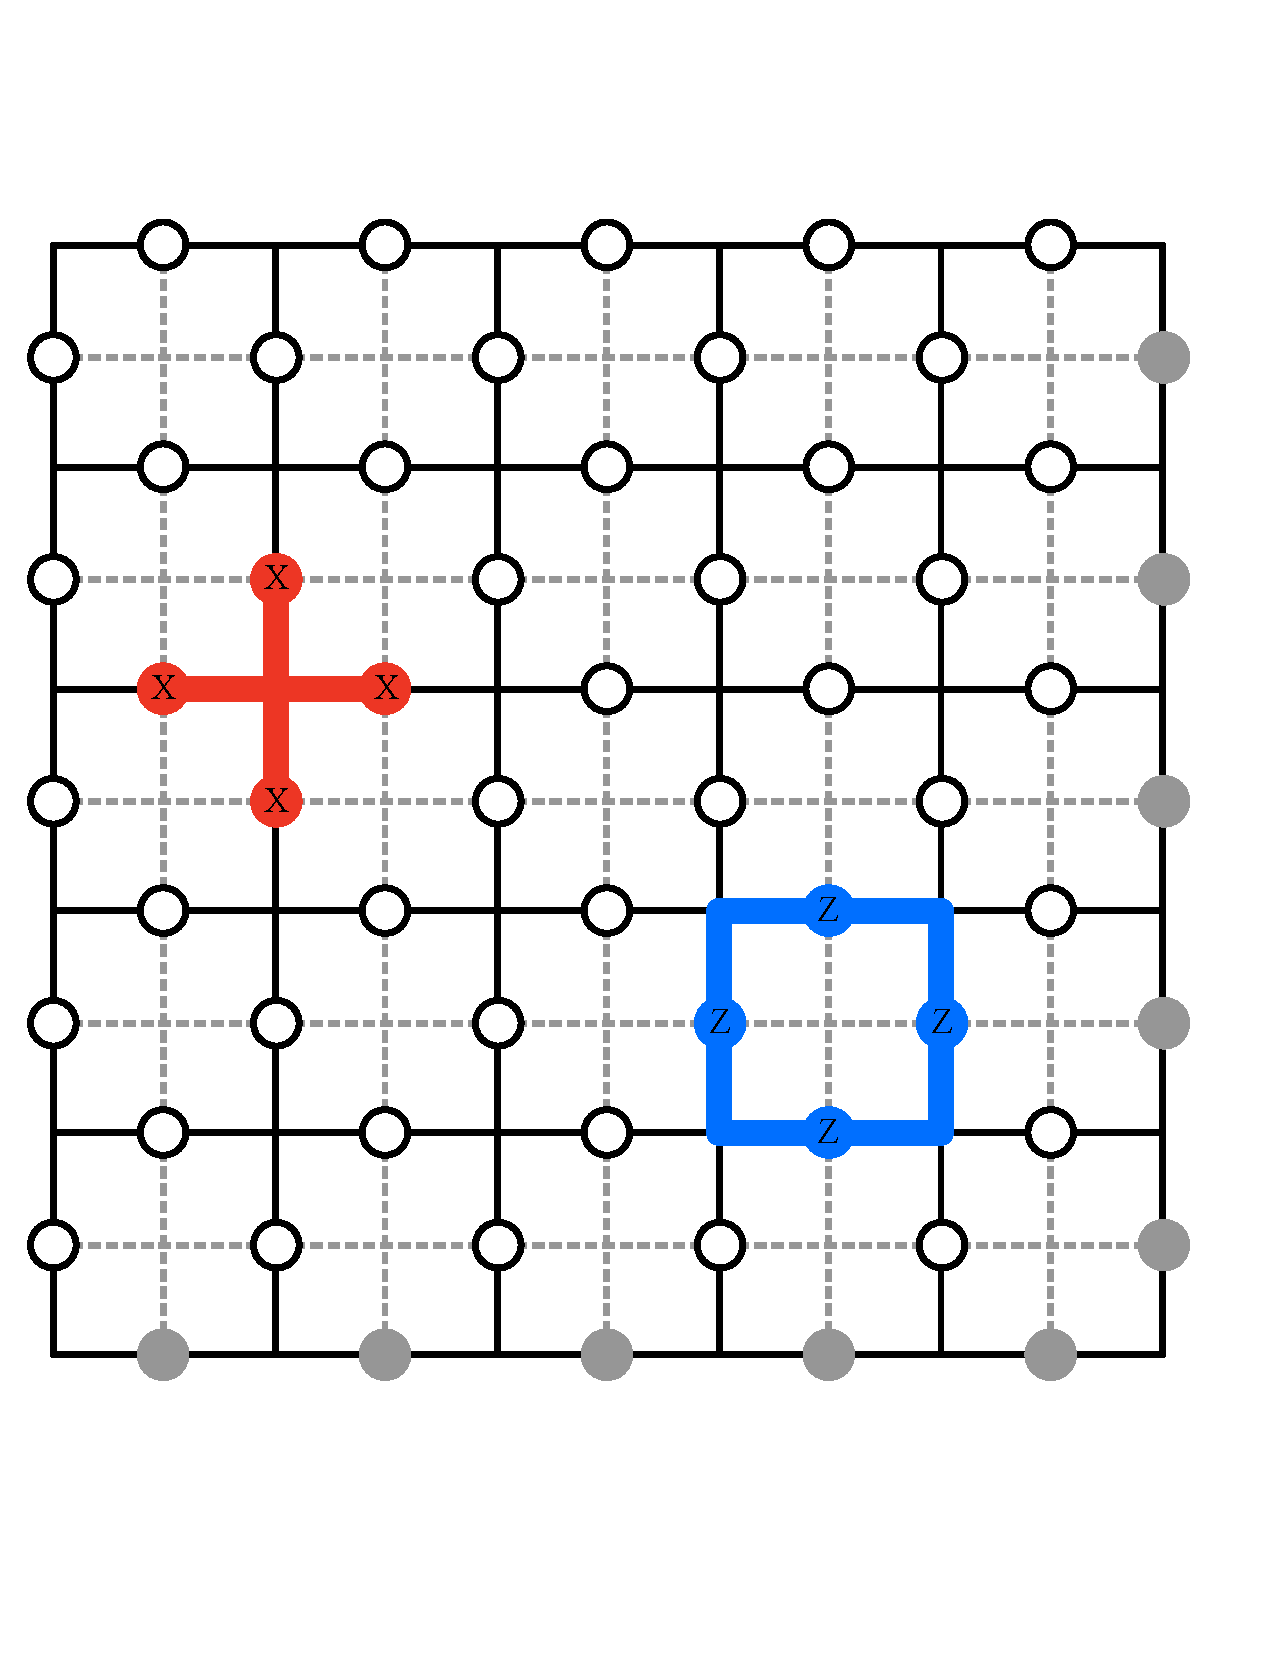
\includegraphics[width=0.4\textwidth]{new_stabs.pdf}
    \caption{ Example of a plaquette operators (blue) and a vertex operator (red). Moving forward, red-filled edges will always represent $\sigma^x$ operators, and blue-filled edges will always represent $\sigma^z$ operators.}
    \label{fig:x stabilizer operators}
    \end{figure}
        
The toric code Hamiltonian $H_{TC}$ captures the essential topological properties of the system and is defined in terms of the stabilizer operators \cite{kitaev1997,ellison2022,gaspari2020}:
    \begin{align}
        H_{TC} = -\sum_{v\in V}A_v-\sum_{p\in P}B_p.
    \end{align}
It is important to note that when we define an operator to be a Hamiltonian, such an operator must have the ability to measure the total energy of the system in question.\newline

Shifting our focus back to the stabilizer operators, there are some important properties of $A_v$ and $B_p$ to consider. For any given pair of states $|\psi\rangle,|\psi^{'}\rangle\in\mathcal{H}_{TC}$, we have that for all $v,v'\in V$, and all $p,p'\in P$ \cite{kitaev1997}:
    \begin{enumerate}
        \item $A_v|\psi\rangle = \pm1|\psi\rangle$ and $B_p|\psi\rangle = \pm1|\psi\rangle$
            \begin{proof}
                We have:
                    \begin{align}
                        A^2_v = \prod_{e|v\in\partial_1e}(\sigma^x_e)^2 = \II,\enspace\enspace\enspace B^2_p = \prod_{e\in\partial_2p}(\sigma^z_e)^2 = \II,
                    \end{align}
                where we have used the well-known property $(\sigma^x)^2 = (\sigma^z)^2 = \II$. Since $A_v$ and $B_p$ are Hermitian, they are diagonalizable and their eigenvalues are real. Let $|\xi\rangle$ be an eigenstate of $A_v$ with eigenvalue $\lambda\in\RR$. It follows:
                    \begin{align}
                        A^2_v(|\xi\rangle)^2 &= \lambda^2(|\xi\rangle)^2\\
                        (|\xi\rangle)^2 &= \lambda^2(|\xi\rangle)^2\\
                        \II &= \lambda^2.
                    \end{align}
                Since $\lambda\in\RR$, then $\lambda = \pm1$. An equivalent argument can be made for $B_p$.
            \end{proof}
        \item $\prod_{v\in V}A_v = \prod_{p\in P}B_p = \II$
            \begin{proof}
                Let $p_0\in P$ with $\partial_2p := \{e_1,e_2,e_3,e_4\}$ for $e_1,e_2,e_3,e_4\in E$. We have:
                    \begin{align}
                        B_{p_0} &= \sigma^z_{e_1}\sigma^z_{e_2}\sigma^z_{e_3}\sigma^z_{e_4}\\
                        &= \II,
                    \end{align}
                where we have once again used the property $(\sigma^z)^2 = \II$. An equivalent argument can be made for $A_v$.
            \end{proof}
        \item $[A_v,A^{'}_v] = [B_p,B^{'}_p] = 0$
            \begin{proof}
                This statement is trivial, as $[\sigma^x,\sigma^x] = [\sigma^z,\sigma^z] = 0$.
            \end{proof}\newpage
                \begin{figure}[h]
                \centering
                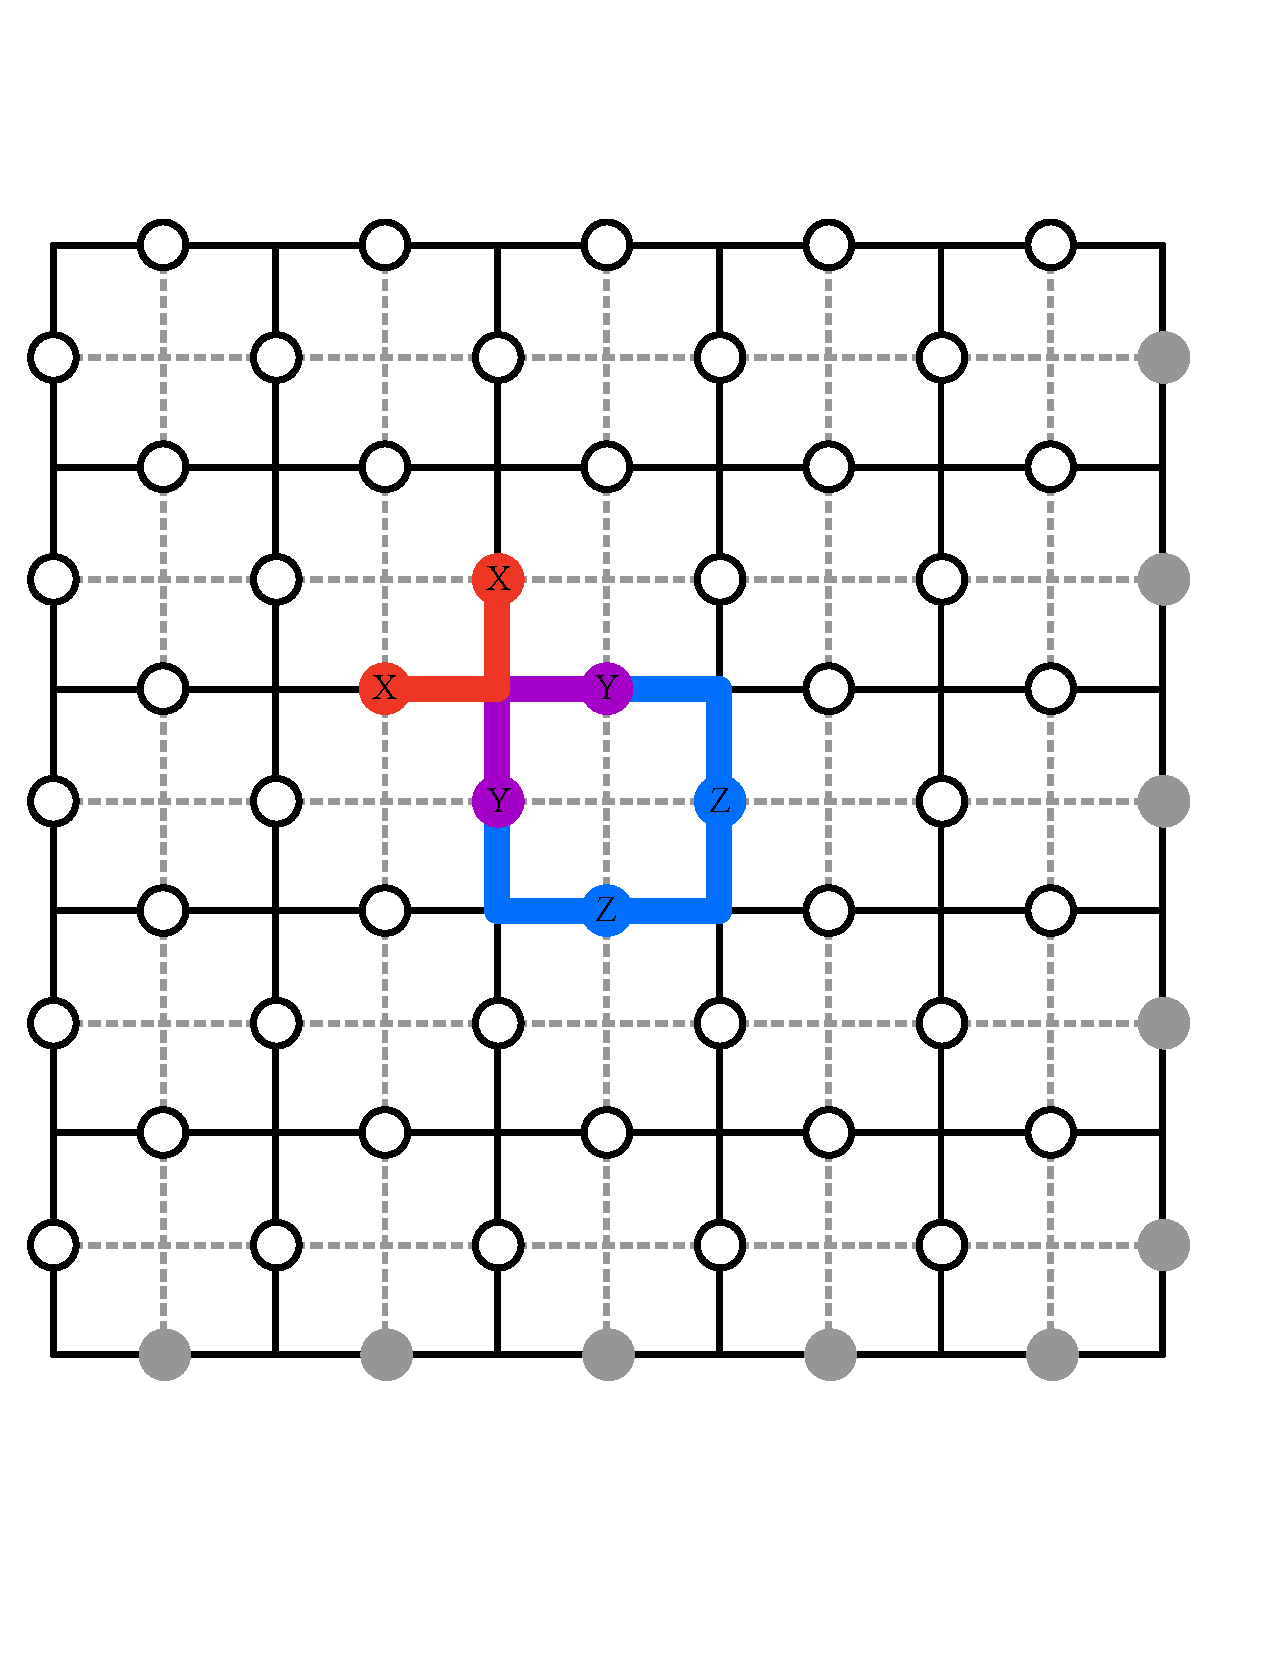
\includegraphics[width=0.4\textwidth]{overlap.pdf}
                \caption{When vertex and plaquette operators overlap, they do so over two edges. Purple edges represent $\sigma^y$ operators, which occur when $\sigma^z$ and $\sigma^x$ coincide on the same edge.}
                \label{fig:x stabilizer overlap}
                \end{figure}
        \item $[A_v,B_p] = 0$
            \begin{proof}
                This statement holds trivially when the stabilizer operators do not coincide on any edges, as spins on separate edges commute automatically. In the case that $A_v$ and $B_p$ do coincide, by construction they must necessarily do so over two edges, see Figure~\ref{fig:x stabilizer overlap}. Let $p_0\in P$ with $\partial_2p_0 := \{e_1,e_2,e_3,e_4\}$ for $e_1,e_2,e_3,e_4\in E$. Consider a vertex operator $A_{v_0}$ for $v_0\in V$ that acts on two of the edges in $\partial_2p_0$. Without loss of generality, we will take $v_0\in\partial_1e_1\cap\partial_1e_2$, implying that $B_{p_0}$ and $A_{v_0}$ overlap on edges $e_1$ and $e_2$. We label the remaining two edges that $A_{v_0}$ acts on as $e_A$ and $e_B$. For some state $|\xi\rangle\in\mathcal{H}_{TC}$ we have:
                    \begin{align}
                        A_{v_0}B_{p_0}|\xi\rangle &= (\sigma^x_{e_A}\sigma^x_{e_B}\sigma^x_{e_2}\sigma^x_{e_1})(\sigma^z_{e_1}\sigma^z_{e_2}\sigma^z_{e_3}\sigma^z_{e_4})|\xi\rangle\\
                        &= -(\sigma^x_{e_A}\sigma^x_{e_B}\sigma^x_{e_2})\sigma^z_{e_1}\sigma^x_{e_1}(\sigma^z_{e_2}\sigma^z_{e_3}\sigma^z_{e_4})|\xi\rangle\\
                        &= -\sigma^z_{e_1}(\sigma^x_{e_A}\sigma^x_{e_B}\sigma^x_{e_2})(\sigma^z_{e_2}\sigma^z_{e_3}\sigma^z_{e_4})\sigma^x_{e_1}|\xi\rangle\\
                        &= \sigma^z_{e_1}(\sigma^x_{e_A}\sigma^x_{e_B})\sigma^z_{e_2}\sigma^x_{e_2}(\sigma^z_{e_3}\sigma^z_{e_4})\sigma^x_{e_1}|\xi\rangle\\
                        &= (\sigma^z_{e_1}\sigma^z_{e_2}\sigma^z_{e_3}\sigma^z_{e_4})(\sigma^x_{e_A}\sigma^x_{e_B}\sigma^x_{e_2}\sigma^x_{e_1})|\xi\rangle\\
                        &= B_{p_0}A_{v_0}|\xi\rangle.
                    \end{align}
                Therefore $[A_{v_0},B_{p_0}] = 0$. Note that in $(13)$ and $(15)$ we used the property $\{\sigma^x_e,\sigma^z_{e'}\} = 0$ for $e = e'$, and throughout our reasoning we applied the fact $[\sigma^x_e,\sigma^z_{e'}] = 0$ if $e\neq e'$.
            \end{proof}\newpage
        \item $[A_v,H_{TC}] = [B_p,H_{TC}] = 0$
            \begin{proof}
                Using properties $3$ and $4$, we may compute this commutator directly. Let $v_0\in V$:
                    \begin{align}
                        [A_{v_0},H_{TC}] &= [A_{v_0},-\sum_{v\in V}A_v-\sum_{p\in P}B_p]\\
                        &= -[A_{v_0},\sum_{v\in V}A_v]-[A_{v_0},\sum_{p\in P}B_p]\\
                        &= 0.
                    \end{align}
                An equivalent argument can be made for $\{B_{p}\}_{p\in P}$.
            \end{proof}
    \end{enumerate}
As a result of the fourth property, all the $A_v$ and $B_p$ operators can be simultaneously diagonalized, and the ground state of the system will be a simultaneous eigenstate of these operators. Therefore the states in $\mathcal{H}_{TC}$ can be labeled by the eigenvalues of the stabilizers.\newline

Stabilizer generators are not all independent. From property $2$, it follows that there are $|V|+|P|-2$ independent generators, where $|V|$ and $|P|$ denote the number of vertices and plaquettes in $\mathcal{L}$, respectively. Therefore, the number of encoded qubits in the code is $|E|-|V|+|P|-2 = 2-\chi = 2g$ \cite{anintro}, where $\chi$ and $g$ are the Euler characteristic and genus of the surface, respectively (refer to Appendix $A$). For the torus $g = 1$, so this framework encodes two qubits.

\subsection{Ground State Degeneracy}
\subsubsection{The Protected Subspace}
We now have the tools to study the ground state of the system. In order to do this, we must look to minimize the energy of $H_{TC}$. Logically, this must be done by maximizing the stabilizer terms \cite{bravyi1998}. We begin by defining the \emph{protected subspace} $\mathcal{H_L} \subseteq \mathcal{H}_{TC}$. This is the subspace that is stabilized by all $A_v$ and $B_p$. Formally:
    \begin{align}
        \mathcal{H_L} := \{|\xi\rangle\in\mathcal{H}_{TC}\mid A_v|\xi\rangle = B_p|\xi\rangle = |\xi\rangle\enspace\forall\enspace v\in V, p\in P\}.
    \end{align}
The dimensionality of $\mathcal{H_L}$ can be calculated by considering the aforementioned property 2, from which we have seen that that on a $k\times k$ lattice the number of independent $A_v$ operators is $k^2-1$, and the number of independent $B_p$ operators is also $k^2-1$. Therefore, the total number of independent stabilizer operators is $M = 2k^2-2$. Recall that the number of spins on the lattice is $N = 2k^2$. The dimensionality of the protected subspace is then given by \cite{kitaev1997, kitaev2009, ellison2022}:
    \begin{align}
        \dim\mathcal{H_L} = 2^{N - M} = 2^{2k^2 - (2k^2 - 2)} = 4.
    \end{align}
This $4$-dimensional protected subspace is essential to the surface code's ability to store and protect quantum information. We will see that this dimensionality is a result of the lattice's topological structure, and the robustness of the code arises from this topological structure, as logical qubits are stored in non-local degrees of freedom, making the code resilient to local errors.

\subsubsection{Topological Numbers and Degeneracy}
We seek to develop a more sophisticated understanding of the ground state, especially its relationship to the surface's topology. To do so, it is constructive to consider the conditions defined by each stabilizer individually. Let us first restrict our attention to the constraint imposed by the plaquette operators, which defines the subspace:
    \begin{align}
        \mathcal{H}_B := \{|\psi\rangle\in\mathcal{H}_{TC}\mid B_p|\psi\rangle = |\psi\rangle\enspace\forall\enspace p\in P\}.
    \end{align} 
It is worth noting that $\mathcal{H_L}\subseteq\mathcal{H}_B\subseteq\mathcal{H}_{TC}$. Logically, we will work in the $\sigma^z$-product basis and label states in this subspace by the eigenvalues of $B_p$. Recall that for all $e\in E$, we have $|c_e\rangle\in\mathcal{H}_2 := \{|0\rangle,|1\rangle\}$. In this basis, we assign:
    \begin{align}
        \sigma^z|0\rangle &= |0\rangle\\
        \sigma^z|1\rangle &= -|1\rangle.
    \end{align}
For simplicity, we may assign a spin label $s_e$ to each edge:
    \begin{align}
        s_e = \begin{cases}
            0 & \mbox{if}\enspace |c_e\rangle = |0\rangle\\
            1 & \mbox{if}\enspace |c_e\rangle = |1\rangle
        \end{cases}
    \end{align}
Using these tools, we may define the \emph{parity} $\nu_p(\xi)$ of a plaquette $p\in P$ for a state $|\xi\rangle\in\mathcal{H}_{TC}$:
    \begin{align}
        \nu_p(\xi) = \sum_{e\in\partial_2p}s_e\enspace(\text{mod}\enspace2).
    \end{align}
It follows that we can make the following claim:
    \begin{claim}
        $|\psi\rangle\in\mathcal{H}_B\enspace\text{if and only if}\enspace \nu_p(\psi) = 0\enspace(\text{mod}\enspace2)\enspace\forall\enspace p\in P$
    \end{claim}
    \begin{proof}
        $(\rightarrow)$ Suppose $|\psi\rangle\in\mathcal{H}_B$, then $B_p|\psi\rangle = |\psi\rangle\enspace\forall\enspace p\in P$. Let $p_0\in P$; there are three possible cases:
            \begin{enumerate}
                \item $|c_{e}\rangle = |0\rangle\enspace\forall\enspace e\in\partial_2p_0$
                \item $|c_{e}\rangle = |1\rangle\enspace\forall\enspace e\in\partial_2p_0$
                \item $|c_{e}\rangle = |0\rangle$ for two $e\in\partial_2p_0$ and $|c_{e}\rangle = |1\rangle$ for the remaining two $e\in\partial_2p_0$
            \end{enumerate}
        One can easily check that in each case $\nu_{p_0}(\psi) = 0\enspace(\text{mod}\enspace2)$.\newline\newline
        $(\leftarrow)$ Let $|\xi\rangle\in\mathcal{H}_{TC}$. Suppose $\nu_p(\xi) = 0\enspace(\text{mod}\enspace2)\enspace\forall\enspace p \in P$, then for some $p_0\in P$ there are once again three possible cases:
            \begin{enumerate}
                \item $|c_{e}\rangle = |0\rangle\enspace\forall\enspace e\in\partial_2p_0$
                \item $|c_{e}\rangle = |1\rangle\enspace\forall\enspace e\in\partial_2p_0$
                \item $|c_{e}\rangle = |0\rangle$ for two $e\in\partial_2p_0$ and $|c_{e}\rangle = |1\rangle$ for the remaining two $e\in\partial_2p_0$
            \end{enumerate}
        Since these are the exact same cases presented in the forward proof, it follows that $B_p|\xi\rangle = |\xi\rangle$, and therefore $|\xi\rangle\in\mathcal{H}_B$.
    \end{proof}
We can therefore redefine $\mathcal{H}_B$:
    \begin{align}
        \mathcal{H}_B := \{|\psi\rangle\in\mathcal{H}_{TC}\mid\nu_p(\psi) = 0\enspace (\text{mod}\enspace2)\enspace\forall\enspace p\in P\}.
    \end{align}
    \begin{figure}[h]
        \centering
        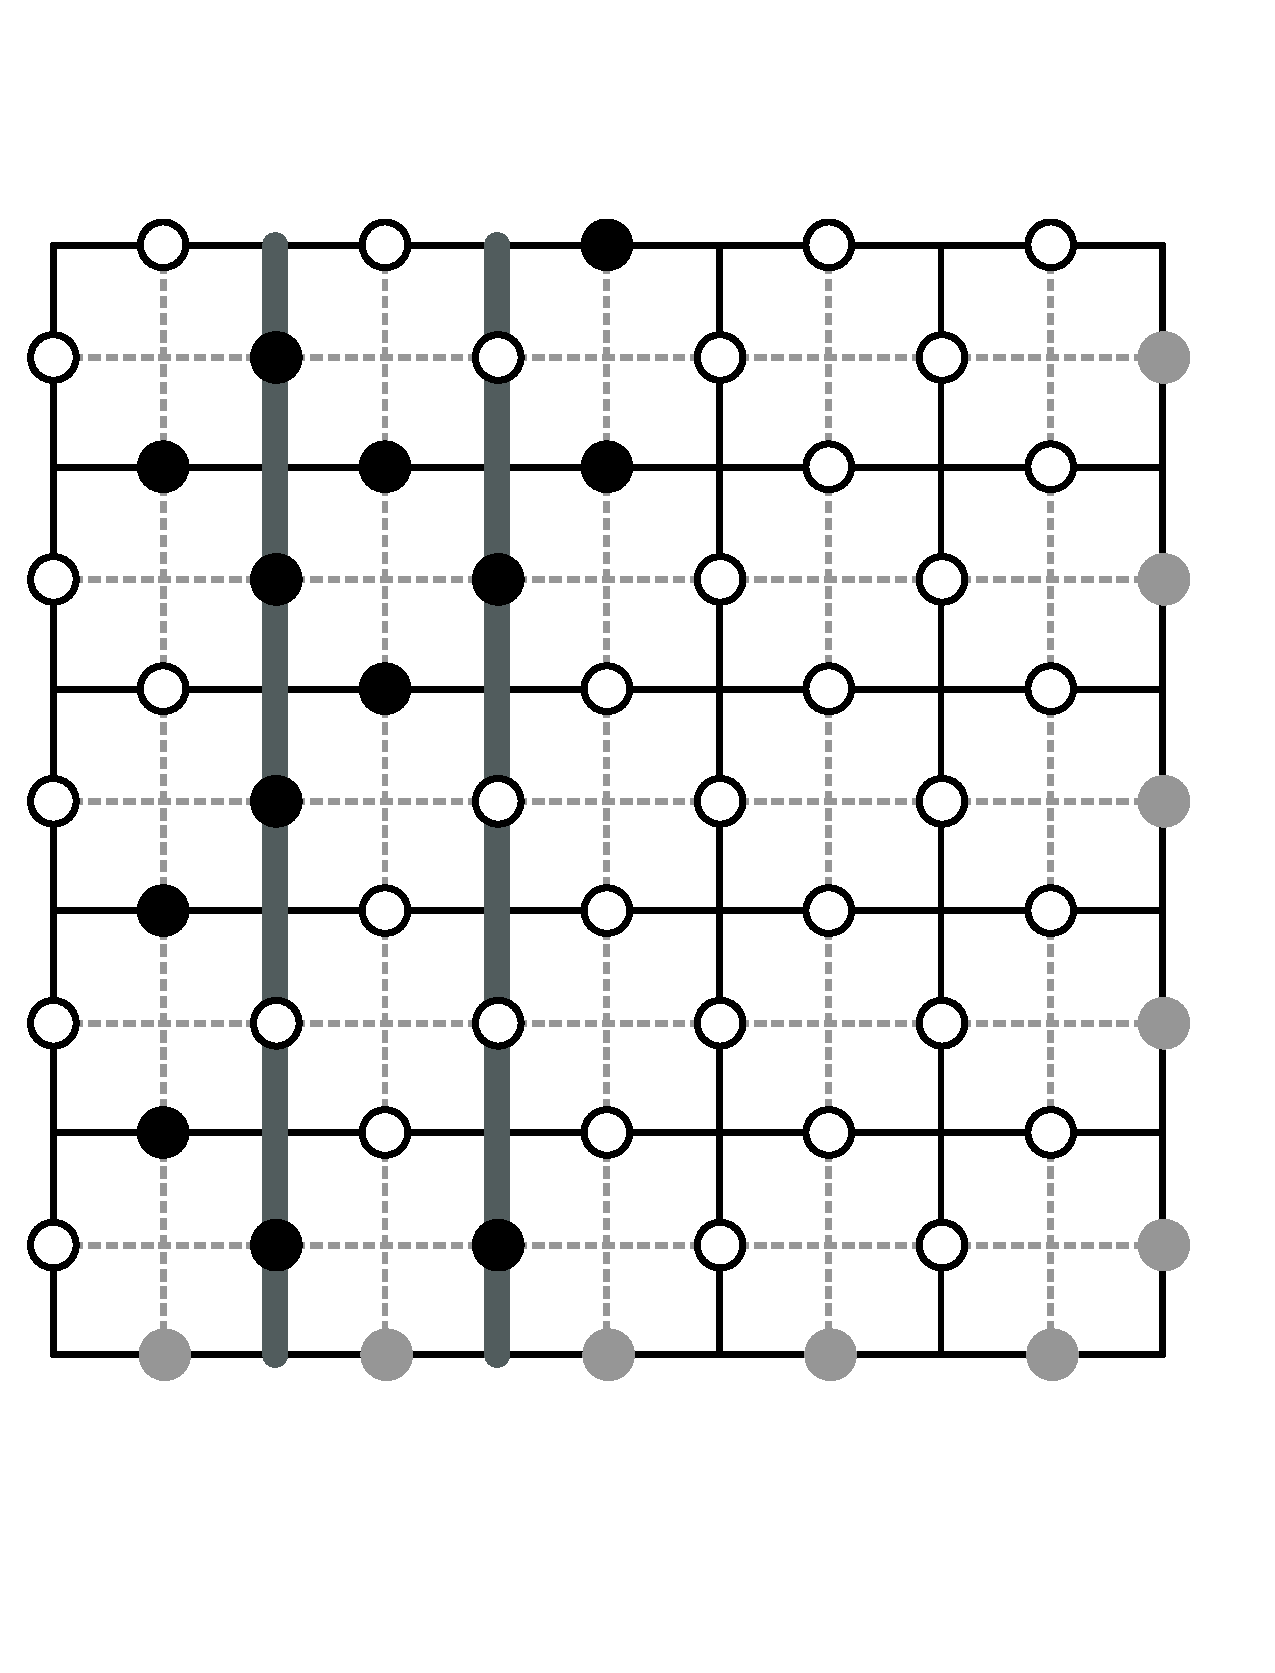
\includegraphics[width=0.4\textwidth]{parity.pdf}
        \caption{On a ground state configuration of $\mathcal{H}_B$ (black edges represent qubits in the $|1\rangle$ state) one finds that the parities of adjacent elements of $H^v_1$ are equal}
        \label{fig:x parity of columns}
    \end{figure}

This notion of plaquette parity has more profound topological implications. Consider the elements of the first homology group of the torus, which on $\mathcal{L}$ can be interpreted as non-contractible $1$-chains that wrap around the lattice in each direction (vertically and horizontally). For simplicity, we will use $H^v_1 := \{c_i\}_{i\in\{1,...,k\}}$ to denote the set of vertical non-contractible $1$-chains, where $i$ indexes over the $k$ columns of $\mathcal{L}$. For $|\psi\rangle\in\mathcal{H}_B$ and adjacent $1$-chains $c_i,c_{i+1}\in H^v_1$, we find:
    \begin{align}
        \nu_{c_i}(\psi) = \sum_{e\in c_i}s_e\enspace (\text{mod}\enspace2) = \sum_{e\in c_{i+1}}s_e\enspace (\text{mod}\enspace2) = \nu_{c_{i+1}}(\psi).
    \end{align}
This relation holds for any two adjacent $1$-chains in $H^v_1$, therefore we can define:
    \begin{align}
        \nu_c(\psi) = \nu_{c_i}(\psi),\enspace\enspace\enspace c_i\in H^v_1.
    \end{align}
The function $\nu_c(\psi)$ is a homological invariant, commonly referred to as the \emph{topological number} \cite{kitaev1997}. Similarly, we may construct the topological number $\nu_r(\psi) = \nu_{r_i}$, pertaining to horizontal non-contractible $1$-chains $H^h_1 := \{r^z_i\}_{i\in\{1,...,k\}}$.

Since the topological numbers $\nu_c(\psi)$ and $\nu_r(\psi)$ take values of either $0$ or $1$, for each $|\psi\rangle\in\mathcal{H}_B$ there exist four possible combinations:
    \begin{align}
        (\nu_c(\psi),\nu_r(\psi)) := \{(0,0),(0,1),(1,0),(1,1)\}.
    \end{align}
For convenience, we will define:
    \begin{align}
        \Xi_{(\nu_1,\nu_2)} := \{|\psi\rangle\in\mathcal{H}_B\mid(\nu_c(\psi),(\nu_r(\psi)) = (\nu_1,\nu_2)\}.
    \end{align}
We can express the ground state of $\mathcal{H}_B$ as the linear combination \cite{kitaev1997}:
    \begin{align}
        |\nu_c,\nu_r\rangle = \sum_{|\psi\rangle\in\Xi_{(\nu_1,\nu_2)}}a_{\psi}|\psi\rangle,\enspace\enspace\enspace a_{\psi}\in\CC.
    \end{align}
We will show that $|v_c,v_r\rangle$ is also a ground state of $\mathcal{H}_{TC}$. For $|\xi\rangle\in\mathcal{H}_{TC}$, consider the constraint imposed by the vertex operators:
    \begin{align}
        A_v|\xi\rangle = |\xi\rangle\enspace\forall\enspace v\in V.
    \end{align}
It is clear that the vertex operators may only overlap the previously defined non-contractible $1$-chains $\{c_i\}_{i\in\{1,...,k\}}$ and $\{r_i\}_{i\in\{1,...,k\}}$ on either $0$ or $2$ edges. In the former case, it is trivial to see that the topological numbers $(\nu_c(\psi),\nu_r(\psi))$ remain unchanged. In the latter case, the $\sigma^x$ operators in $A_v$ act by flipping an even number of spins on the $1$-chains; therefore $(\nu_c(\psi),\nu_r(\psi))$ still remain unchanged. It follows that for $|\psi\rangle\in\Xi_{(\nu_1,\nu_2)}$, we have $A_v|\psi\rangle = |\psi\rangle\enspace\forall\enspace v\in V$, since the states in $\Xi_{(\nu_1,\nu_2)}$ are labeled by the topological numbers.

Adopting the same notation, it can be rigorously shown that $A_v$ stabilizes the ground state of $\mathcal{H}_B$:
    \begin{align}
        A_v|\nu_1,\nu_2\rangle &= A_v\sum_{|\psi\rangle\in\Xi_{(\nu_1,\nu_2)}}a_{\psi}|\psi\rangle\\
        &= \sum_{|\psi\rangle\in\Xi_{(\nu_1,\nu_2)}}a_{\psi}A_v|\psi\rangle\\
        &= \sum_{|\psi\rangle\in\Xi_{(\nu_1,\nu_2)}}a_{\psi}|\psi\rangle\\
        &= |\nu_1,\nu_2\rangle.
    \end{align}
This holds for all $v\in V$. It follows that $|\nu_1,\nu_2\rangle$ is a simultaneous $+1$ eigenstate of all stabilizer operators, and is therefore a ground state of $H_{TC}$ as it necessarily maximizes the eigenvalues of all stabilizers. It follows that $(33)$ is a basis for the ground states of $H_{TC}$, and since there are four possibilities for $(\nu_c,\nu_r)$ this confirms that the toric code has a $4$-fold degenerate ground state.\newpage

\subsection{Physical Interpretation of Ground States}
It was been shown that the $4$-fold degeneracy of the ground state configurations of $H_{TC}$ is a consequence of the topology of the surface. More specifically, the degeneracy arises from the elements of the first homology group of the torus, i.e. the non-contractible $1$-chains on $\mathcal{L}$. Including the trivial cases, there are $4$ distinct classes of such loops, and we may associate each with a combination of the topological numbers $(\nu_c,\nu_r)$:
    \begin{enumerate}
        \item A trivial class with no loops; $(\nu_c,\nu_r) = (0,0)$
        \item Closed $1$-chains that wraps around the torus vertically; $(\nu_c,\nu_r) = (1,0)$
        \item Closed $1$-chains that wraps around the torus horizontally; $(\nu_c,\nu_r) = (0,1)$
        \item Combinations of $3$ and $3$, wrapping the torus around in each direction; $(\nu_c,\nu_r) = (1,1)$
    \end{enumerate}
Each class is defined up to homology, where two configurations belong to the same class if they can be continuously deformed into each other by applying the stabilizer operators. This degeneracy and resistance to local deformations is a manifestation of the topological order in the system, where the ground states are globally distinct but locally indistinguishable. This structure leads to a robust ground state configuration, where the system can withstand local perturbations without losing its topological integrity. The ground state is characterized by global properties, and logical qubits are stored in non-local degrees of freedom, which makes the toric code an excellent candidate for fault-tolerant quantum computation.
    \begin{figure}[h]
         \centering
         \begin{subfigure}[b]{0.2\textwidth}
             \centering
             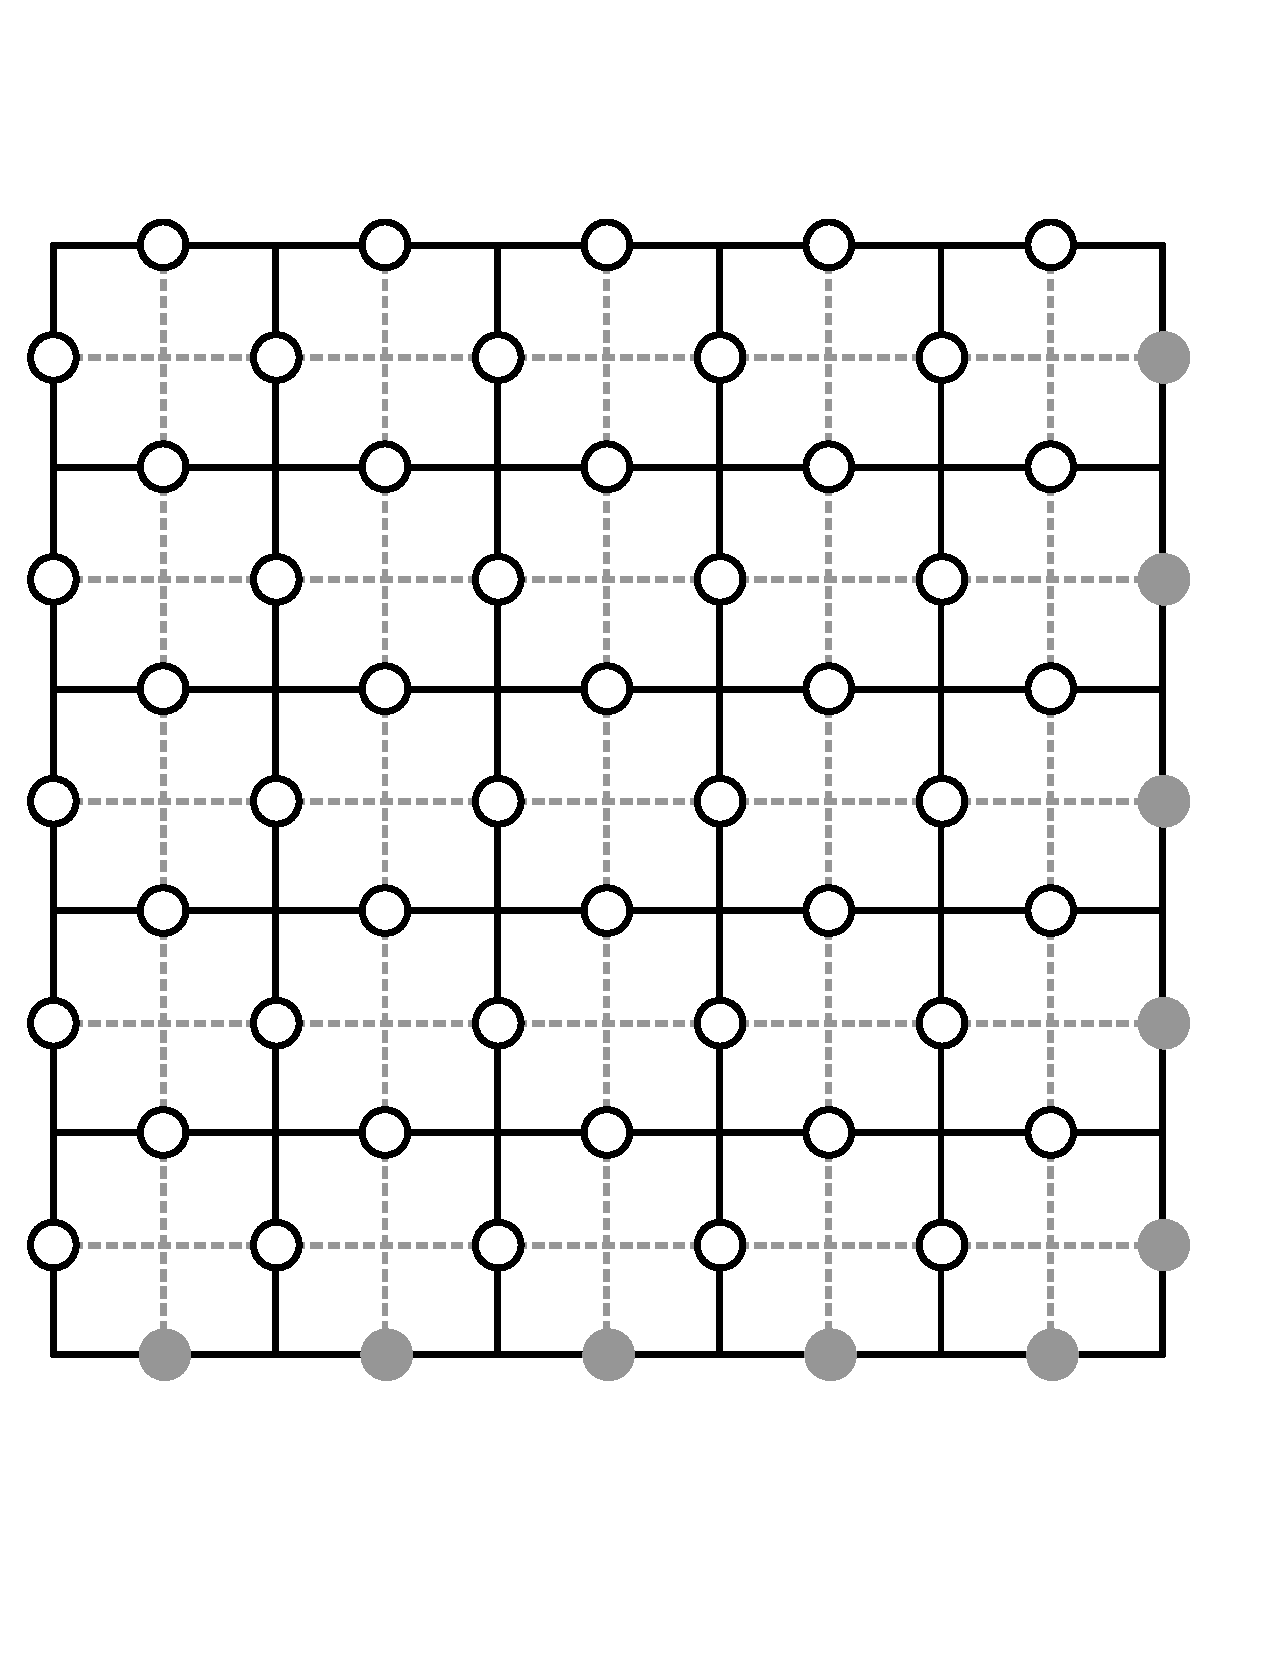
\includegraphics[width=\textwidth]{lattice.pdf}
             \caption{$(\nu_c,\nu_r) = (0,0)$}
             \label{fig:y trivial ground state}
         \end{subfigure}
         \hfill
         \begin{subfigure}[b]{0.2\textwidth}
             \centering
             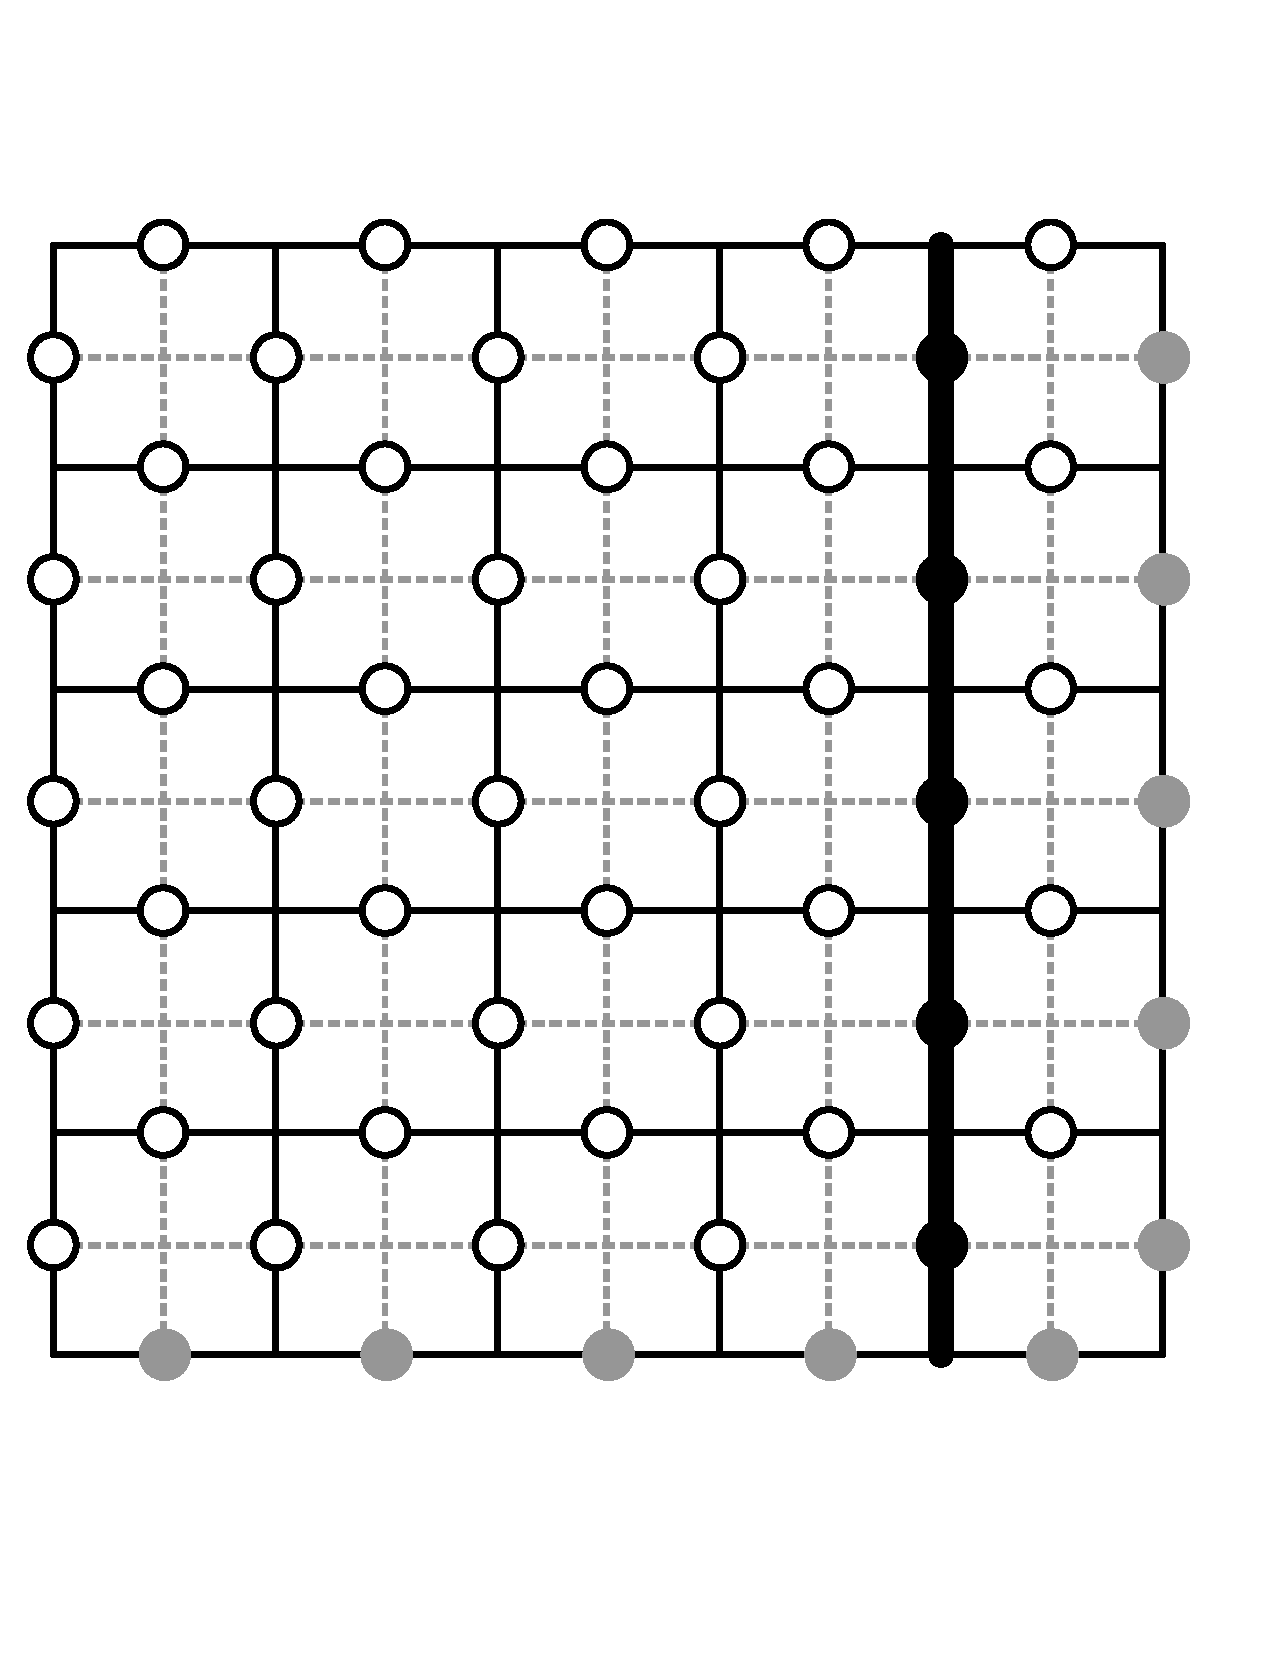
\includegraphics[width=\textwidth]{gs_v.pdf}
             \caption{$(\nu_c,\nu_r) = (1,0)$}
             \label{fig:vertical ground state}
         \end{subfigure}
         \hfill
         \begin{subfigure}[b]{0.2\textwidth}
             \centering
             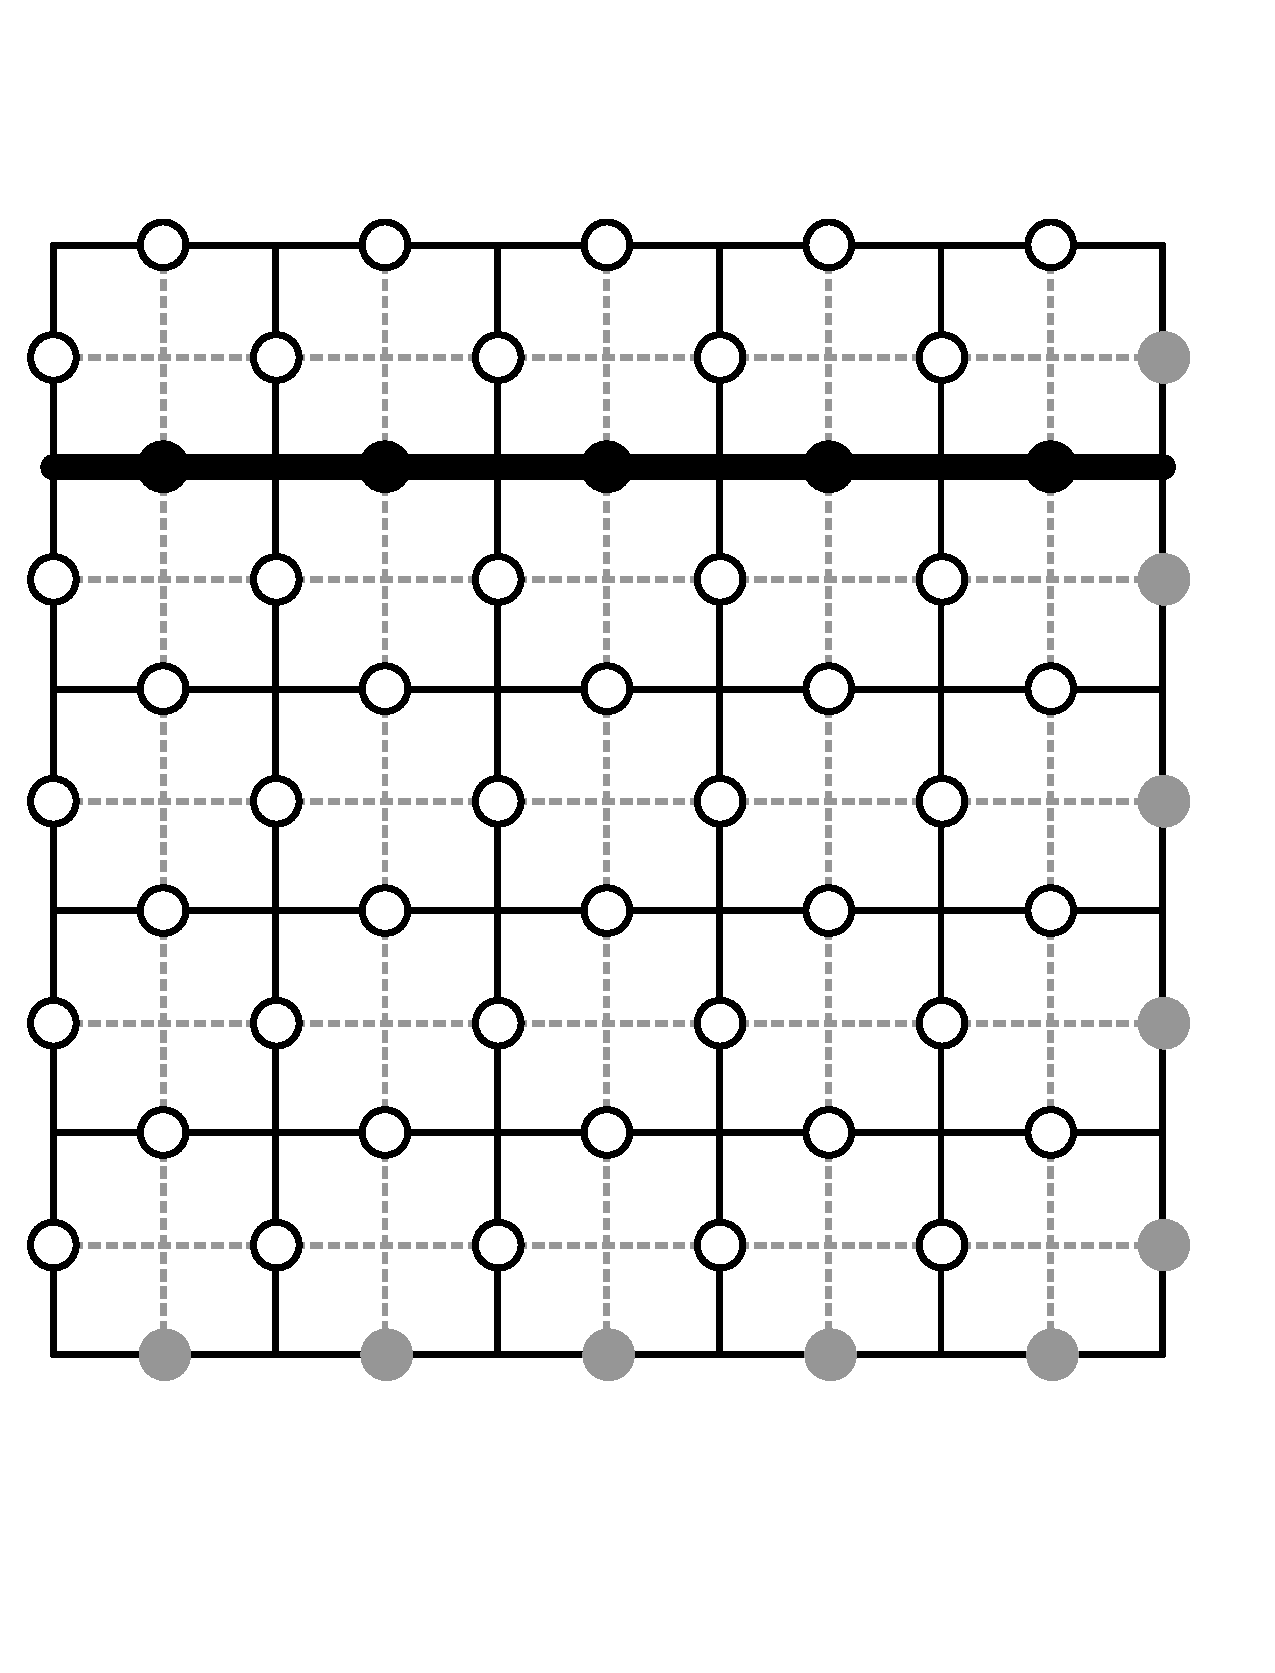
\includegraphics[width=\textwidth]{gs_h.pdf}
             \caption{$(\nu_c,\nu_r) = (0,1)$}
             \label{fig:horizontal ground state}
         \end{subfigure}
         \hfill
         \begin{subfigure}[b]{0.2\textwidth}
             \centering
             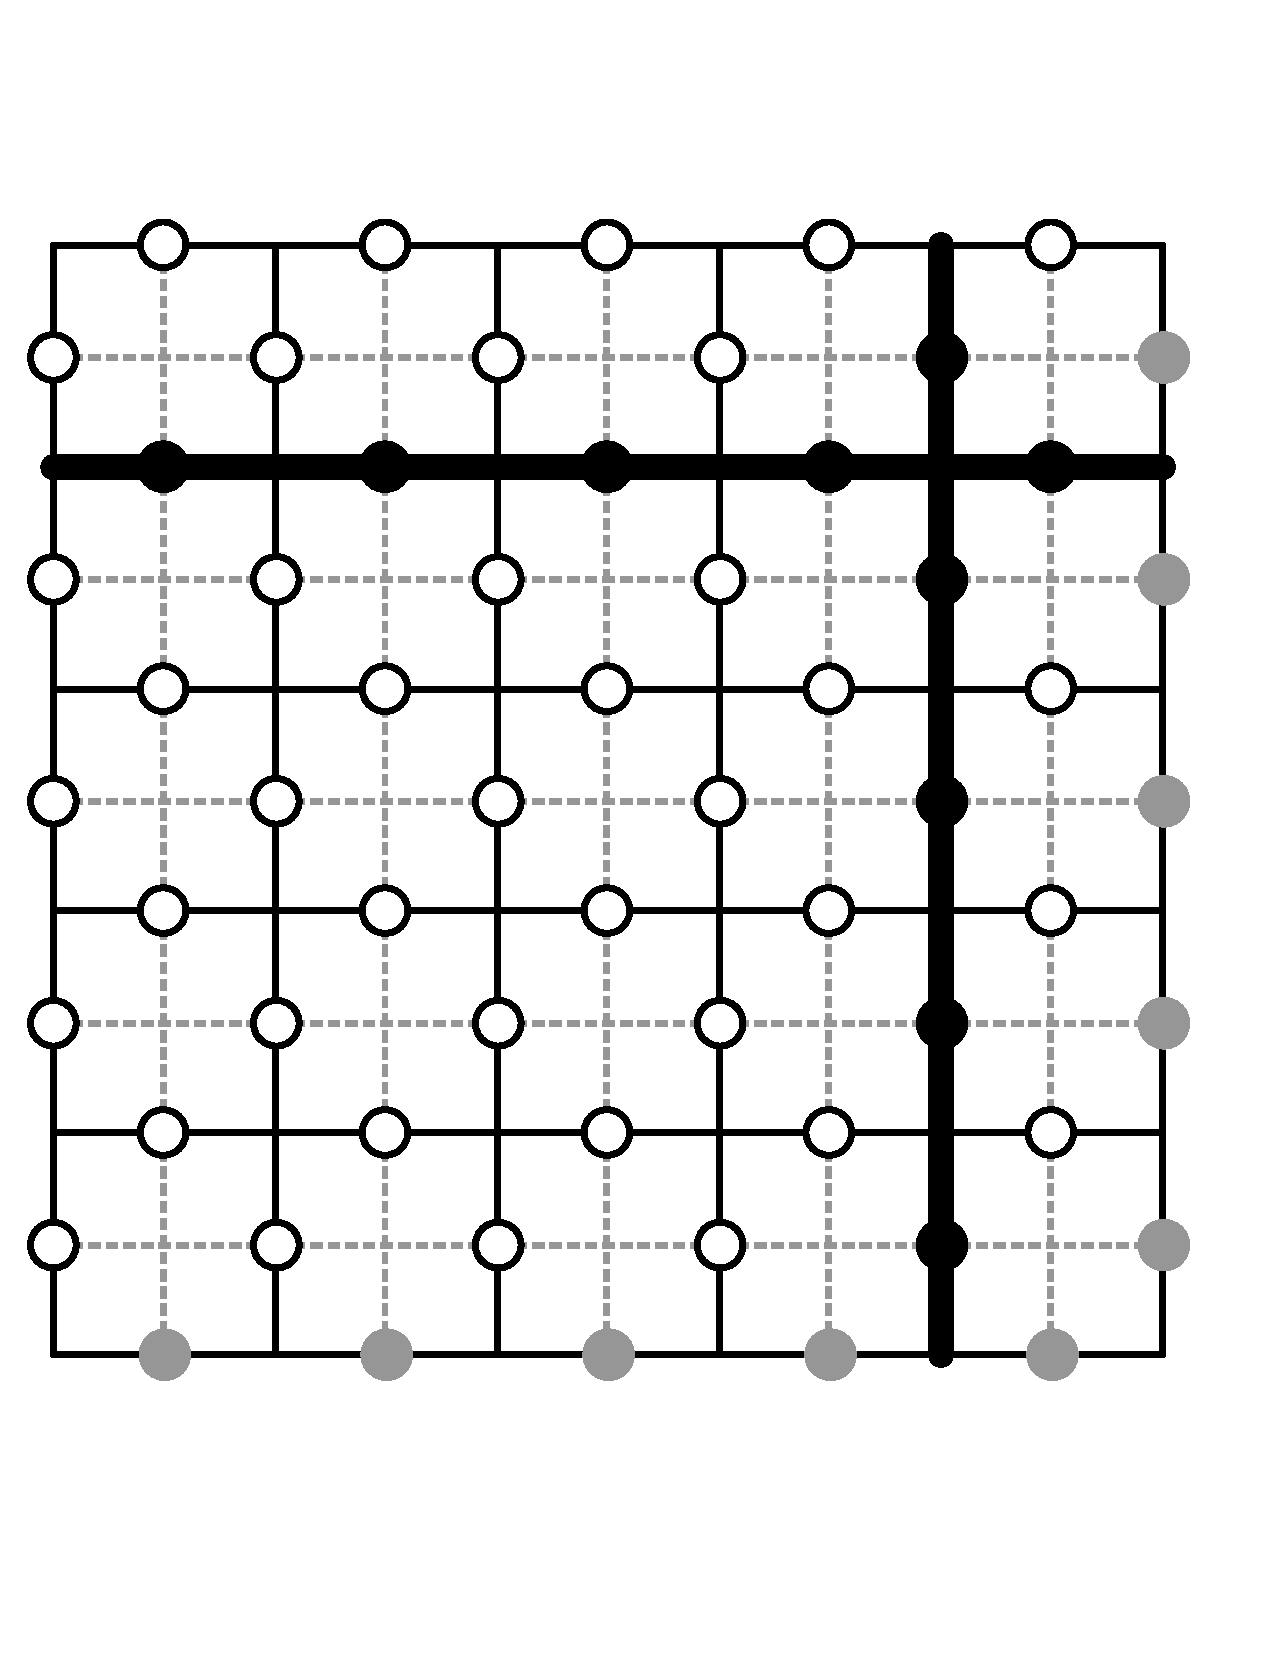
\includegraphics[width=\textwidth]{gs_m.pdf}
             \caption{$(\nu_c,\nu_r) = (1,1)$}
             \label{fig:mixed ground state}
         \end{subfigure}
            \caption{The four classes of non-contractible loops. Again, black edges represent $|1\rangle$ states.}
            \label{fig:three graphs}
    \end{figure}
\newpage
\subsection{Logical Operators}
In the toric code, logical operators are essential for encoding and manipulating quantum information. These are defined as acting non-trivially on ground state configurations without disturbing the stabilizer constraints of the system \cite{anintro}\cite{dennis2001}. Furthermore, logical operators commute with the system's Hamiltonian, $H_{TC}$. To better understand these operators, we will examine their form and behavior in relation to the lattice's non-contractible $1$-cycles and cocycles.\newline

To ensure that logical operators preserve the protected subspace $\mathcal{H_L}$, they must commute with both types of stabilizer operators, $A_v$ and $B_p$, for all $v\in V$ and $p\in P$. This can be shown formally if we consider some logical operator $L$ acting on a ground state $|\psi\rangle$, and impose that $L|\psi\rangle\in\mathcal{H_L}$:
    \begin{align}
        A_vL|\psi\rangle &= L|\psi\rangle\\
        &= LA_v|\psi\rangle\\
        (A_vL-LA_v)|\psi\rangle &= 0.
    \end{align}
It follows that $[A_v,L] = 0$. The exact same argument can be made for $B_p$, therefore it follows that if $L|\psi\rangle\in\mathcal{H_L}$, then $[L,H_{TC}] = 0$. We note that $(40)$ follows from the fact that $|\psi\rangle$ is a ground state, and therefore a $+1$ eigenstate of all stabilizers.
    \begin{definition}(Centralizer of a group).
        \emph{Let $G$ be a group, and $H\subset G$ be a subgroup. The centralizer of $H$ in $G$, is defined:}
            \begin{align}
                C_G(H) := \{g\in G|[g,h] = 0\enspace\forall\enspace h\in H\}.
            \end{align}
    \end{definition}
One can easily see that logical operators are elements of $C_{\textbf{Pauli}(N)}(\mathcal{S})/\mathcal{S}$, where $\textbf{Pauli}(N)$ is the Pauli group on $N$ qubits.\newline

In order for logical operators to act on ground states, they must involve comparable configurations to these states. More specifically, for logical operators to act on non-contractible $1$-cycles, they must themselves take the form of non-contractible $1$-cycles or cocycles Pauli $\sigma^z$ and $\sigma^x$ operators. This structure allows logical operators to transform ground states globally without local deformation, which is key to their role in protecting information.\newline

Having established that logical operators will take the form of non-contractible $1$-chains and cochains of $\sigma^x$ and $\sigma^z$ operators, it follows that we must study the commutation relations of such objects on the lattice and dual lattice. We define $1$-chains and cochains of Pauli $\sigma^x$ and $\sigma^z$ operators:
    \begin{align}
        Z_{c}:=\prod_{e_i\in c}\sigma^z_{e_i},\enspace\enspace\enspace Z_{c^*}:=\prod_{e^*_i\in c^*}\sigma^z_{e^*_i}\\
        X_c:=\prod_{e_i\in c}\sigma^x_{e_i},\enspace\enspace\enspace X_{c^*}:=\prod_{e^*_i\in c^*}\sigma^x_{e^*_i},
    \end{align}
where $c\in C_1$ and $c^*\in C_1^*$. Here $Z_{c}$ applies Pauli $\sigma^z$ operators along the edges of the $1$-chain(cochain) $c$($c^*$), and $X_{c}$($X_{c^*}$) applies Pauli $\sigma^x$ operators along the edges of the $1$-chain(cochain) $c$($c^*$). Conversely, $Z_{c^*}$ and $X_{c^*}$ apply $\sigma^x$ and $\sigma^x$ operators along the edges of the $1$-cochain $c^*$, respectively.\newline

The property $\{\sigma^x,\sigma^z\} = 0$, implies that an object in $(43)$ can only commute with an object in $(44)$ if their respective chains intersect an even number of times, in order to cancel out the anti-commutativity of their respective spin operators. To capture this behavior formally, we define the object $\langle c,c^*\rangle$ to represent the \emph{intersection number} between $c\in C_1$ and $c^*\in C^*_1$. It follows:
    \begin{align}
        [Z_{c^*},X_{c}] = [Z_{c},X_{c^*}] = (-1)^{\langle c,c^*\rangle}.
    \end{align}
This provides us with the necessary information to construct $Z$-type logical operators $\overline{Z}_{1,2}$ and $X$-type logical operators $\overline{X}_{1,2}$.\newline

For $\overline{Z}_{1,2}$ to commute with all stabilizer operators, they must overlap an even number of times with $A_v$ for all $v\in V$ (commutation with all $B_p$ follows trivially). The only way to achieve this is for $\overline{Z}_{1,2}$ to be $1$-chains on the lattice. The same reasoning can be applied to the construction of $\overline{X}_{1,2}$, as the only way for these objects to overlap with all $B_p$ an even number of times is for them to be $1$-cochains on the dual lattice. Reconciling this reasoning with the previously established assertion that $\overline{Z}_{1,2}$ and $\overline{X}_{1,2}$ must be non-contractible cycles and cocycles, we may finally define the encoded logical operators:
    \begin{align}
        \overline{Z}_{1,2} &= \prod_{c\in H_1}Z_c\\
        \overline{X}_{1,2} &= \prod_{c^*\in H^*_1}X_{c^*}.
    \end{align}
Being intrinsically related to the first homology and cohomology groups, the connection between the logical operators and the topology of the surface is clear. We may describe the four logical operators explicitly:
    \begin{enumerate}
        \item $\overline{Z}_1$; a closed $1$-chain of $\sigma^z$ operators wrapping the torus vertically
        \item $\overline{Z}_2$; a closed $1$-chain of $\sigma^z$ operators wrapping the torus horizontally
        \item $\overline{X}_1$; a closed $1$-cochain of $\sigma^x$ operators wrapping the torus vertically
        \item $\overline{Z}_2$; a closed $1$-cochain of $\sigma^x$ operators wrapping the torus vertically
    \end{enumerate}
    \begin{figure}[h]
         \centering
         \begin{subfigure}[b]{0.4\textwidth}
             \centering
             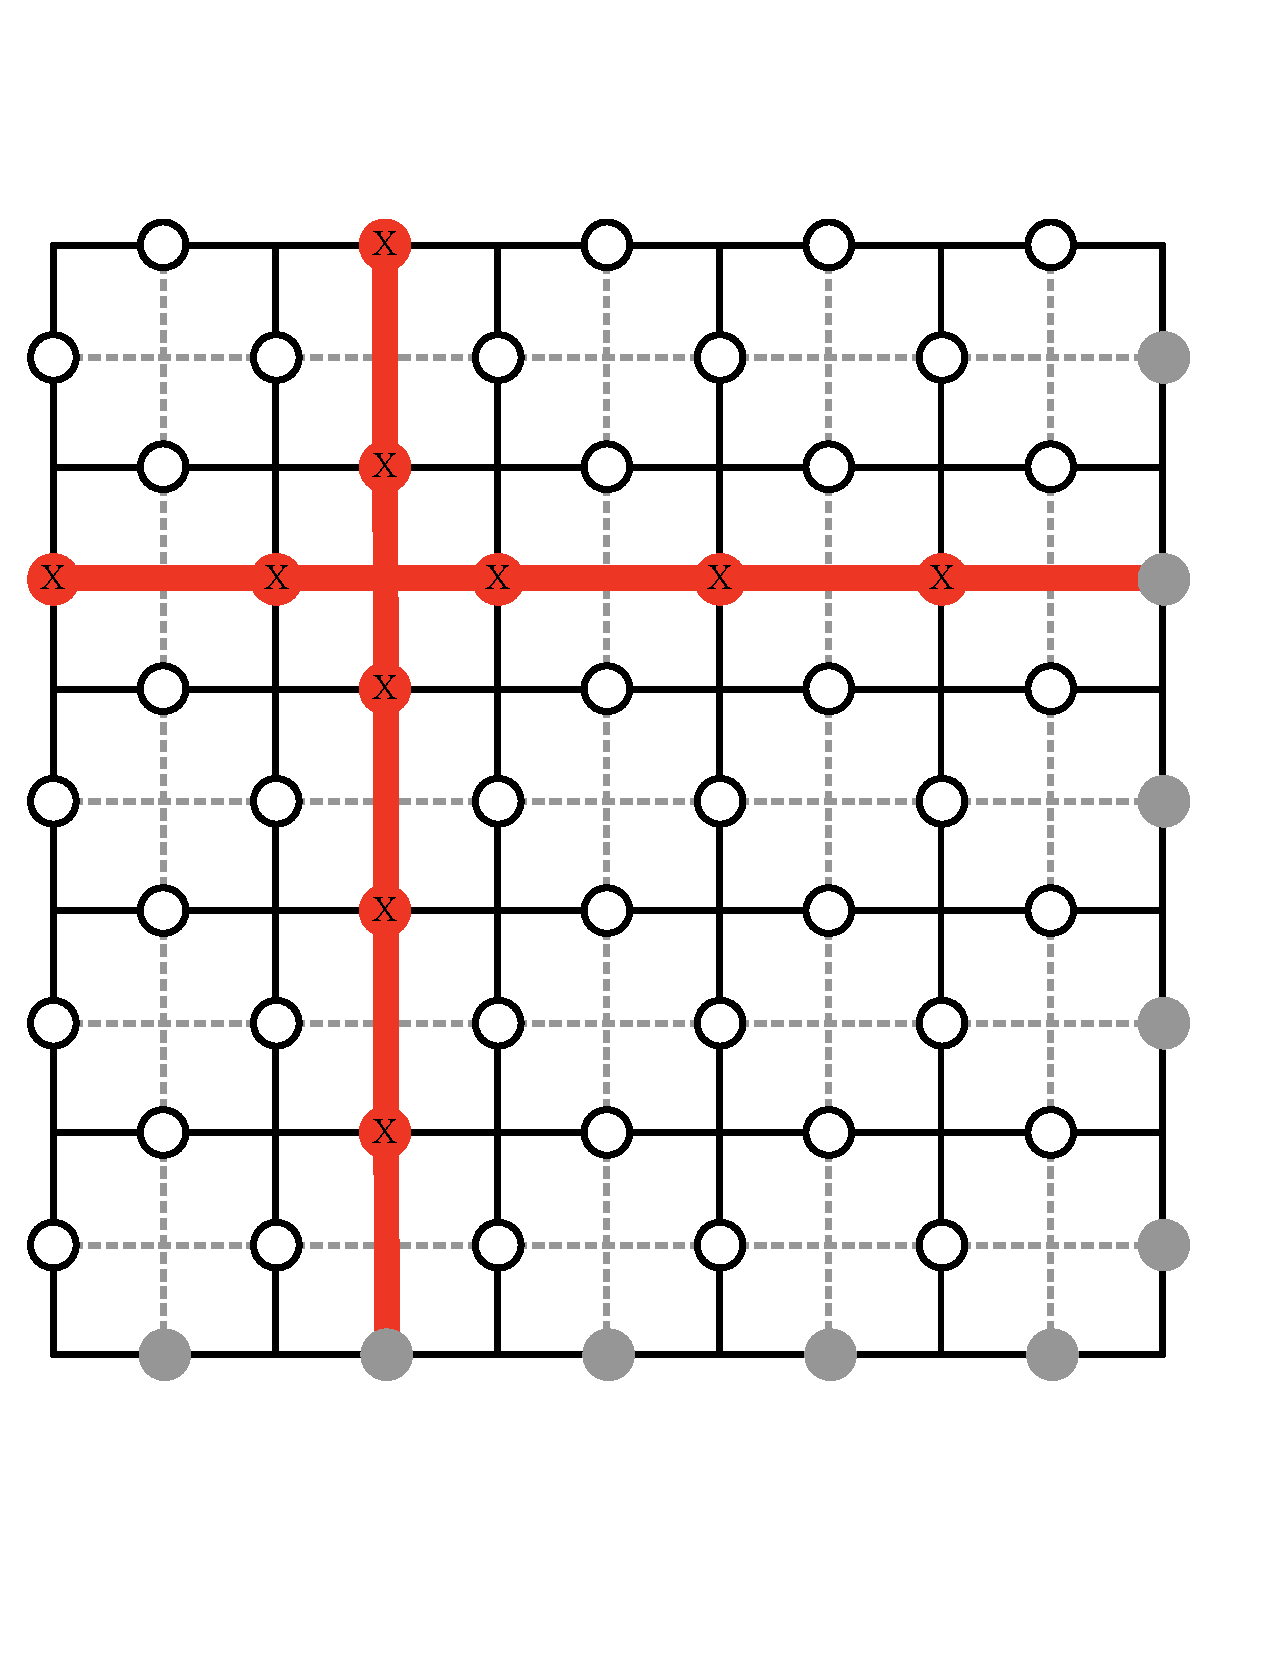
\includegraphics[width=\textwidth]{logx.pdf}
             \caption{$X$-type logical operators. $\overline{X}_1$ is horizontal, and $\overline{X}_2$ is vertical}
             \label{fig:logical x operators}
         \end{subfigure}
         \enspace\enspace\enspace
         \begin{subfigure}[b]{0.4\textwidth}
             \centering
             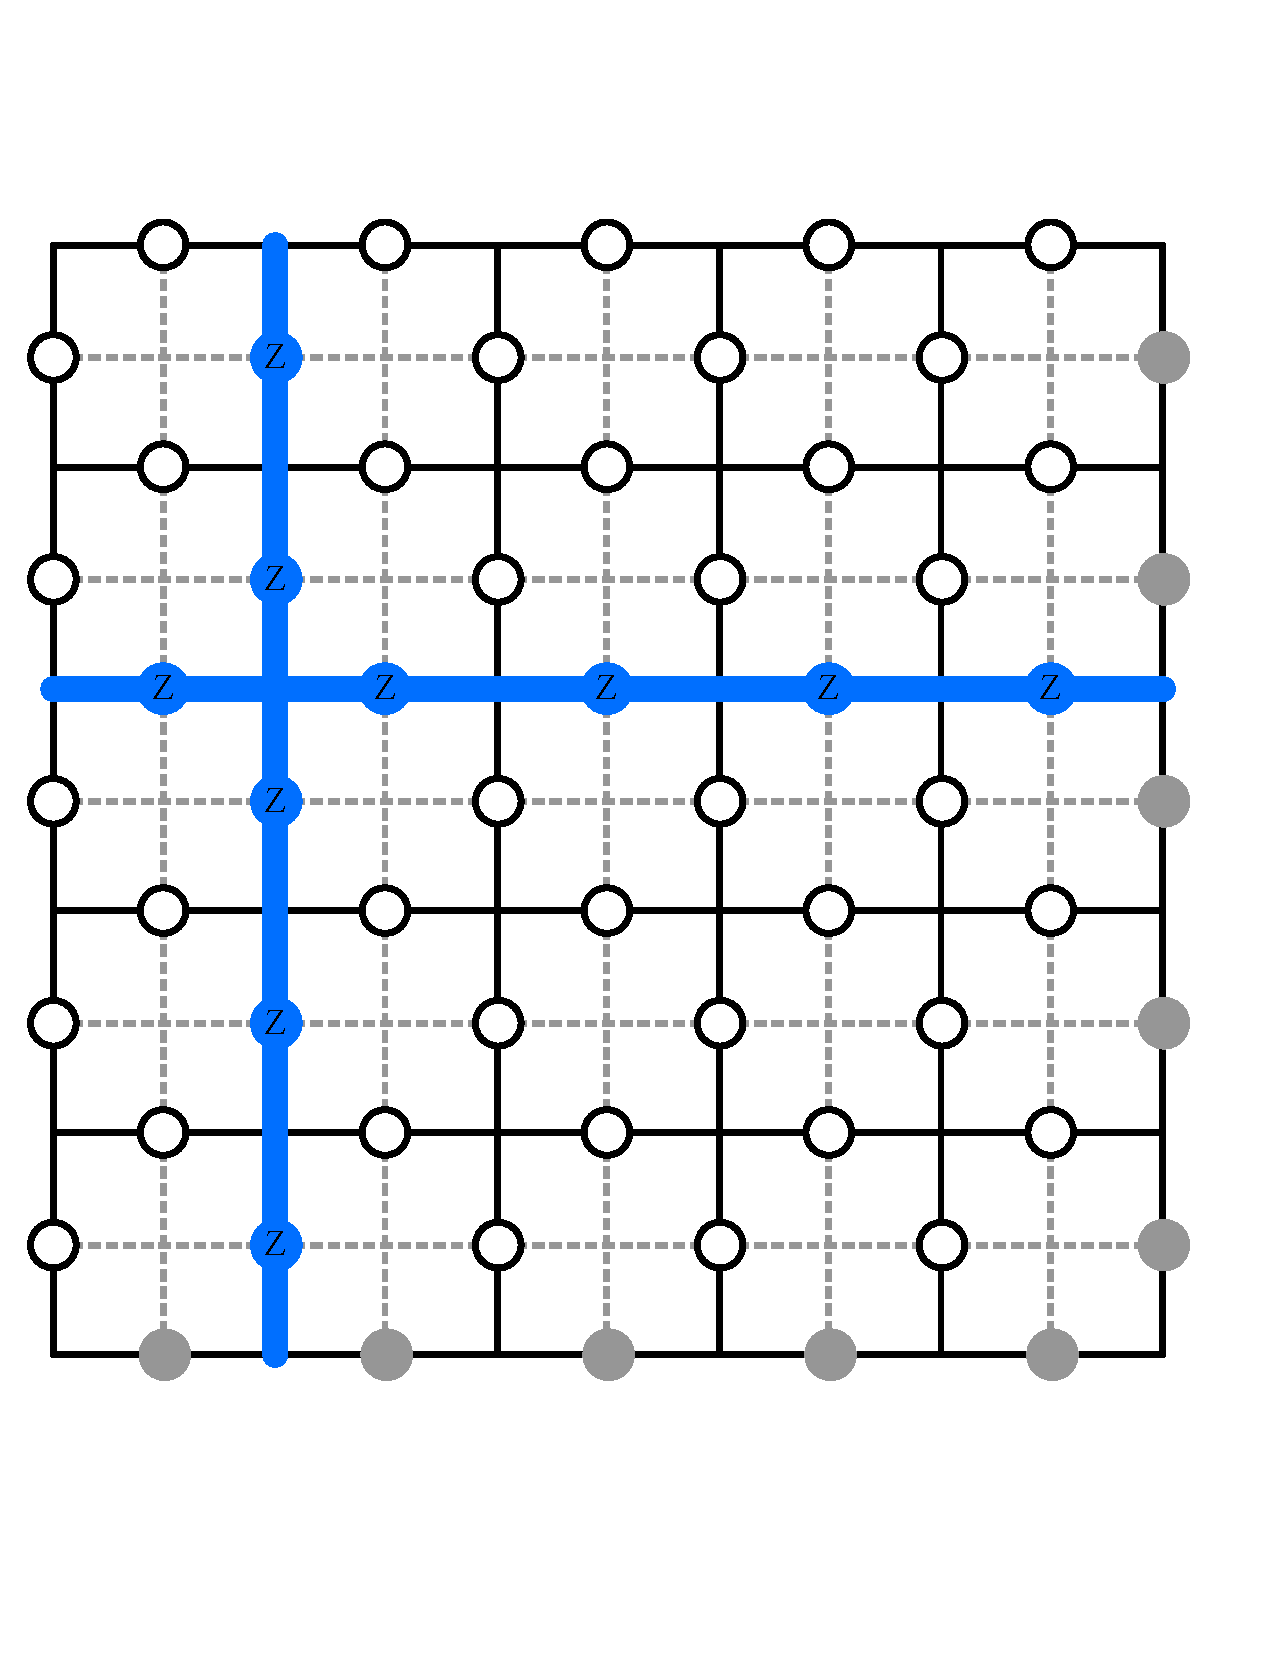
\includegraphics[width=\textwidth]{logz.pdf}
             \caption{$Z$-type logical operators. $\overline{Z}_1$ is vertical, and $\overline{Z}_2$ is horizontal}
             \label{fig:logical z operators}
         \end{subfigure}
            \caption{The four classes of logical operators}
            \label{fig:logical operators}
    \end{figure}
Each of these operators is unique up to homology. $Z$-type logical operators can be deformed by plaquette operators, into homologically equivalent closed $1$-chains. Consider $\overline{Z}_1$ acting along the $1$-chain $r_i := \{e_1,...,e_k\}\in H^v_1$, and apply a plaquette operator $B_{p_0}$ such that there exists $e_n\in r_i$ such that $e_n\in\partial_2p_0$. On the edge $e_n$, the superimposed $\sigma^z$ operators cancel out, deviating $\overline{Z}_1$'s path of operators around the boundary of $p_0$ while keeping the $1$-chain closed. Similarly, applying vertex operators to $X$-type logical operators can deform them into homologically equivalent closed $1$-cochains. Therefore, these logical operators are robust to local perturbations, as their non-contractible structure protects them from local error. The association of logical operators with homology classes underlines their topological protection, once again showing that the toric code is a promising candidate for fault-tolerant quantum computation.

\subsection{Excited States}
\subsubsection{String Operator Formalism}
Low energy excitations occur when the stabilizer constraints are violated, i.e. the configuration on $\mathcal{L}$ is no longer a simultaneous $+1$ eigenstate of all stabilizers. As such, these excitations represent local defects in the topologically ordered system. Excitations can be characterized by \emph{string operators}, which are products of Pauli operators along open $1$-chains and $1$-cochains on the lattice and dual lattice. There are two types of excitations: \emph{electric charges} $e$, corresponding to strings of $\sigma^z$ and \emph{magnetic vortices} $m$, corresponding to strings of $\sigma^x$. We will see that these excitations can be interpreted as quasiparticles of a $\ZZ_2$ gauge theory \cite{ellison2022}. The string operators are defined:
    \begin{align}
        S^z(t)=\prod_{e\in t}\sigma^z_e,\enspace\enspace\enspace S^x(t^*)=\prod_{e\in t^*}\sigma^x_e,\enspace\enspace\enspace t\in C_1,\enspace t^*\in C^*_1.
    \end{align}
If the endpoints of an $e$-type excitation and $m$-type excitation coincide on a plaquette - formally, for $S^z(t)$ with $t := \{e_1,...,e_n\}$ and $S^x(t^*)$ with $t^* := \{e^*_1,...,e^*_k\}$, if there exists some $p_0\in P$ such that $\{e_j^*\}_{j\in \{1,k\}}\in\partial_2p_0$ and $\partial_1\{e_i\}_{i\in \{1,n\}}\cap\partial\{e\}_{e\in\partial_2p_0}\neq\emptyset$ - we say that we have a \emph{dyon}, or $\epsilon$-type excitations.
    \begin{figure}[h]
         \centering
         \begin{subfigure}[b]{0.4\textwidth}
             \centering
             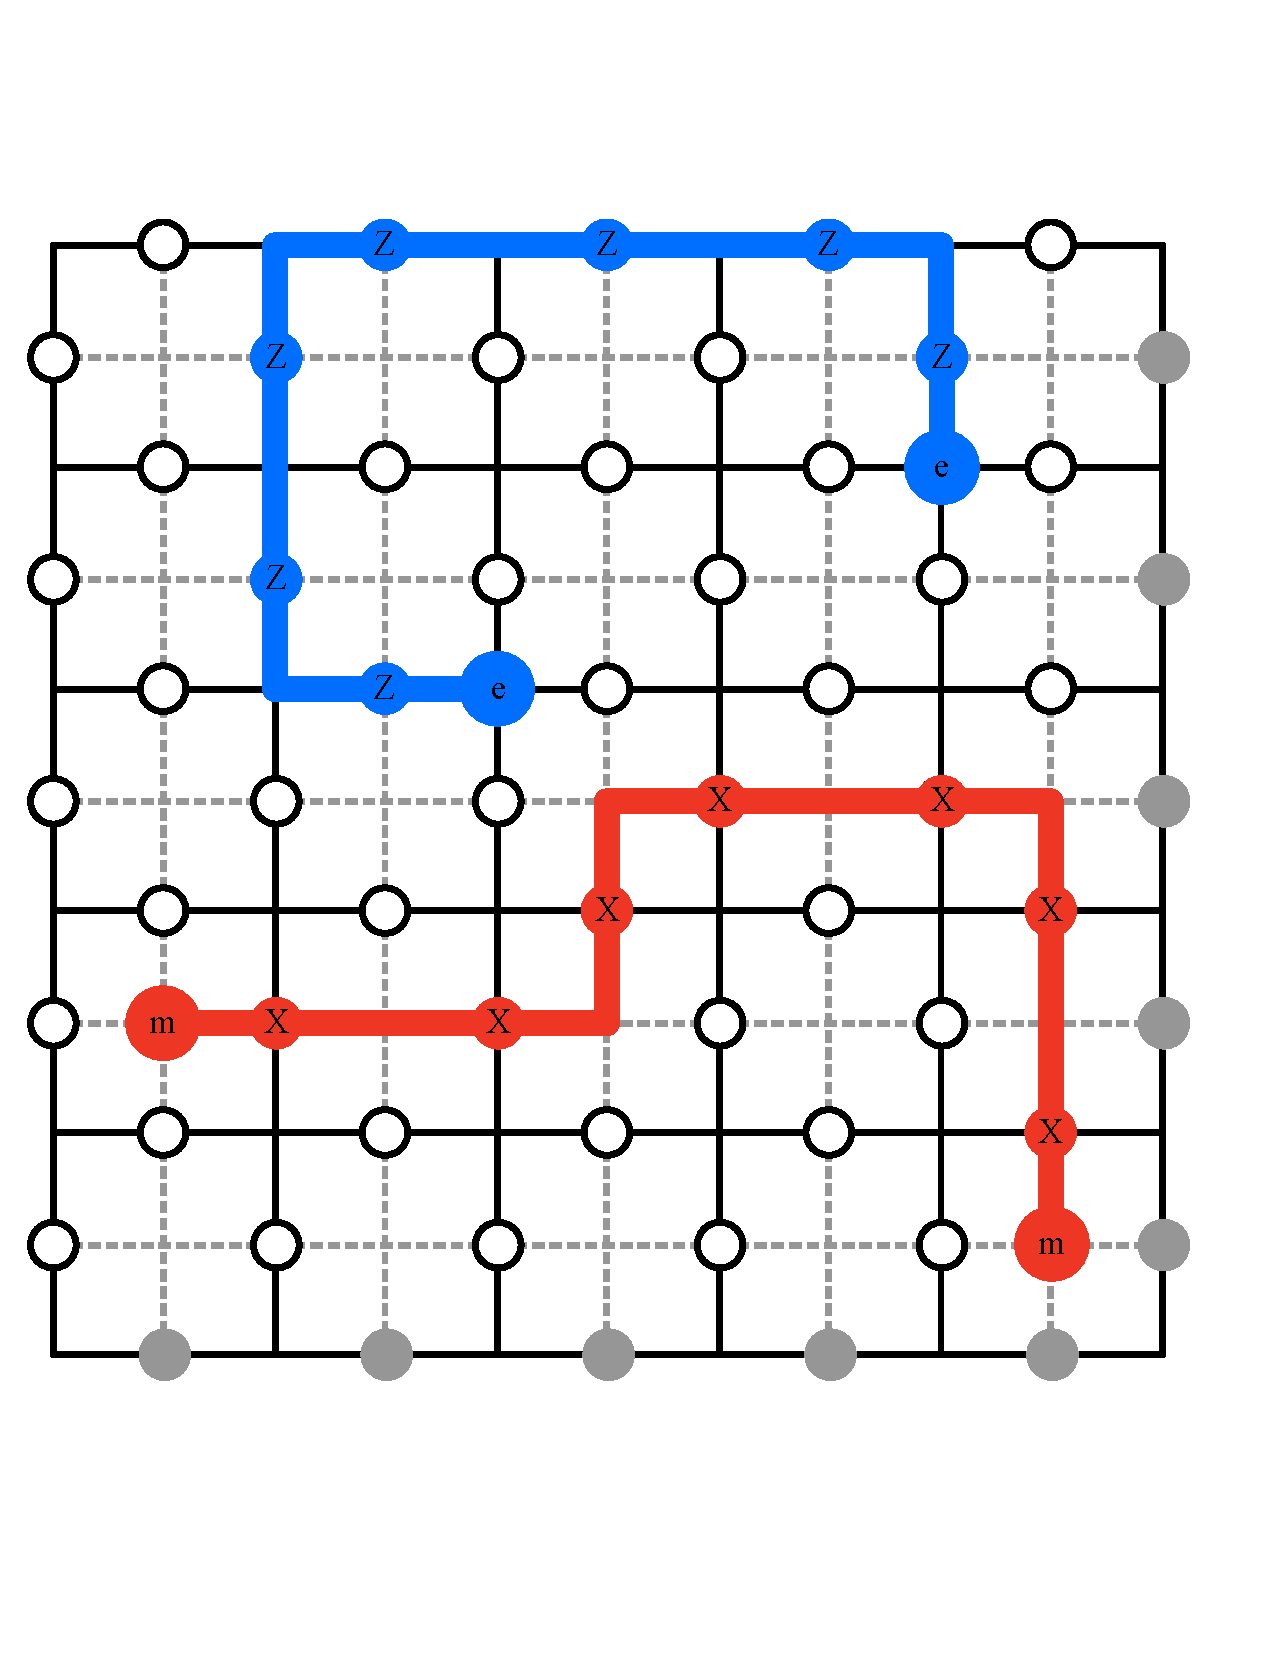
\includegraphics[width=\textwidth]{strings.pdf}
             \caption{Strings of $\sigma^z$ operators (blue) on the lattice result in electric excitations at their endpoints, and strings of $\sigma^x$ operators (red) on the dual lattice result in magnetic vortices at their endpoints.}
             \label{fig:e and m excitations}
         \end{subfigure}
         \enspace\enspace\enspace
         \begin{subfigure}[b]{0.4\textwidth}
             \centering
             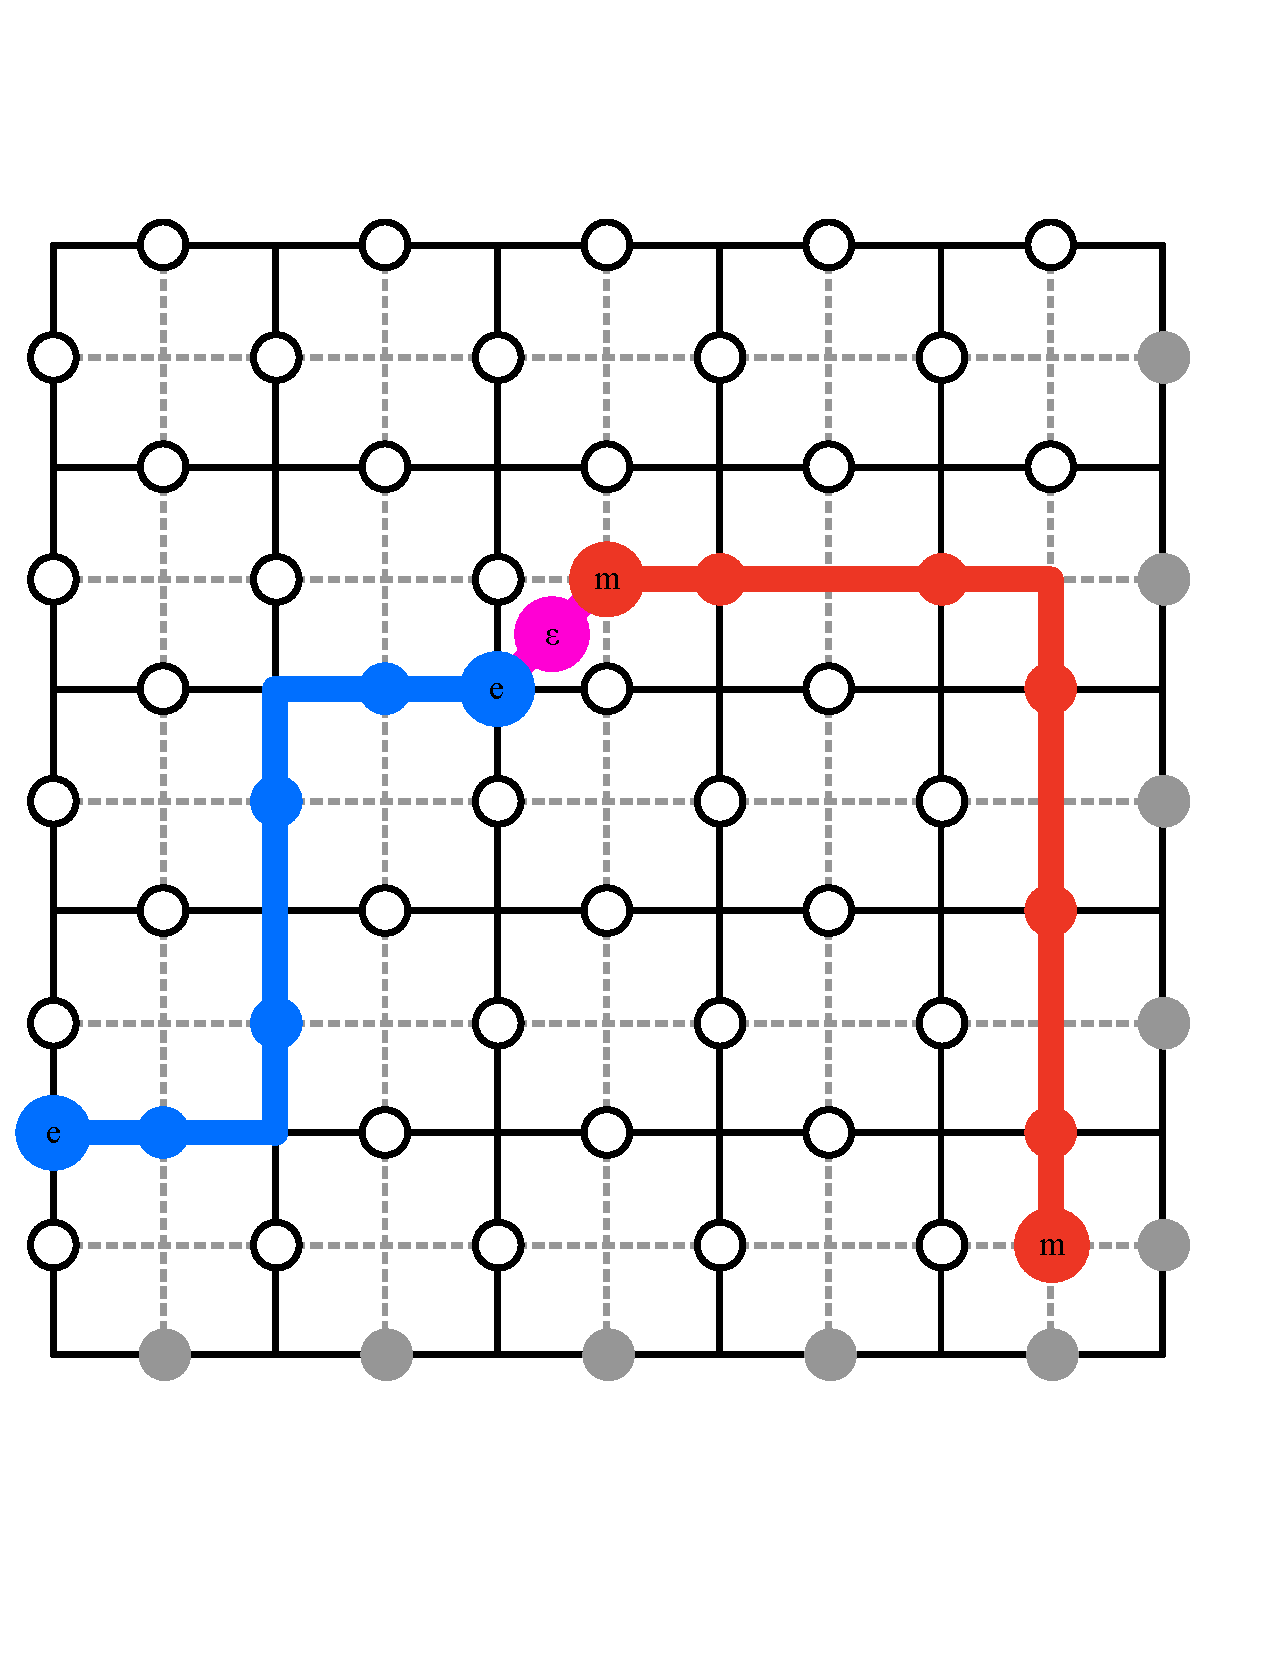
\includegraphics[width=\textwidth]{dyon.pdf}
             \caption{When magnetic and electric excitations coincide on a plaquette, a dyon is produced (pink).\newline\newline}
             \label{fig:dyon}
         \end{subfigure}
            \caption{The three types of excitations on the lattice.}
            \label{fig:excitations}
    \end{figure}

String operators violate the stabilizer constraints at their endpoints, resulting in topological defects commonly referred to as \emph{quasiparticles}. To see this, let $|\psi\rangle$ be a ground state, and consider an $e$-type excited state $|\phi^z(t)\rangle = S^z(t)|\psi\rangle$ with $t := \{e_1,...,e_n\}$ that terminates on vertices $v_1,v_n\in V$. Without loss of generality, we assign $v_1\in\partial_1e_1$ and $v_n\in\partial_1e_n$. We focus on the endpoint $v_1$, labeling the remaining edges incident on $v_1$ with $e_A,e_B,e_C$, and apply a vertex operator at $v_1$:
    \begin{align}
        A_{v_1}|\phi^z(t)\rangle &= A_{v_1}S^z(t)|\psi\rangle\\
        &= \prod_{e\mid v_1\in\partial_1e}\sigma^x_e\prod_{e\in t}\sigma^z_e|\psi\rangle\\
        &= \sigma^x_{e_A}\sigma^x_{e_B}\sigma^x_{e_C}\sigma^x_{e_1}\sigma^z_{e_1}\sigma^z_{e_2}...\sigma^z_{e_n}|\psi\rangle\\
        &= -\sigma^x_{e_A}\sigma^x_{e_B}\sigma^x_{e_C}\sigma^z_{e_1}\sigma^x_{e_1}\sigma^z_{e_2}...\sigma^z_{e_n}|\psi\rangle\\
        &= -\sigma^z_{e_1}\sigma^z_{e_2}...\sigma^z_{e_n}\sigma^x_{e_A}\sigma^x_{e_B}\sigma^x_{e_C}\sigma^x_{e_1}|\psi\rangle\\
        &= -S^z(t)A_{v_0}|\psi\rangle\\
        &= -S^z(t)|\psi\rangle\\
        &= -|\phi^z(t)\rangle.
    \end{align}
Where in $(52)$ follows from the property $\{\sigma^x,\sigma^z\} = 0$, and $(55)$ follows from the fact that $|\psi\rangle$ is a ground state. Thus $|\phi^z(t)\rangle$ is a $-1$ eigenstate of $A_{v_1}$, and therefore violates the stabilizer conditions at its endpoints. A similar argument can be made for $m$-type excitations. It follows that the energy cost for creating a pair of excitations is $+2$, because the eigenvalues of the stabilizer operators at the endpoints of the strings are flipped from $+1$ to $-1$, raising the system’s energy by $+2$.\newline

It is very important to note that $e$-type and $m$-type quasiparticles always occur in pairs. To see this, suppose that there exists an operator $C$ that creates a single excitation by acting on a ground state $|\psi\rangle$. As such, $C$ anti-commutes with \emph{only one} of the stabilizers on the lattice. Without loss of generality, we assume $C$ anti-commutes with $A_{v_0}$ for $v_0\in V$, and commutes with all other $A_v$ and $B_p$ for $v\in V\setminus\{v_0\}$ and $p\in P$. If we apply the product of all vertex stabilizers $\prod_{v\in V} A_v$ to the state $C|\psi\rangle$, we have:
    \begin{align}
        (\prod_{v\in V}A_v)C|\psi\rangle &= (\prod_{v\in V\setminus\{v_0\}}A_v)A_{v_0}C|\psi\rangle\\
        &= -(\prod_{v\in V\setminus\{v_0\}}A_v)CA_{v_0}|\psi\rangle\\
        &= -C(\prod_{v\in V}A_v)|\psi\rangle\\
        &= -C|\psi\rangle.
    \end{align}
To obtain $(60)$, we applied property 2 from Section $2.2$. The very same property can be applied to the left-hand-side of $(57)$, resulting in:
    \begin{align}
        C|\psi\rangle = -C|\psi\rangle.
    \end{align}
This implies that $C|\psi\rangle = 0$, meaning that the operators $C$ annihilates the ground state, making it impossible to create an isolated excitation. Therefore, any valid excitation must create a pair of quasiparticles. This result can also be understood in the language of algebraic topology by noting that excitations correspond to violations of the conditions defined by the first homology group $H_1$. The string operators map elements from $H_1$ to new configurations that do not correspond to boundaries in $B_1$, which leads to the creation of defects in the topology.

\subsubsection{Transporting Quasiparticles}
One of the most important aspects of excitations on the lattice is their anyonic behavior, which is reflected in their exchange statistics. To study this behavior rigorously, some formalism must first be developed. A quasiparticle can be transported across the lattice through the strategic application of string operators, Figure~\ref{fig:moving}. More specifically, an $e$-type quasiparticle at $v_1\in V$ can be transported to another vertex $v_n\in V$ by applying the string operator $S^z(l)$ with $\partial_1l := \{v_1,v_n\}$. This action annihilates the original quasiparticle at $v_1$ and creates a new one at $v_n$. This behavior can be formalized by considering an excited state $|\phi^z(t)\rangle = S^z(t)|\psi\rangle$ with $\partial_1t := \{v_0,v_1\}$, and a $l\in C_1$ with $\partial_1l := \{v_1,v_n\}$:
    \begin{align}
        S^z(l)|\phi^z(t)\rangle &= S^z(l)S^z(t)|\psi\rangle\\
        &= \prod_{e\in l}\sigma^z_e\prod_{e\in t}\sigma^z_e|\psi\rangle\\
        &= \prod_{e\in\gamma}\sigma^z_e|\psi\rangle\\
        &= S^z(\gamma)|\psi\rangle\\
        &= |\phi^z(\gamma)\rangle,
    \end{align}
where $\gamma\in C_1$ with $\partial_1\gamma := \{v_0,v_n\}$, which follows from the addition mechanism of $1$-chains. We verify that the quasiparticle at $v_1$ is annihilated by noting that the new string operator $S^z(\gamma)$ is no longer open at $v_1$, and $|\{e\in E|v_1\in\partial_1e\}\cap\{e\in\gamma|v_1\in\partial_1e\}| = 2$. Therefore $A_{v_1}|\phi^z(\gamma)\rangle = |\phi^z(\gamma)\rangle$, and there is no quasiparticle at $v_1$.
    \begin{figure}[h]
         \centering
         \begin{subfigure}[b]{0.4\textwidth}
             \centering
             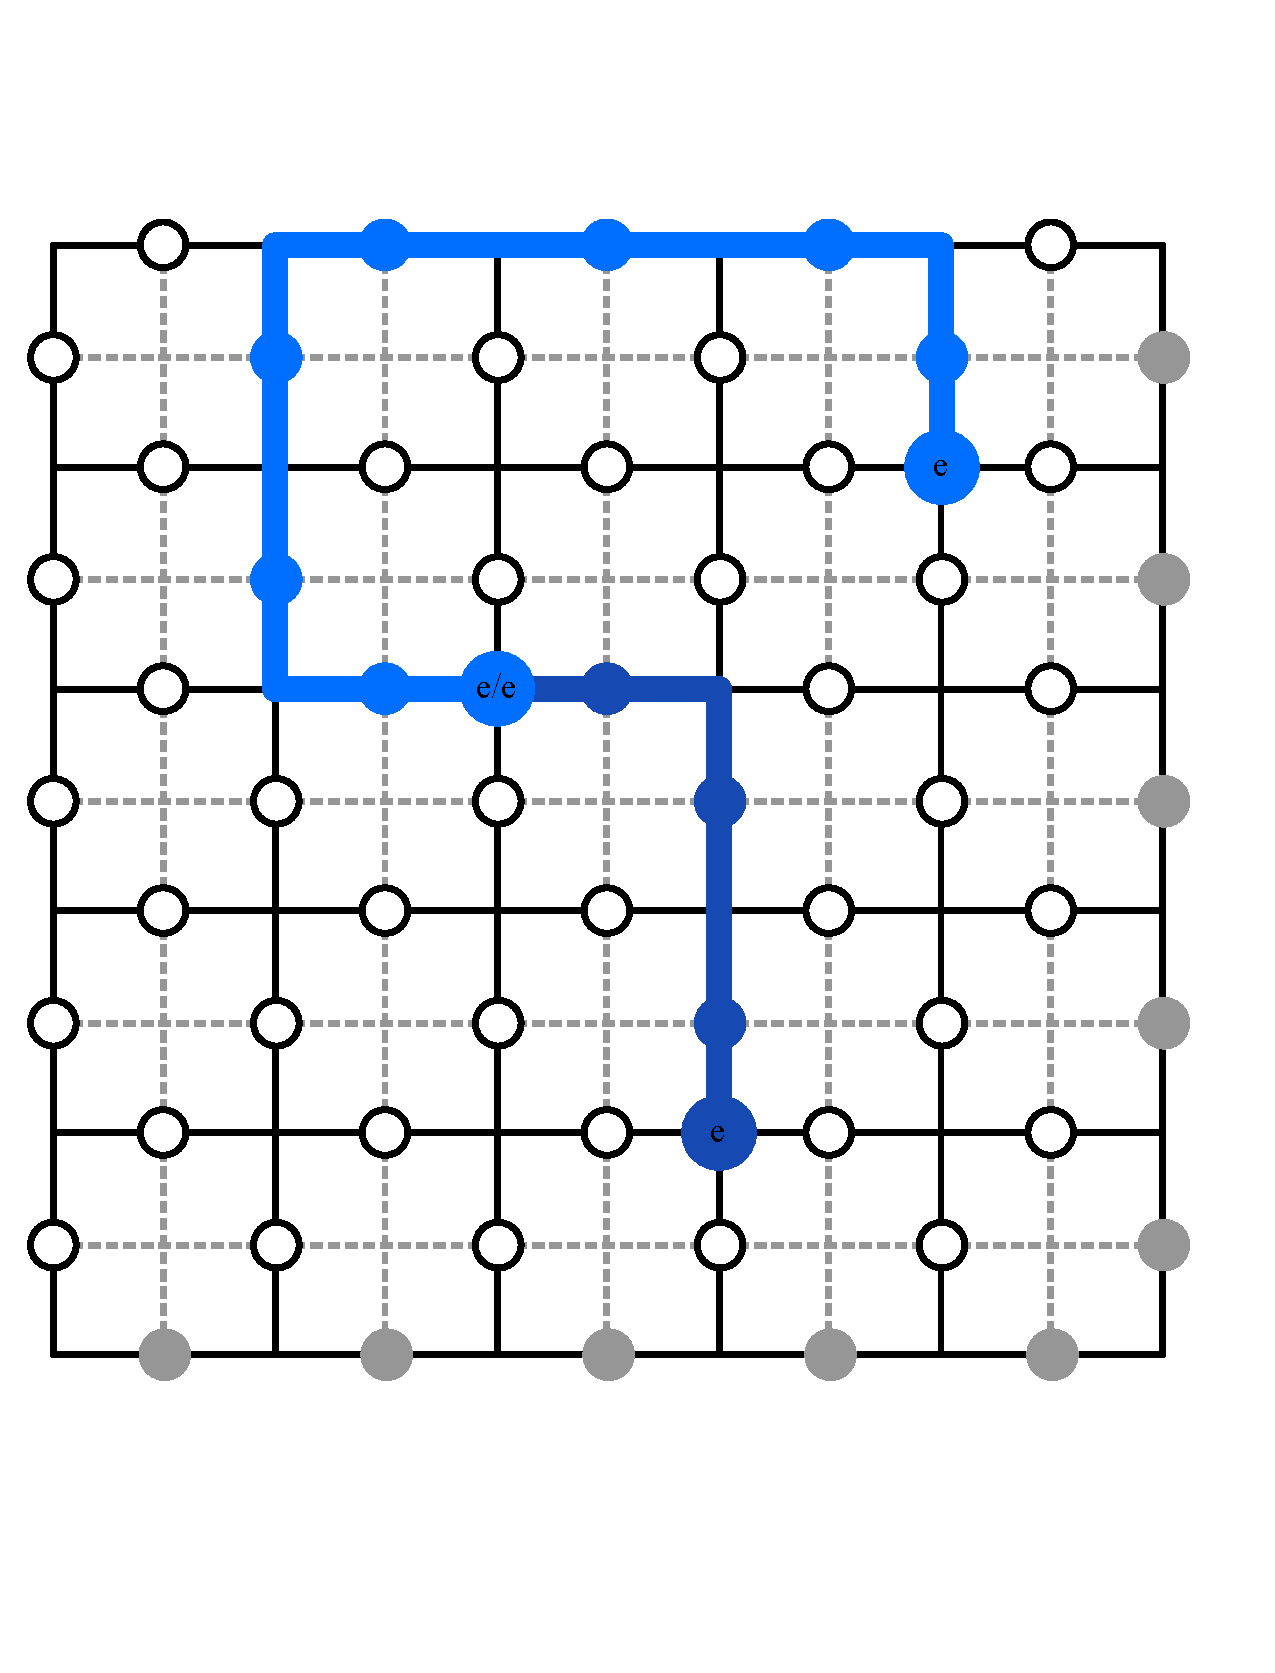
\includegraphics[width=\textwidth]{trans1.pdf}
             \label{fig:transport 1}
         \end{subfigure}
         \enspace\enspace\enspace
         \begin{subfigure}[b]{0.4\textwidth}
             \centering
             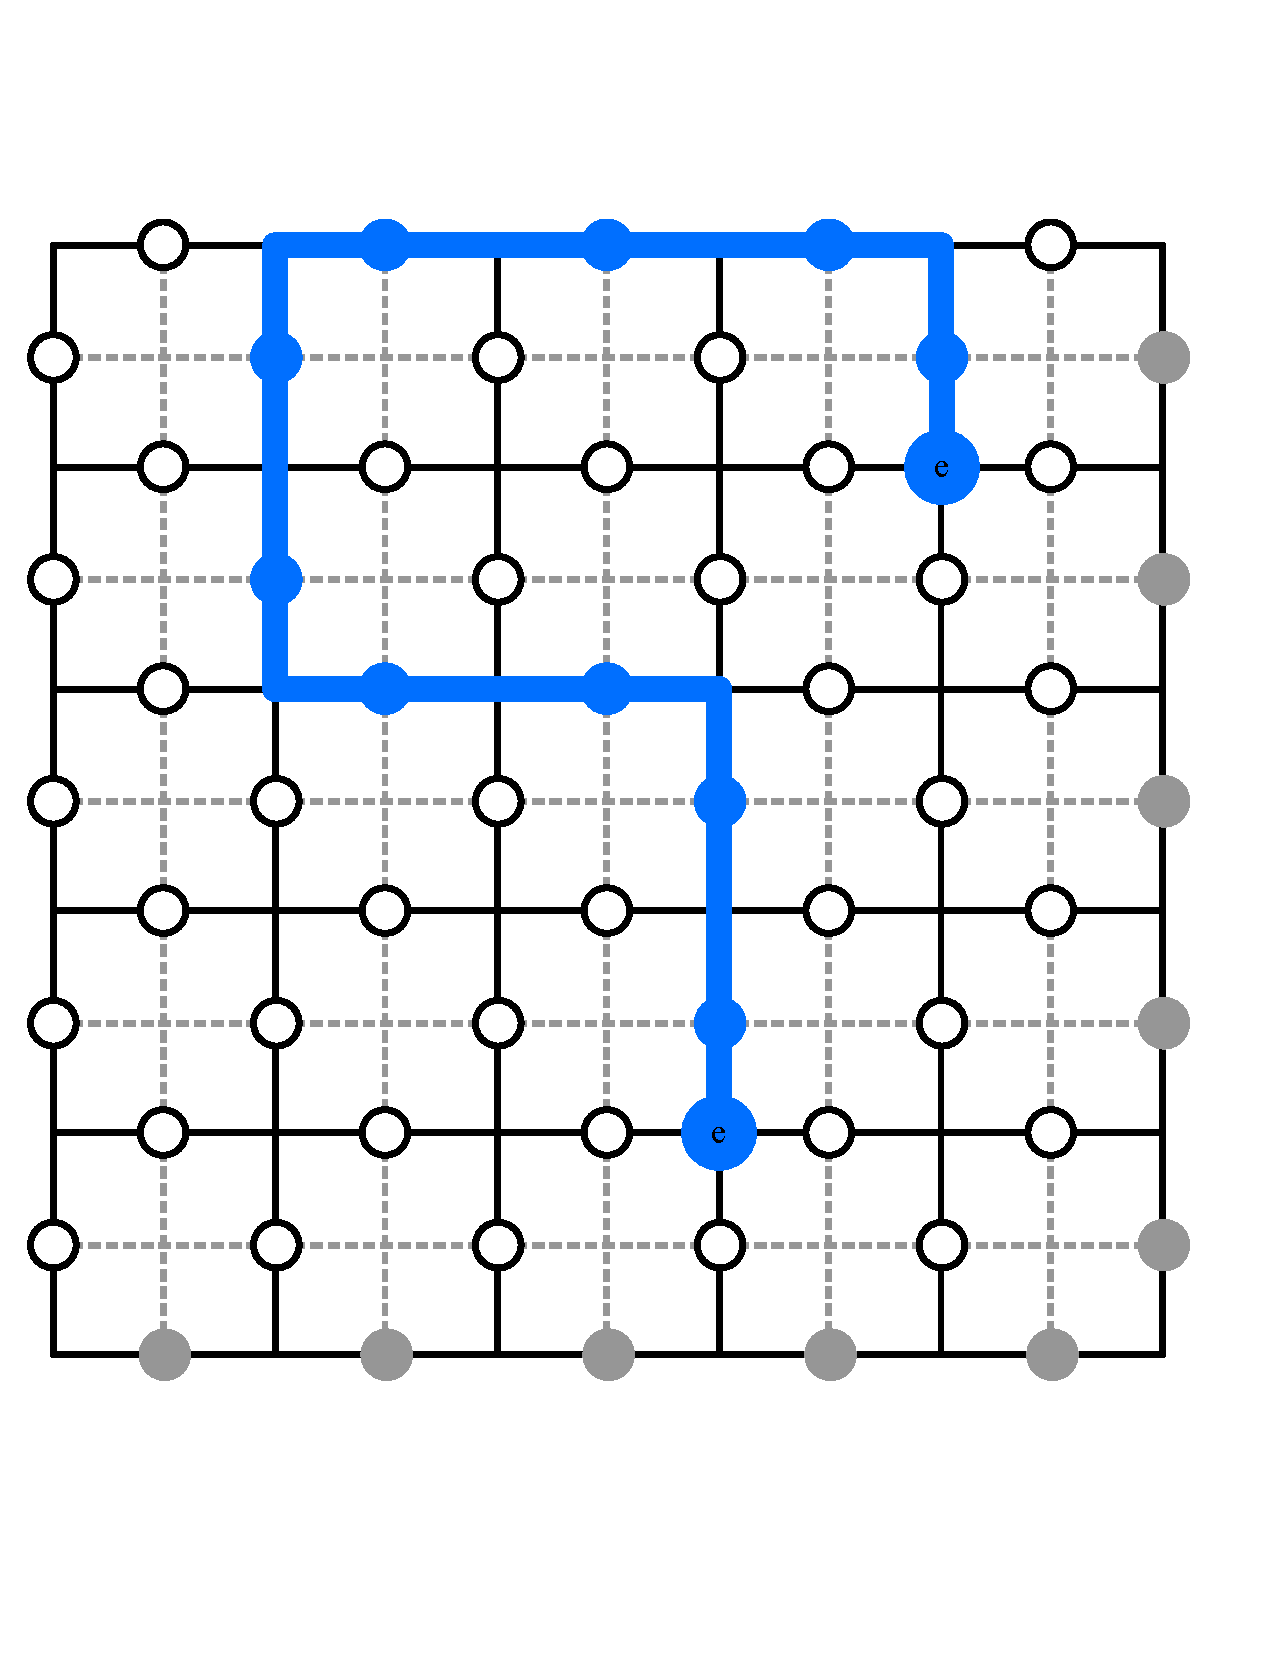
\includegraphics[width=\textwidth]{trans2.pdf}
             \label{fig:transport 2}
         \end{subfigure}
            \caption{When a $\sigma^z$-type string operator is applied to the endpoint of an existing excitation (left), the result is a new electric charge across the lattice (right).}
            \label{fig:moving}
    \end{figure}

Quasiparticle pairs can be annihilated by transporting one of the quasiparticles to the site of its pair. By combining string operators on $1$-chains with the same endpoints, a closed loop is formed, thereby returning the system to the ground state.
    \begin{figure}[h]
         \centering
         \begin{subfigure}[b]{0.4\textwidth}
             \centering
             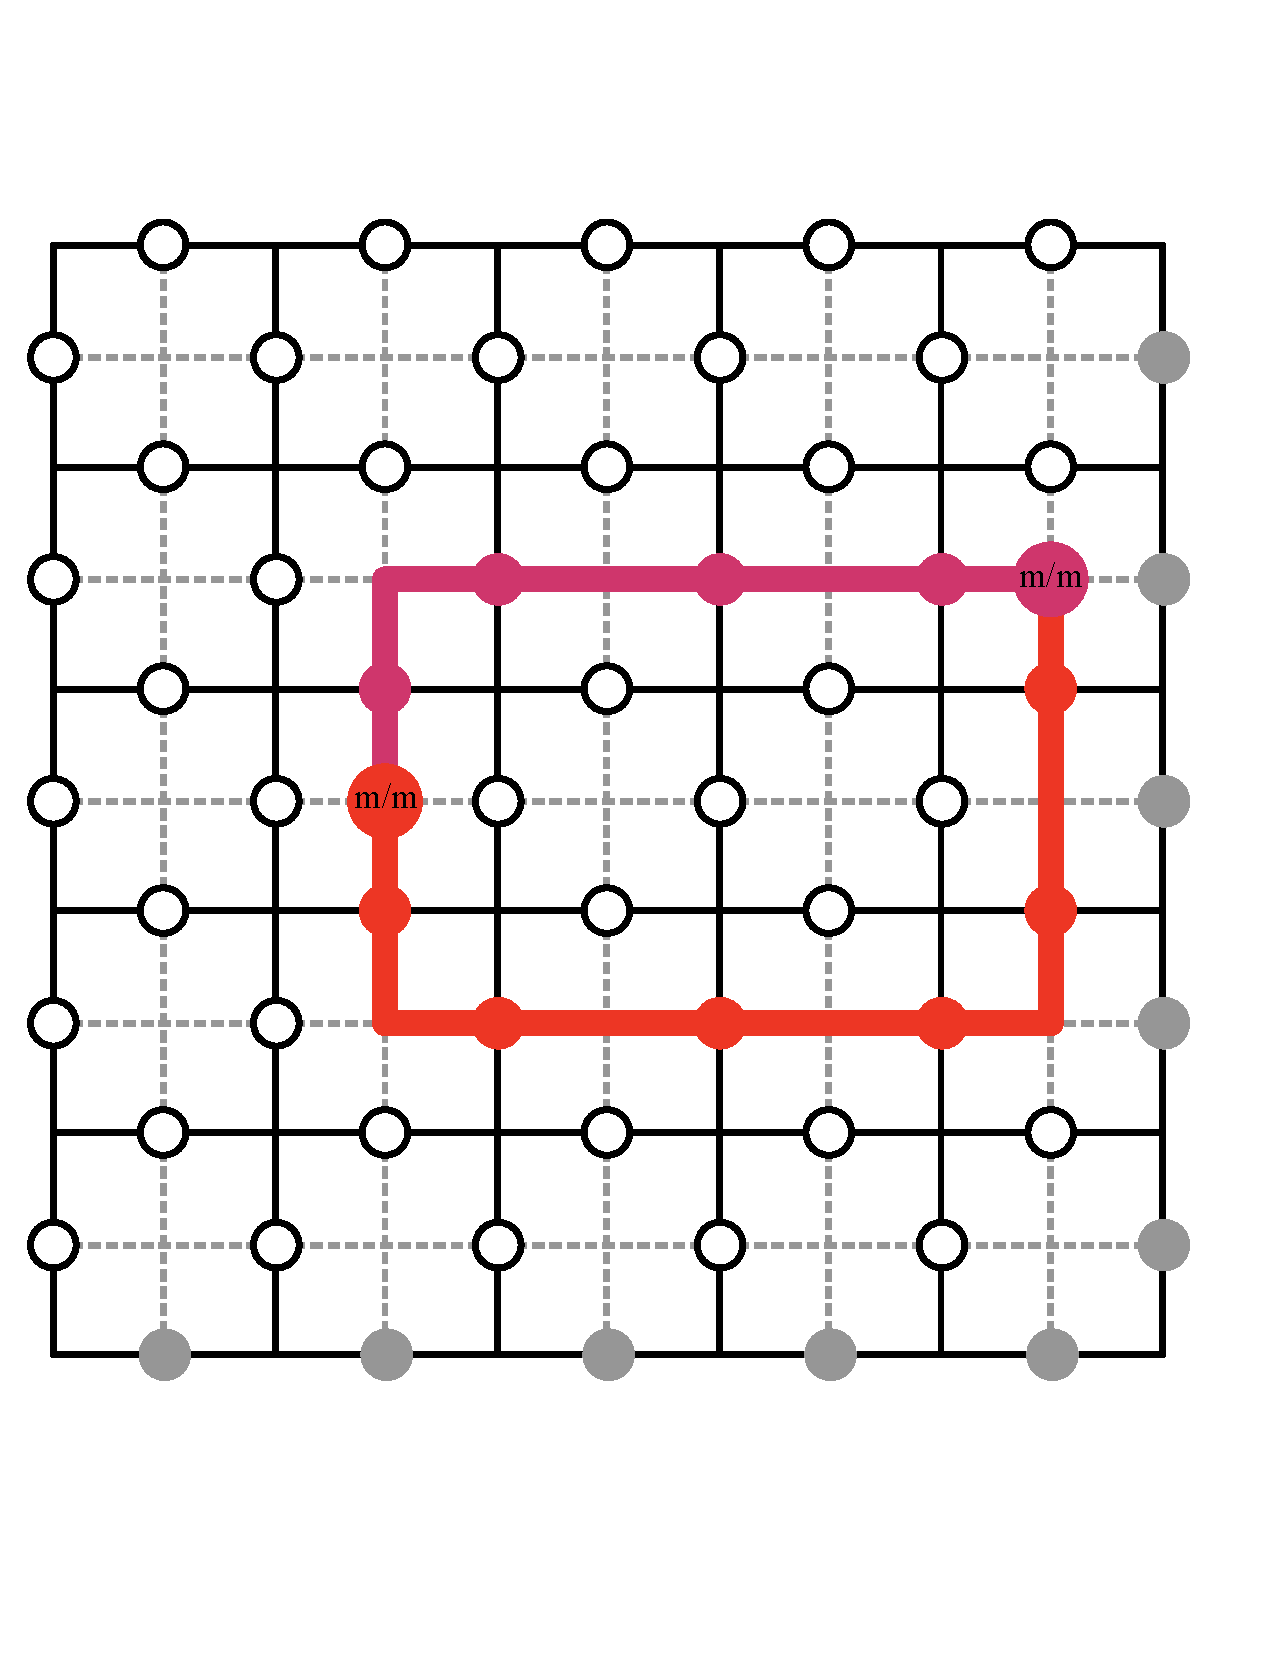
\includegraphics[width=\textwidth]{mfusion.pdf}
             \label{fig:fusion 1}
         \end{subfigure}
         \enspace\enspace\enspace
         \begin{subfigure}[b]{0.4\textwidth}
             \centering
             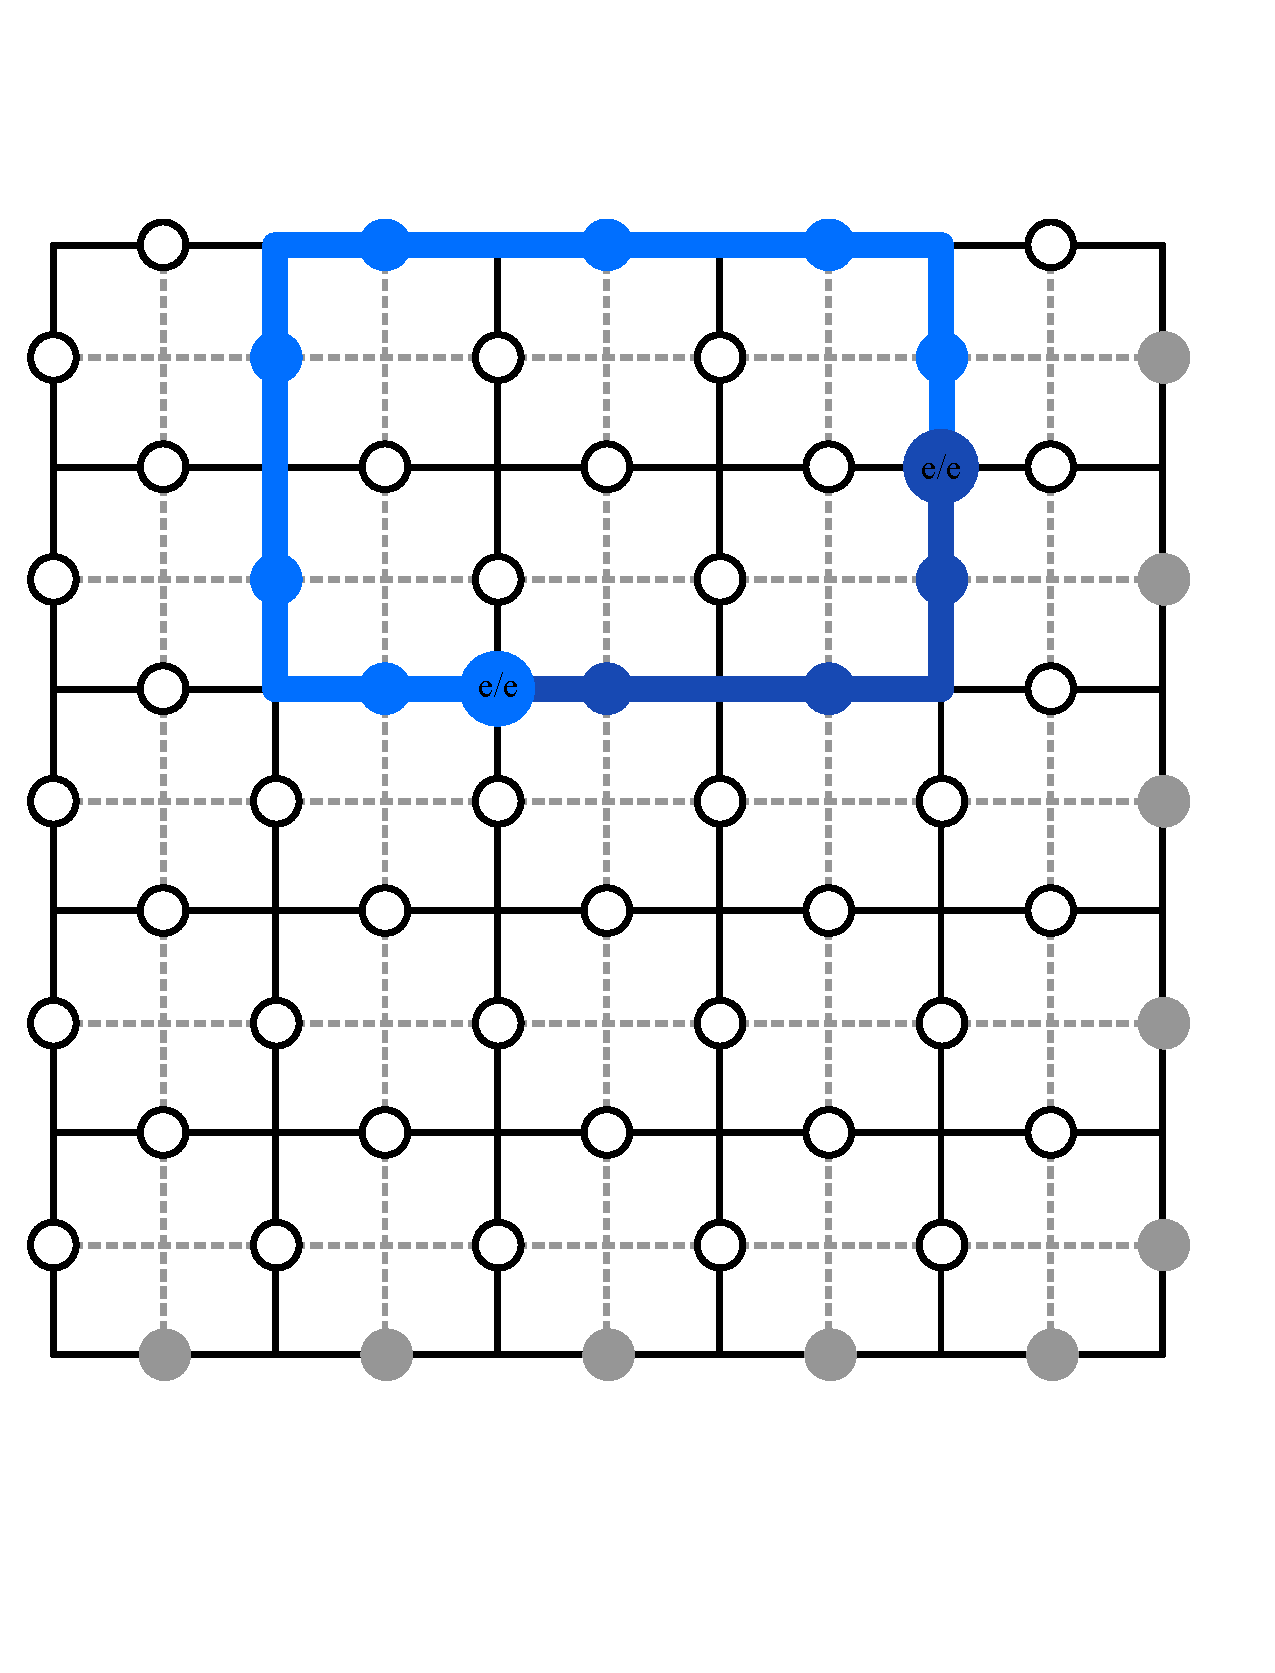
\includegraphics[width=\textwidth]{efusion.pdf}
             \label{fig:fusion 2}
         \end{subfigure}
            \caption{When a the same type of excitations are combined to form a closed loop (alternatively interpreted as transporting a quasiparticle to the site of its pair), the excitations are annihilated and the system is returned to the ground state as the topological defects are eliminated.}
            \label{fig:transport}
    \end{figure}

\newpage
\subsubsection{Deriving Fusion Rules} 
Fusion is the process through which quasiparticles are brought into proximity and combined to produce other quasiparticles. For a anyons $\{a_n\}_{n\in\{i,j,k\}}$, the fusion process is described as follows \cite{burnell2017}:
    \begin{align}
        a_i\times a_j=\sum_k N^k_{ij}a_k,
    \end{align}
where $N^k_{ij} = 1$ if $k\neq i\neq j$ and $N^k_{ij} = 0$ otherwise. We will show that the quasiparticles that arise in our toric code system behave as anyons by deriving their fusion rules and comparing them to $(67)$.\newline

First, we consider the fusion of quasiparticles of the same type. It has already been shown that transporting $e$ and $m$ quasiparticles to the site of their respective pairs returns the system to the vacuum state, implying $e\times e = m\times m = 1$, where $1$ is understood as the absence of quasiparticles, see Figure~\ref{fig:transport}. This reasoning extends to the dyon, as combining two dyons involves combining their respective electric and magnetic constituents, which will both annihilate. Therefore $\epsilon\times\epsilon = 1$. This reasoning suggests that $e$, $m$, and $\epsilon$ are their own antiparticles.\newline

We now consider the fusion of distinct quasiparticle types. By construction, dyons arise from the fusion of $e$ and $m$ quasiparticles, so $e\times m = \epsilon$. Furthermore, an $e$ quasiparticle is combined with an $\epsilon$ quasiparticle by transporting the free endpoint of the $\sigma^z$-type string (i.e. the endpoint that is not involved in the dyon) to the site of the dyon. The electric charges annihilate each other, causing the dyon to disappear, as the conditions required for its existence are no longer met. Thus, only the $\sigma^x$-type string operator remains. The same reasoning can be applied to the fusion of $m$ and $\epsilon$ quasiparticles, which results in the annihilation of the dyonic and magnetic quasiparticles, leaving behind the electric excitation. Therefore $\epsilon\times e = m$ and $\epsilon\times m = e$, or $N^\epsilon_{em} = N^e_{\epsilon m} = N^m_{\epsilon e} = 1$.\newline

The complete fusion rules for the system are therefore:
    \begin{align}
        e\times e = m\times m = \epsilon\times\epsilon = 1
    \end{align}
    \begin{align}
        e\times m = \epsilon,\enspace\enspace\enspace e\times\epsilon = m,\enspace\enspace\enspace m\times\epsilon = e.
    \end{align}
We can see that these fusion rules coincide with the anyonic behavior defined in $(67)$.

\subsubsection{Deriving Braiding Statistics}
The exchange statistics of anyons may be described by the function $\theta:\{1,e,m,\epsilon\}\rightarrow U(1)$, which represents the phase obtained when two identical anyons are exchanged \cite{ellison2022}. We will explicitly derive $\theta(a)$ for all $a\in\{e,m,\epsilon\}$.\newline

Consider two electric string operators $S^z(t)$ and $S^z(l)$ with $\partial_1t := \{v_0,v_n\}$ and $\partial_1l := \{v'_0,v'_n\}$ such that $t\cap l\neq\emptyset$ and $\partial_1t\cap\partial_1l := \emptyset$. These strings have four distinct endpoints, but intersect over some edges. For each $e\in t\cap l$, there are two superimposed $\sigma^z$ operators that cancel out, resulting in two new non-intersecting strings $S^z(t')$,$S^z(l')$ with $\partial_1t' := \{v_0,v'_n\}$ and $\partial_1l' := \{v'_0,v_n\}$, see Figure~\ref{fig:e exch}. It follows that no phase is incurred by the exchange and $\theta(e) = 1$. An equivalent argument can be made for $m$ quasiparticles to show that $\theta(m) = 1$. Electric charges and magnetic vortices therefore obey bosonic exchange statistics. The derivation of $\theta(\epsilon)$ is a bit more complex, and requires us to develop an understanding of braiding statistics.\newline
    \begin{figure}[h]
    \centering
    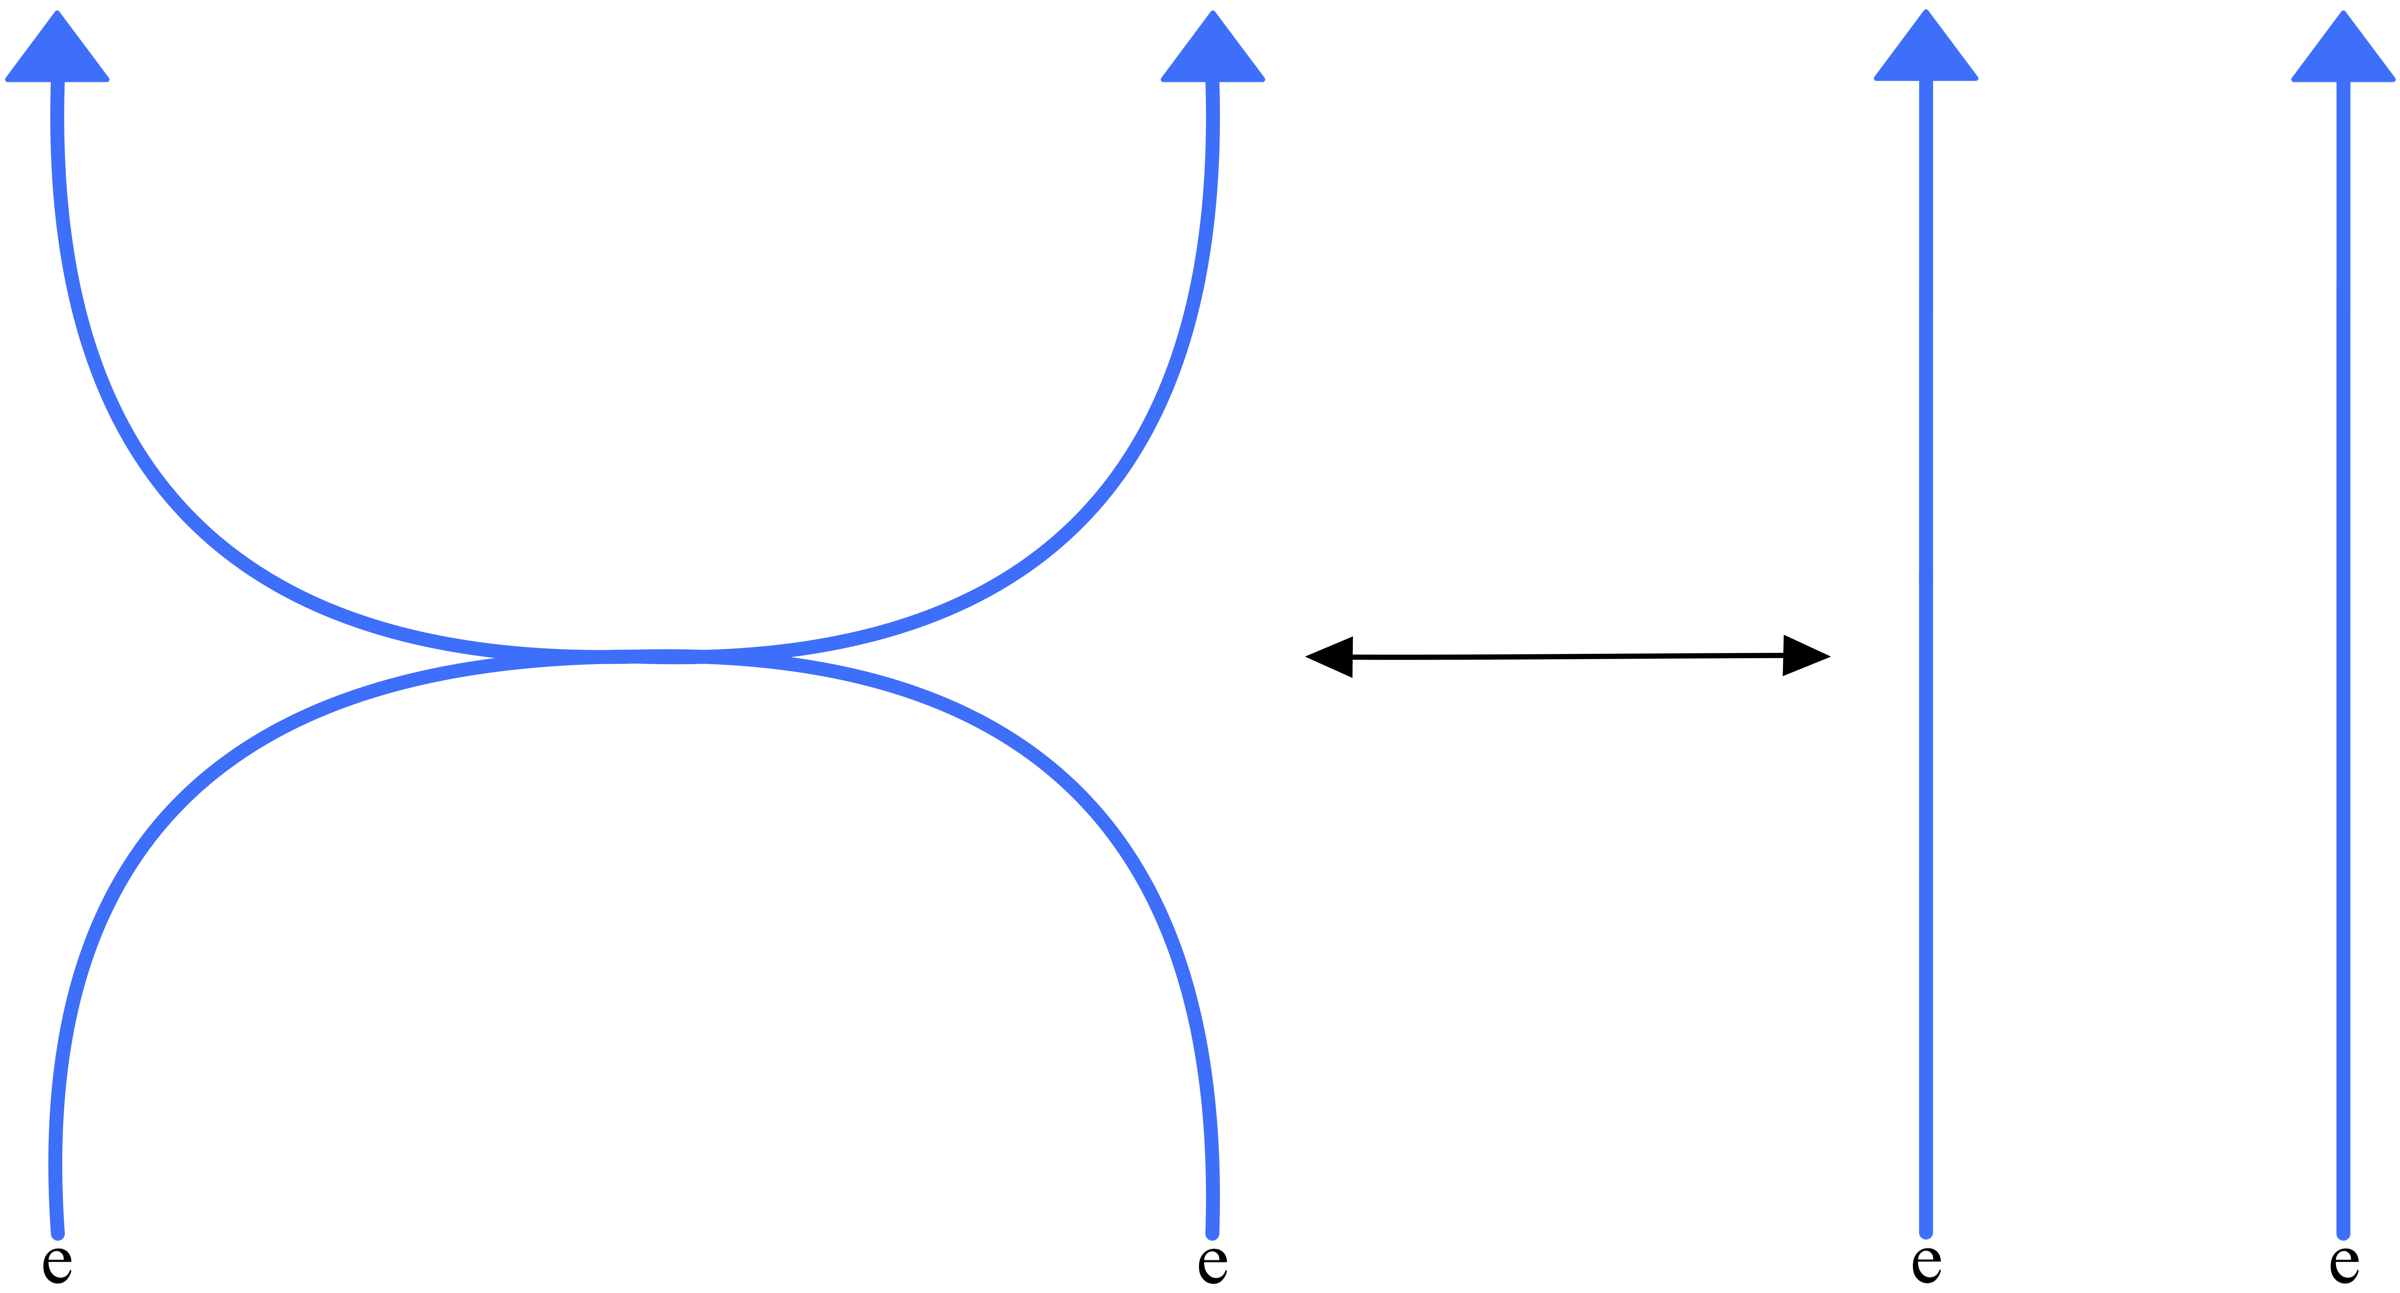
\includegraphics[width=0.4\textwidth]{ebraid.png}
    \caption{When $e$-type excitations are exchanged the superimposed sections cancel out, resulting in non-overlapping excitations (note: time flows upwards).}
    \label{fig:e exch}
    \end{figure}

Braiding is the process through which anyons are exchanged twice through time. This can also be thought of as moving one anyon around another in a full loop. This process is described by the function $B_\theta:\{e,m,\epsilon\}\times\{e,m,\epsilon\}\rightarrow U(1)$, where $B_\theta(a_1,a_1)$ represents the phase incurred when $a_1$ and $a_2$ are braided, for $a_1,a_2\in\{e,m,\epsilon\}$.\newline
    \begin{figure}[h]
    \centering
    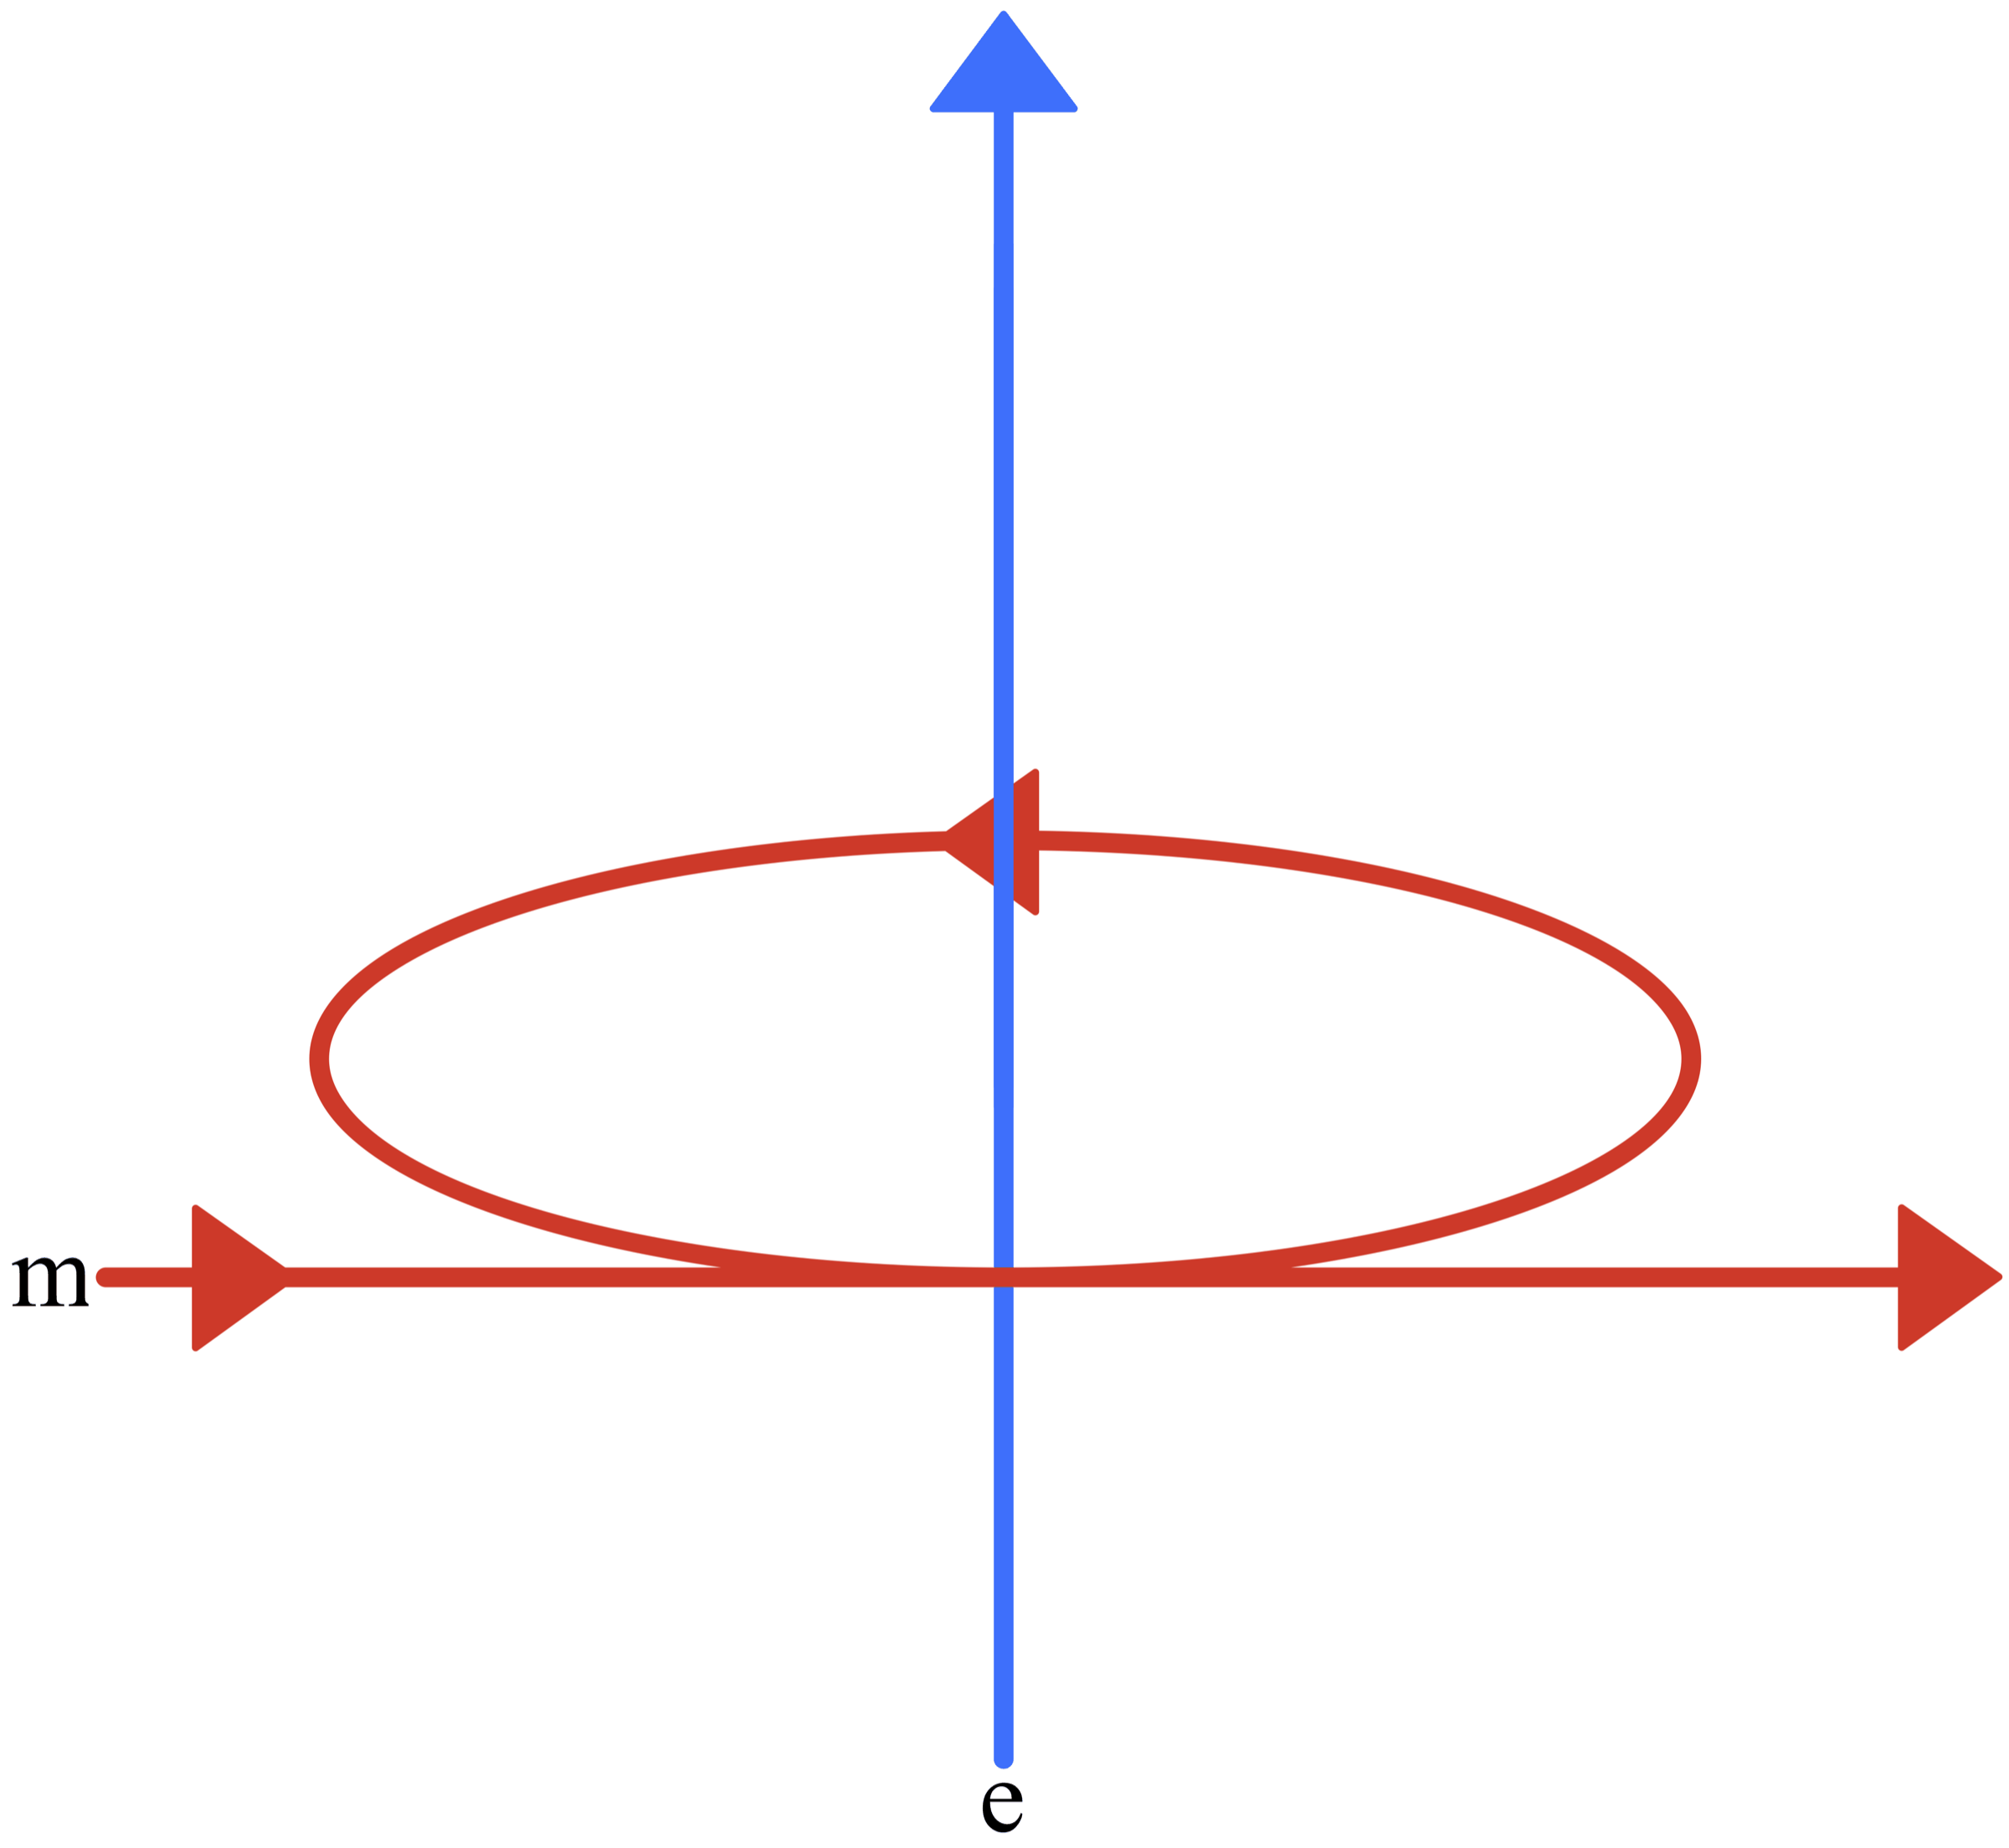
\includegraphics[width=0.4\textwidth]{braid.png}
    \caption{The braiding process of electric and magnetic quasiparticles.}
    \label{fig:x e exchange}
    \end{figure}

The phase factor $B_\theta(e,m)$ can be deduced by considering the effect of moving an $e$ quasiparticle around an $m$ quasiparticle in a full loop, as seen in Figure~\ref{fig:x e exchange}. Let $|\phi^{x,z}(t,t^*)\rangle = S^x(t^*)S^z(t)|\psi\rangle$ represent a state with both types of excitations. Without loss of generality, we assume that an $e$ quasiparticles occurs on vertex $v_0\in V$ and an $m$ quasiparticle exists on plaquette $p_0\in P$; furthermore, we assume that this configuration does not satisfy the conditions required for a dyon. We transport the $e$ quasiparticle around the $m$ quasiparticle by applying $S^z(\gamma)$ where $\gamma$ is a closed $1$-chain beginning and ending on $v_0$:
    \begin{align}
        S^z(\gamma)|\phi^{x,z}\rangle &= \prod_{e\in\gamma}\sigma^z_e|\phi^{x,z}\rangle.
    \end{align}
Since $\partial_1\gamma = 0$, then $\gamma = \partial_2\Pi$ for some connected collection of plaquettes $\Pi\subseteq P$. As such, the action of $S^z(\gamma)$ can be identified with a group of operators $\{B_p\}_{p\in\Pi}$. Thus:
    \begin{align}
        S^z(\gamma)|\phi^{x,z}\rangle &= \prod_{p\in\Pi}B_p|\phi^{x,z}\rangle.
    \end{align}
        \begin{figure}[h]
    \centering
    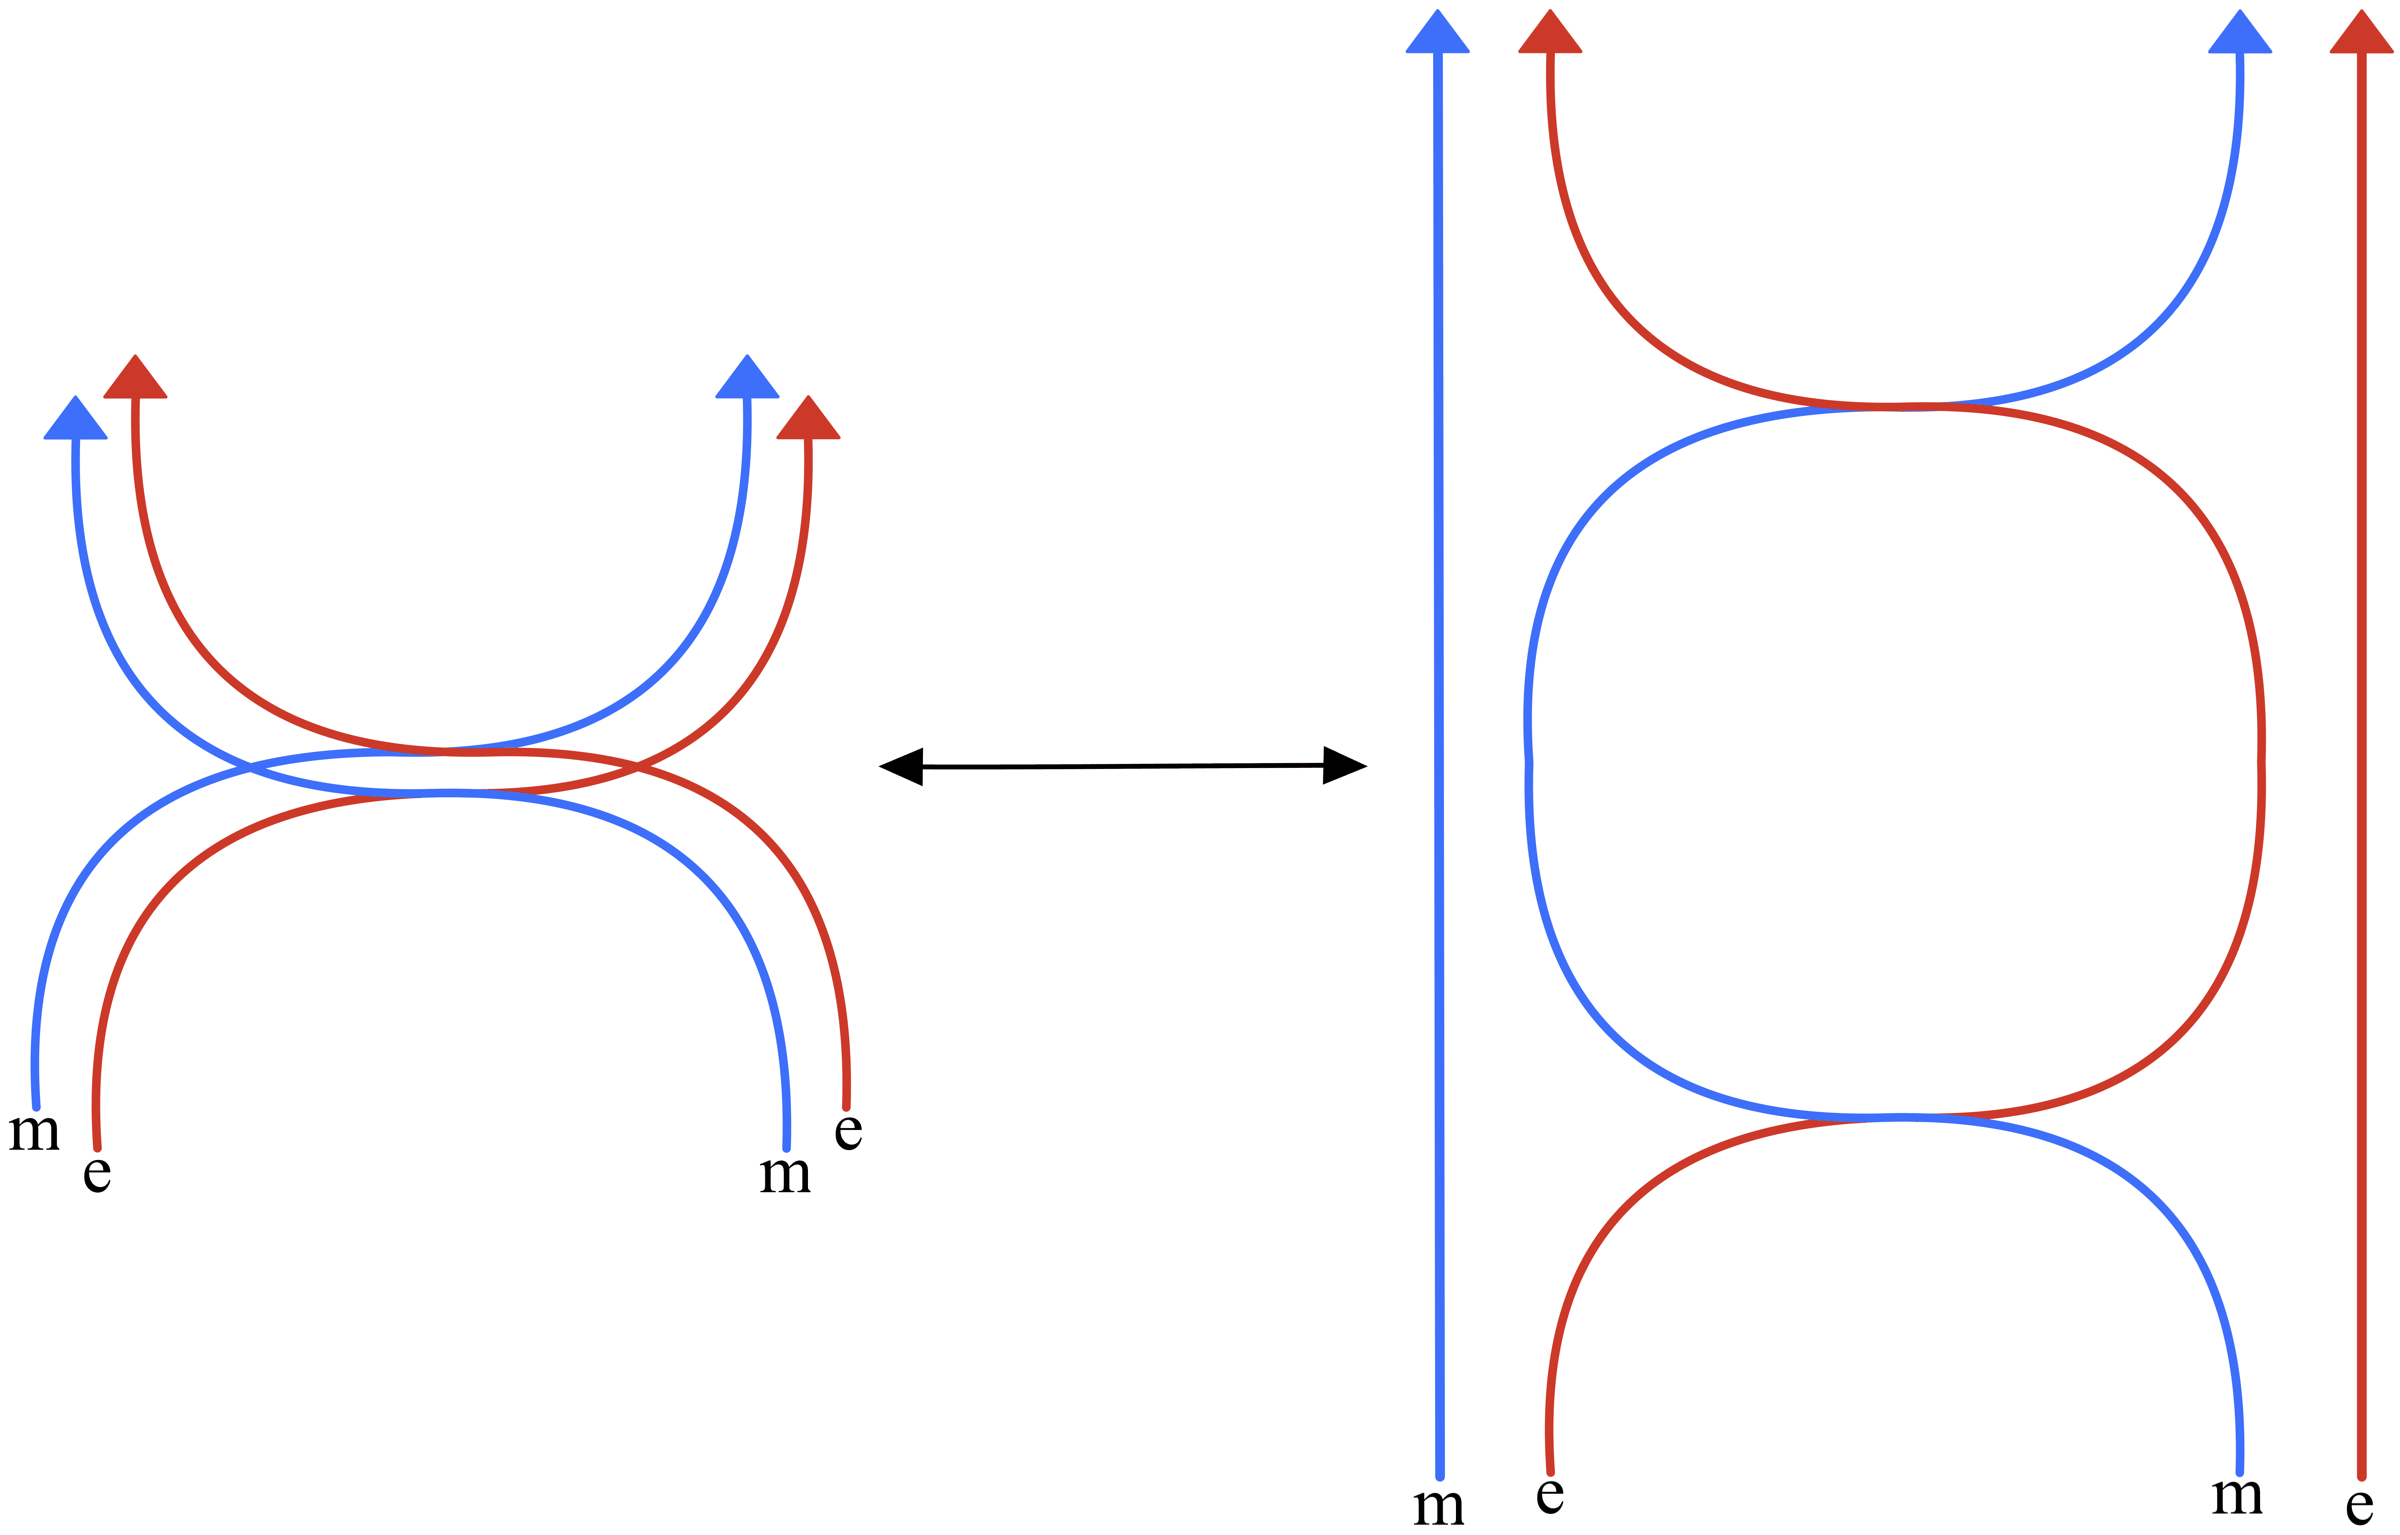
\includegraphics[width=0.4\textwidth]{dyonbraid.png}
    \caption{The exchange statistics of a dyon.}
    \label{fig:dyon exch}
    \end{figure}
Noting that $p_0\in\Pi$, and therefore $B_{p_0}|\phi^{x,z}\rangle = -B_{p_0}|\phi^{x,z}\rangle$, we finally obtain:
    \begin{align}
        S^z(\gamma)|\phi^{x,z}\rangle &= -|\phi^{x,z}\rangle.
    \end{align}
This implies that $B_\theta(e,m) = -1$. \newpage

There is a general relationship between the braiding phase $B_\theta$ and the self-exchange phase $\theta$ \cite{ellison2022}:
    \begin{align}
        B_\theta(a_1,a_2) = \frac{\theta(a_1\times a_2)}{\theta(a_1)\theta(a_2)},
    \end{align}
for $a_1,a_2\in\{e,m,\epsilon\}$. We can use equation ($73$), as well as our explicitly derived value for $B_\theta(e,m)$, to derive the self-exchange phase factor for the dyon: 
    \begin{align}
        B_\theta(e,m) &= \frac{\theta(e\times m)}{\theta(e)\theta(m)}\\
        B_\theta(e,m)\theta(e)\theta(m) &= \theta(\epsilon)\\
        B_\theta(e,m) &= \theta(\epsilon).
    \end{align}
We find that exchanging two dyons picks up the same phase as braiding $e$ and $m$ particles, and so $\theta(\epsilon) = -1 $, which can be seen graphically in Figure~\ref{fig:dyon exch} Finally, we may compute $B_\theta(e,\epsilon)$ and $B_\theta(m,\epsilon)$:
    \begin{align}
        B_\theta(e,\epsilon) &= \frac{\theta(e\times\epsilon)}{\theta(e)\theta(\epsilon)}\\
        &= \frac{\theta(m)}{\theta(e)\theta(\epsilon)}\\
        &= -1\\
        B_\theta(m,\epsilon) &= \frac{\theta(m\times\epsilon)}{\theta(m)\theta(\epsilon)}\\
        &= \frac{\theta(e)}{\theta(m)\theta(\epsilon)}\\
        &= -1
    \end{align}
Finally, the complete set of exchange and braiding statistics may be summarized as follows:
    \begin{align}
        \theta(e) = \theta(m) = 1,\enspace\enspace\enspace\theta(\epsilon) = -1\\
        B_\theta(e,m) = B_\theta(e,\epsilon) = B_\theta(m,\epsilon) = -1.
    \end{align}
We therefore see that $e$ and $m$ have bosonic statistics, whereas $\epsilon$ has fermionic statistics. 

\subsection{Toric Code with Boundaries}
Smooth manifolds such as the torus are conveniently simple to conceptualize theoretically. However, as we have seen, this straightforward structure yields uninteresting encoded logical operators. As such, non-trivial topologies are required to construct and implement more exotic logical gates \cite{cheipesh2019}. Although this comes at the risk of complicating the situation from a geometrical point of view, it turns out that we can use boundaries to construct these non-trivial topologies without excessively distorting the formalism we have developed.\newline

In two dimensions, the toric code admits two types of boundaries, which are referred to as rough and smooth. We may formalize the notion of boundaries on a two-dimensional square lattice $\mathcal{L}$ as follows:
    \begin{align}
        \partial\mathcal{L} = \bigcup^4_{i = 1}\partial\mathcal{L}^i
    \end{align}
Rough boundaries consist of open edges, meaning that they are exclusively comprised of vertices, and therefore serve as endpoints of $e$-type excitations. Conversely, smooth boundaries allow for the endpoints of $m$-type excitations. We will use $\partial\mathcal{L}^r$, $\partial\mathcal{L}^s$ to denote rough and smooth boundaries, respectively (Figure~\ref{fig:strings on mixed boundaries}). It is easy to see that strings with both endpoints terminating on the same boundary are homologically trivial. A toric code defined on a lattice with entirely smooth or entirely rough boundaries contains no homologically non-trivial cycles, and therefore encodes no qubits \cite{ellison2022, hastings2021}. However, lattices with mixed boundaries can encode a finite number of qubits.
    \begin{figure}[h]
         \centering
         \begin{subfigure}[b]{0.4\textwidth}
             \centering
             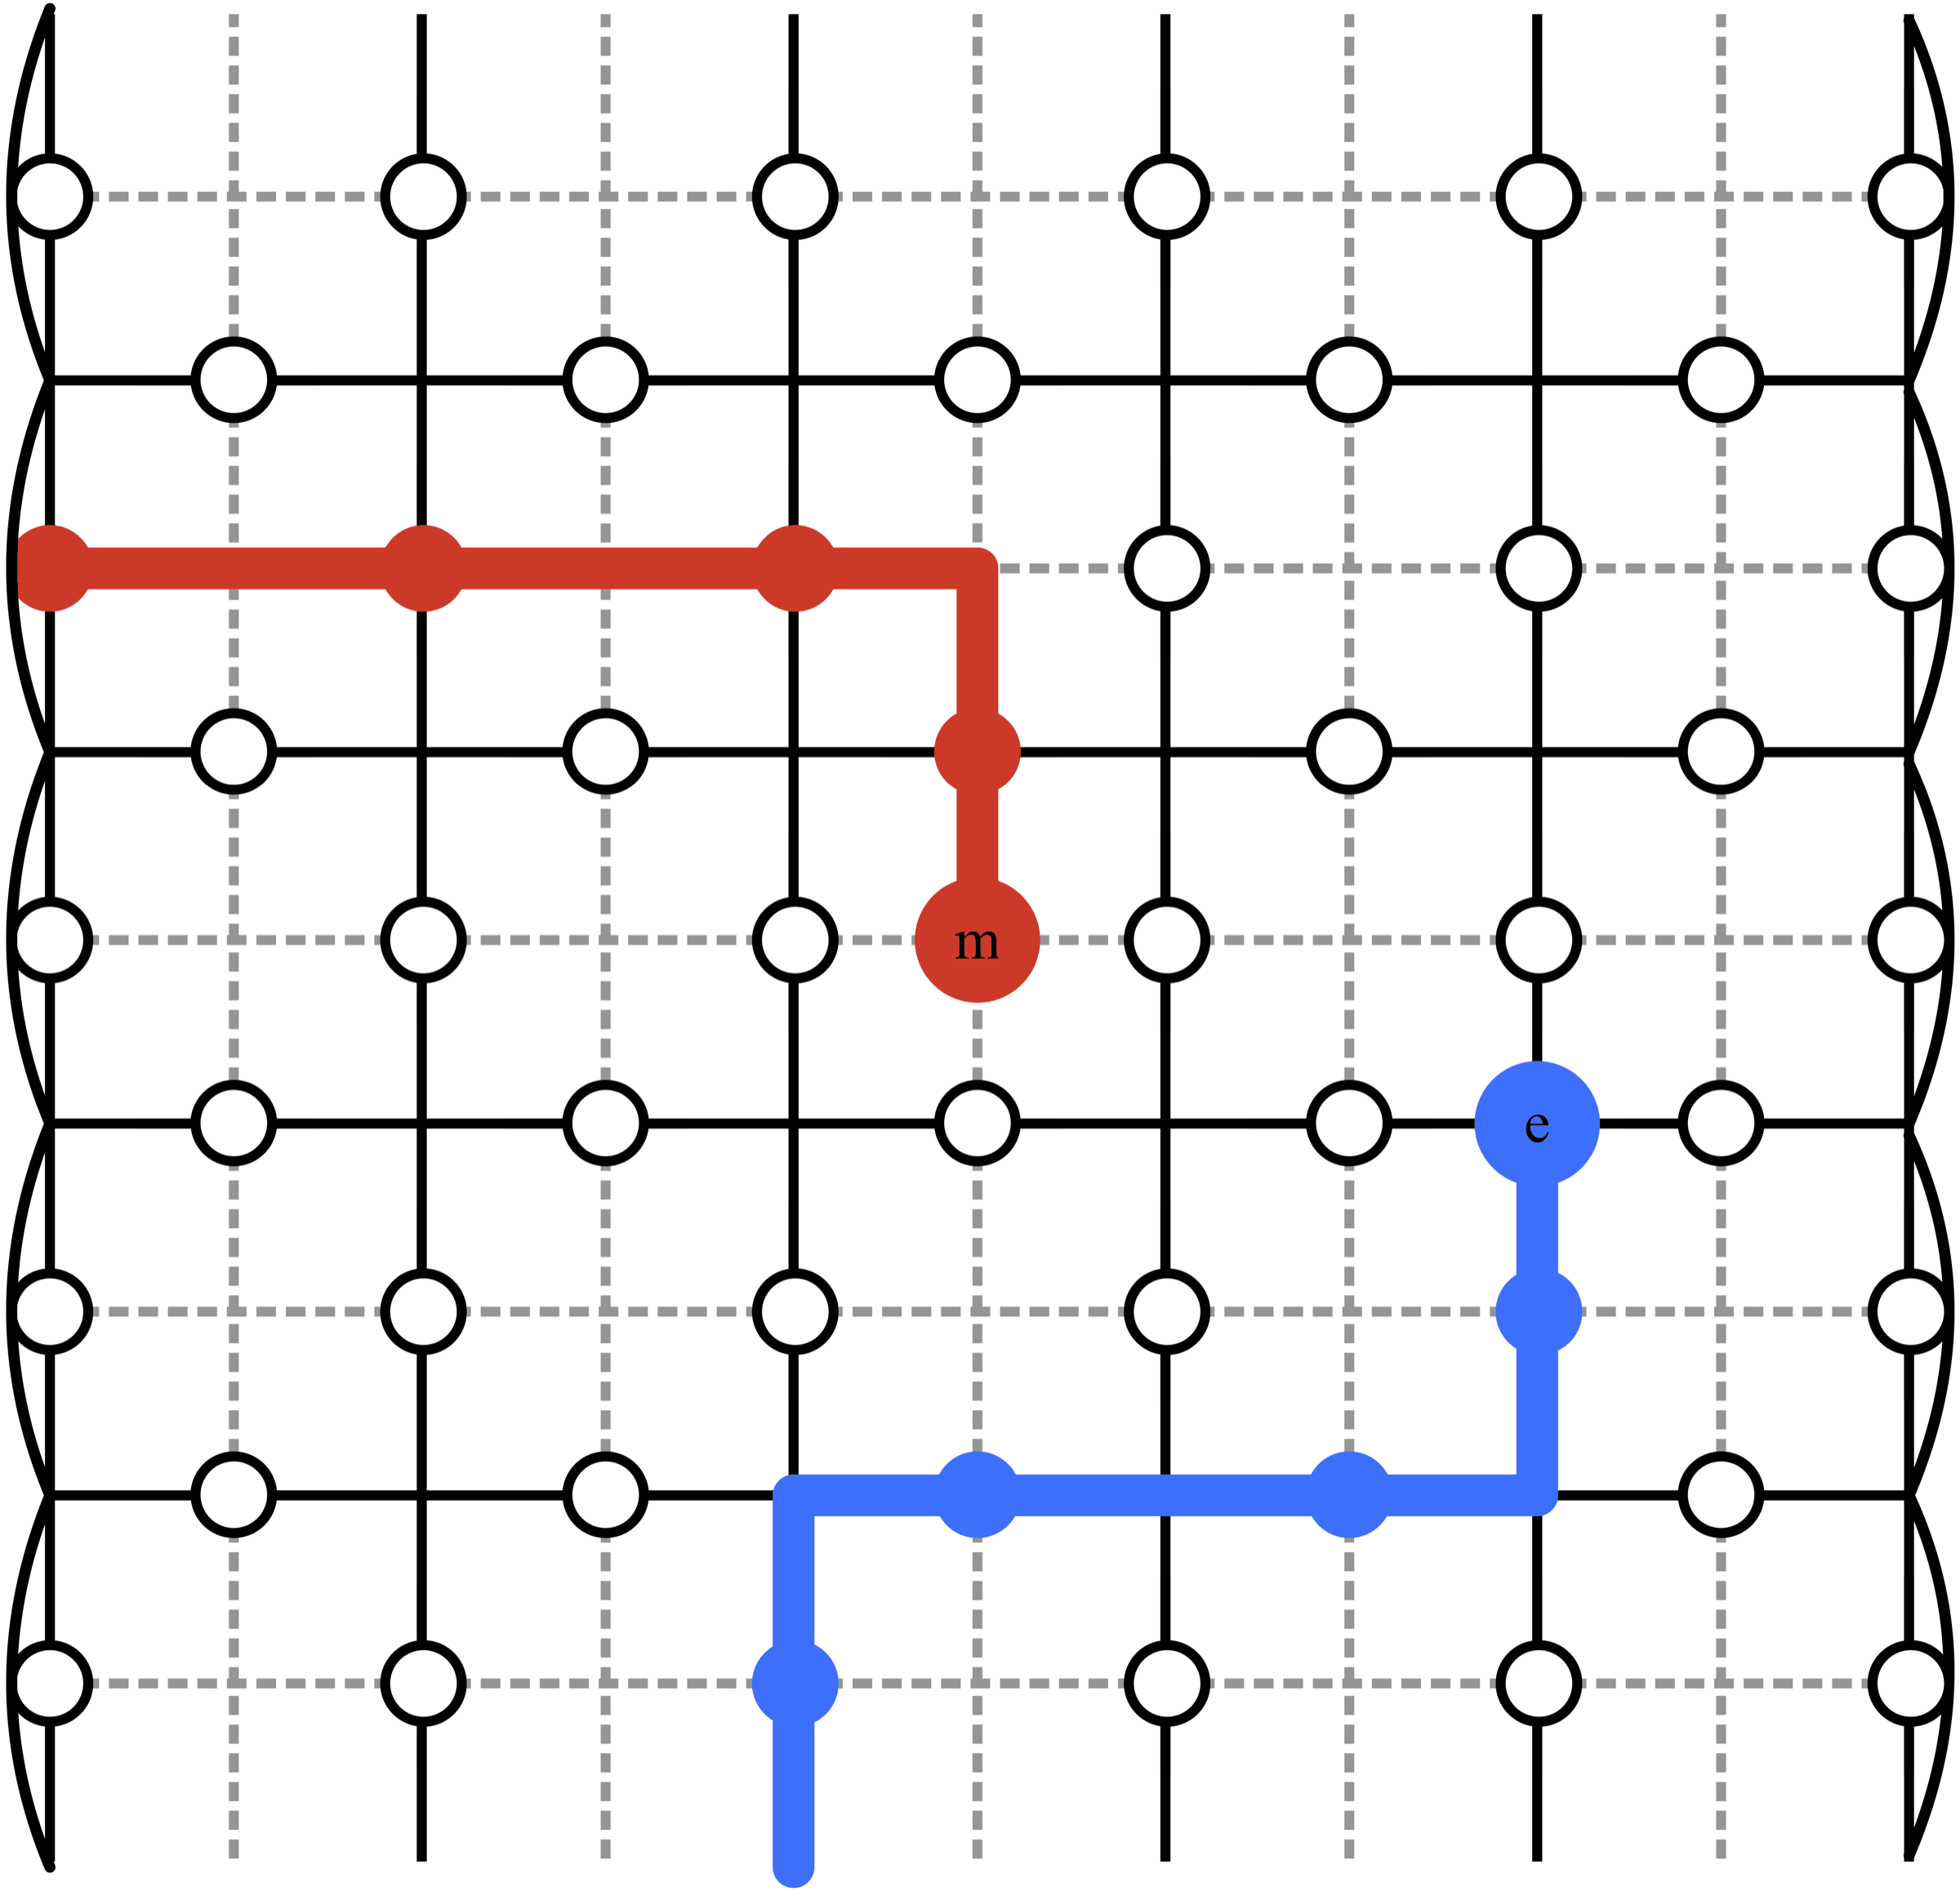
\includegraphics[width=\textwidth]{boundstr.png}
             \caption{Rough boundaries serve as endpoints of electric excitations, and smooth boundaries serve as endpoints of magnetic excitations.}
             \label{fig:strings on mixed boundaries}
         \end{subfigure}
         \enspace\enspace\enspace
         \begin{subfigure}[b]{0.4\textwidth}
             \centering
             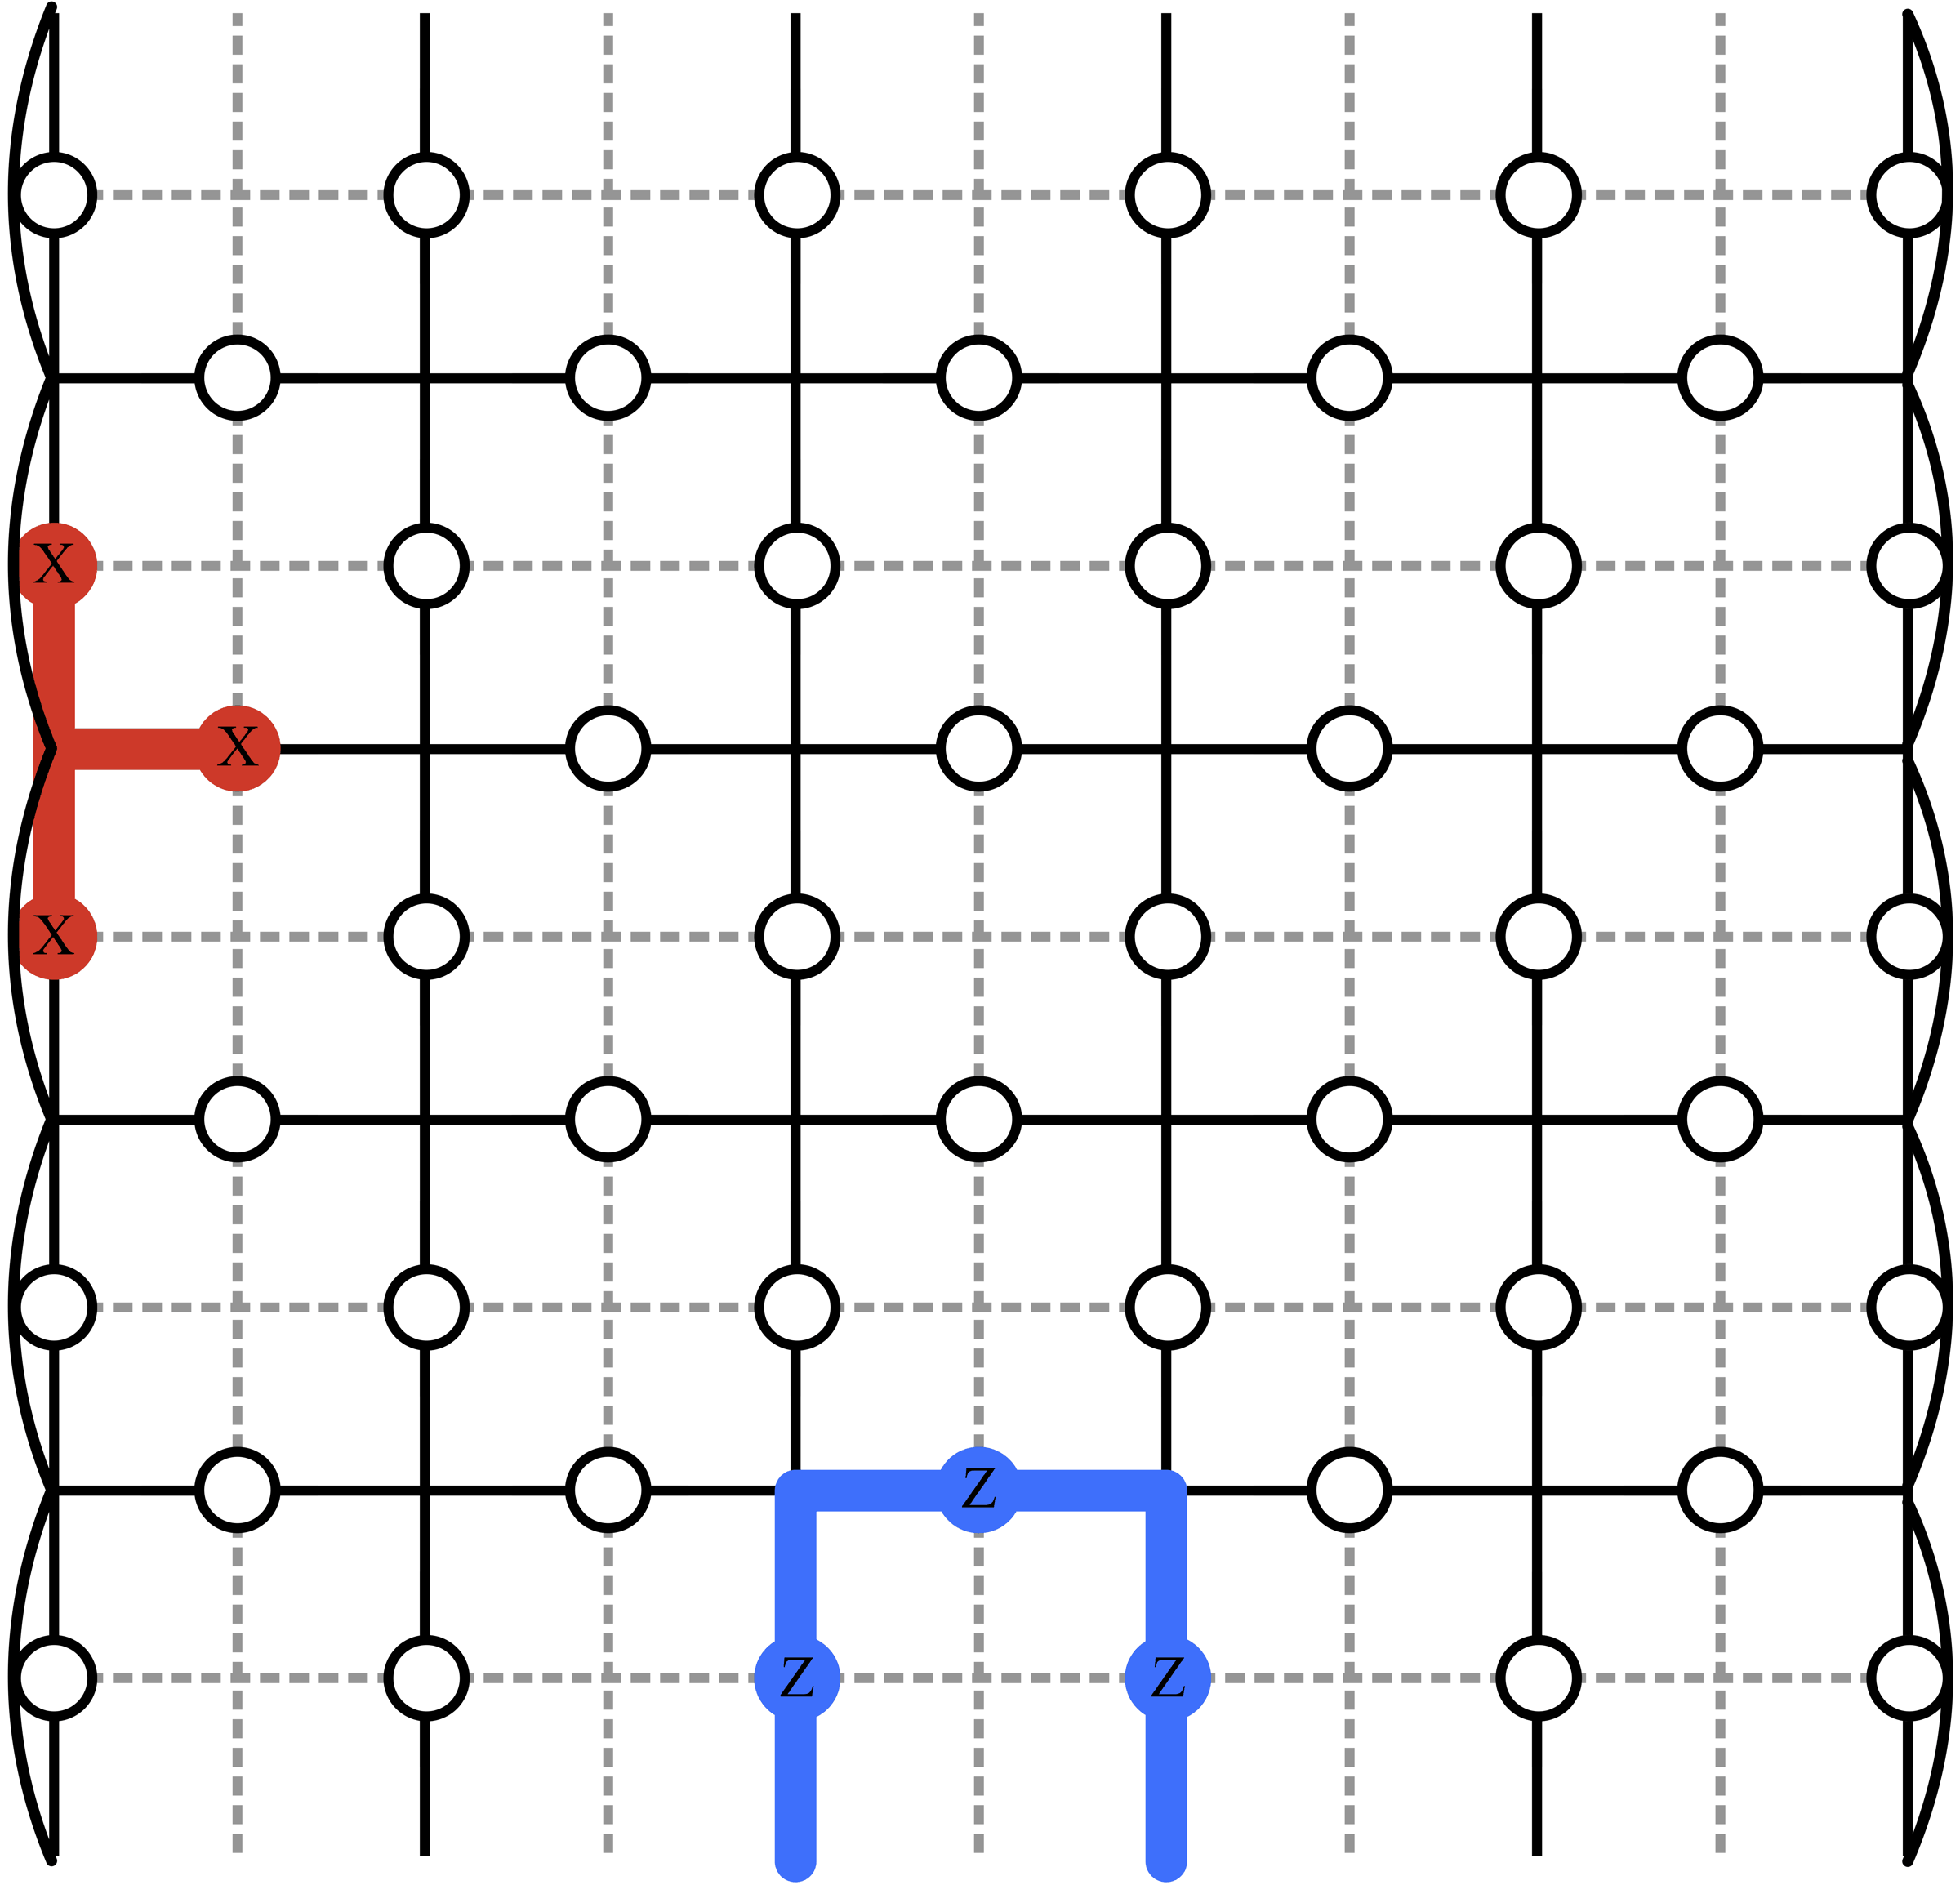
\includegraphics[width=\textwidth]{modop.png}
             \caption{Stabilizer operators are modified to weight-three on boundaries.\newline\newline}
             \label{fig:modified stabilizers}
         \end{subfigure}
            \caption{Lattice with two rough boundaries (top \& bottom) and two smooth boundaries (left \& right).}
            \label{fig:boundaries}
    \end{figure}

Stabilizer operators need to be modified along the boundaries. On rough boundaries, plaquette operators become weight-three (meaning they act on three edges instead of four). Similarly, vertex operators become weight-three on smooth boundaries. We will take $A'_v$ and $B'_p$ to be the modified weight-three vertex and plaquette operators, respectively. We define the following modified sets of vertices and plaquettes along the boundaries:
    \begin{align}
        V_s &:= \{v\in V|v\in\partial_1e\enspace\text{for}\enspace e\in\partial\mathcal{L}^s\}\\
        V_r &:= \{v\in V|v\in\partial_1e\enspace\text{for}\enspace e\in\partial\mathcal{L}^r\}\\
        P_s &:= \{p\in P|\exists e\in\partial_2p\enspace\text{where}\enspace e\in\partial\mathcal{L}^s\}\\
        P_r &:= \{p\in P|\exists e\in\partial_2p\enspace\text{where}\enspace e\in\partial\mathcal{L}^r\}
    \end{align}
We can therefore define interior vertices and plaquettes:
    \begin{align}
        V_{int} = (V_s\cup V_r)^c\\
        P_{int} = (P_s\cup P_r)^c
    \end{align}
Along rough and smooth boundaries, the Hamiltonian is defined:
    \begin{align}
        H^{s}_{TC} &= -\sum_{v\in V_s}A'_v-\sum_{p\in P_s}B_p\\
        H^{r}_{TC} &= -\sum_{p\in P_r}B'_p,
    \end{align}
where $H^s_{TC}$ and $H^r_{TC}$ denote the Hamiltonian along rough and smooth boundaries, respectively. Consider a toric code defined on a lattice $\mathcal{L}$ with two smooth and two rough boundaries. The Hamiltonian of $\mathcal{L}$ is defined:
    \begin{align}
        H_{TC} = -\sum_{v\in V_{int}}A_v-\sum_{v'\in V_s}A'_{v'}-\sum_{p\in P_{int}\cup P_s}B_p-\sum_{p'\in P_r}B'_{p'}
    \end{align}

\newpage
\subsubsection{Quasiparticle Condensation at Boundaries}
In the toric code with boundaries, the modified Hamiltonian results in a very interesting phenomenon on the boundaries, known as \emph{quasiparticle condensation}\cite{burnell2017}. Recall that excitations are the manifestation of topological defects, which arise when the eigenvalues of the stabilizers are modified. In other words, string operators create defects because their endpoints do not commute with $H_{TC}$. Throughout this section we will work with a toric code defined on a square lattice $\Lambda$ with two rough and two smooth boundaries, where opposite boundaries are of the same type. This toric code encodes one qubit.
\newline

Consider a $\sigma^z$-type string operator $S^z(t)$ on the toric code with alternating boundaries, with one endpoint in the interior of the lattice and the other on a rough boundary - so $\partial_1t := \{v_0,v_1\}$ with $v_0\in V_{int}$ and $v_1\in V_r$. As discussed earlier, the interior endpoint $v_0$ represents a topological defect because it anti-commutes with $A_{v_0}$. However, due to the modified stabilizer structure of the system, it is impossible to place a vertex operator at $v_1$. Consequently, the string operator commutes with the modified Hamiltonian at $v_1$, implying that there is no energy cost for the $e$-type quasiparticle’s existence on the rough boundary. Due to this phenomenon, we say that electric quasiparticles \emph{condense} on rough boundaries. An equivalent argument shows that magnetic quasiparticles condense on smooth boundaries.\newline

This condensation mechanism ensures that logical operators do not create topological defects on boundaries, preserving the code’s integrity. Instead, they enable the transportation of virtual excitations between boundaries, a process that preserves the ground state (due to the lack of energy cost) but applies the logical transformations required for quantum computation. Therefore, in a mixed boundary system, logical string operators act as processes that transport a single $e$-type or $m$-type excitation across the lattice without creating topological defect. For example, a $\overline{Z}_{1,2}$ logical operator can be interpreted as creating a single $e$-type excitation at one rough boundary, transporting it across the lattice, and then absorbing it at the opposite rough boundary. Similarly, the $\overline{X}$ logical operator creates an $m$-type excitation at a smooth boundary, transports it across the lattice, and then absorbs it at the opposite smooth boundary at no energy cost.\newline

Logical operators can be continuously deformed without altering their effect on the encoded qubits, as long as they connect appropriate boundary types. For instance, a $\overline{Z}$ logical operator, which transports $e$-type excitations, may take any path between any two rough boundaries without changing its effect on the encoded qubit. The logical action depends solely on the type of boundary between which it operates, not on the specific path it takes along the lattice. This freedom in the deformation of logical string operators reflects the topological nature of the code, where information is stored in the global connectivity of the paths rather than their precise local form. The commutation relations between logical operators are assured by the braiding statistics of the $e$ and $m$ excitations as they are transported between boundaries.
    \begin{figure}[h]
         \centering
         \begin{subfigure}[b]{0.4\textwidth}
             \centering
             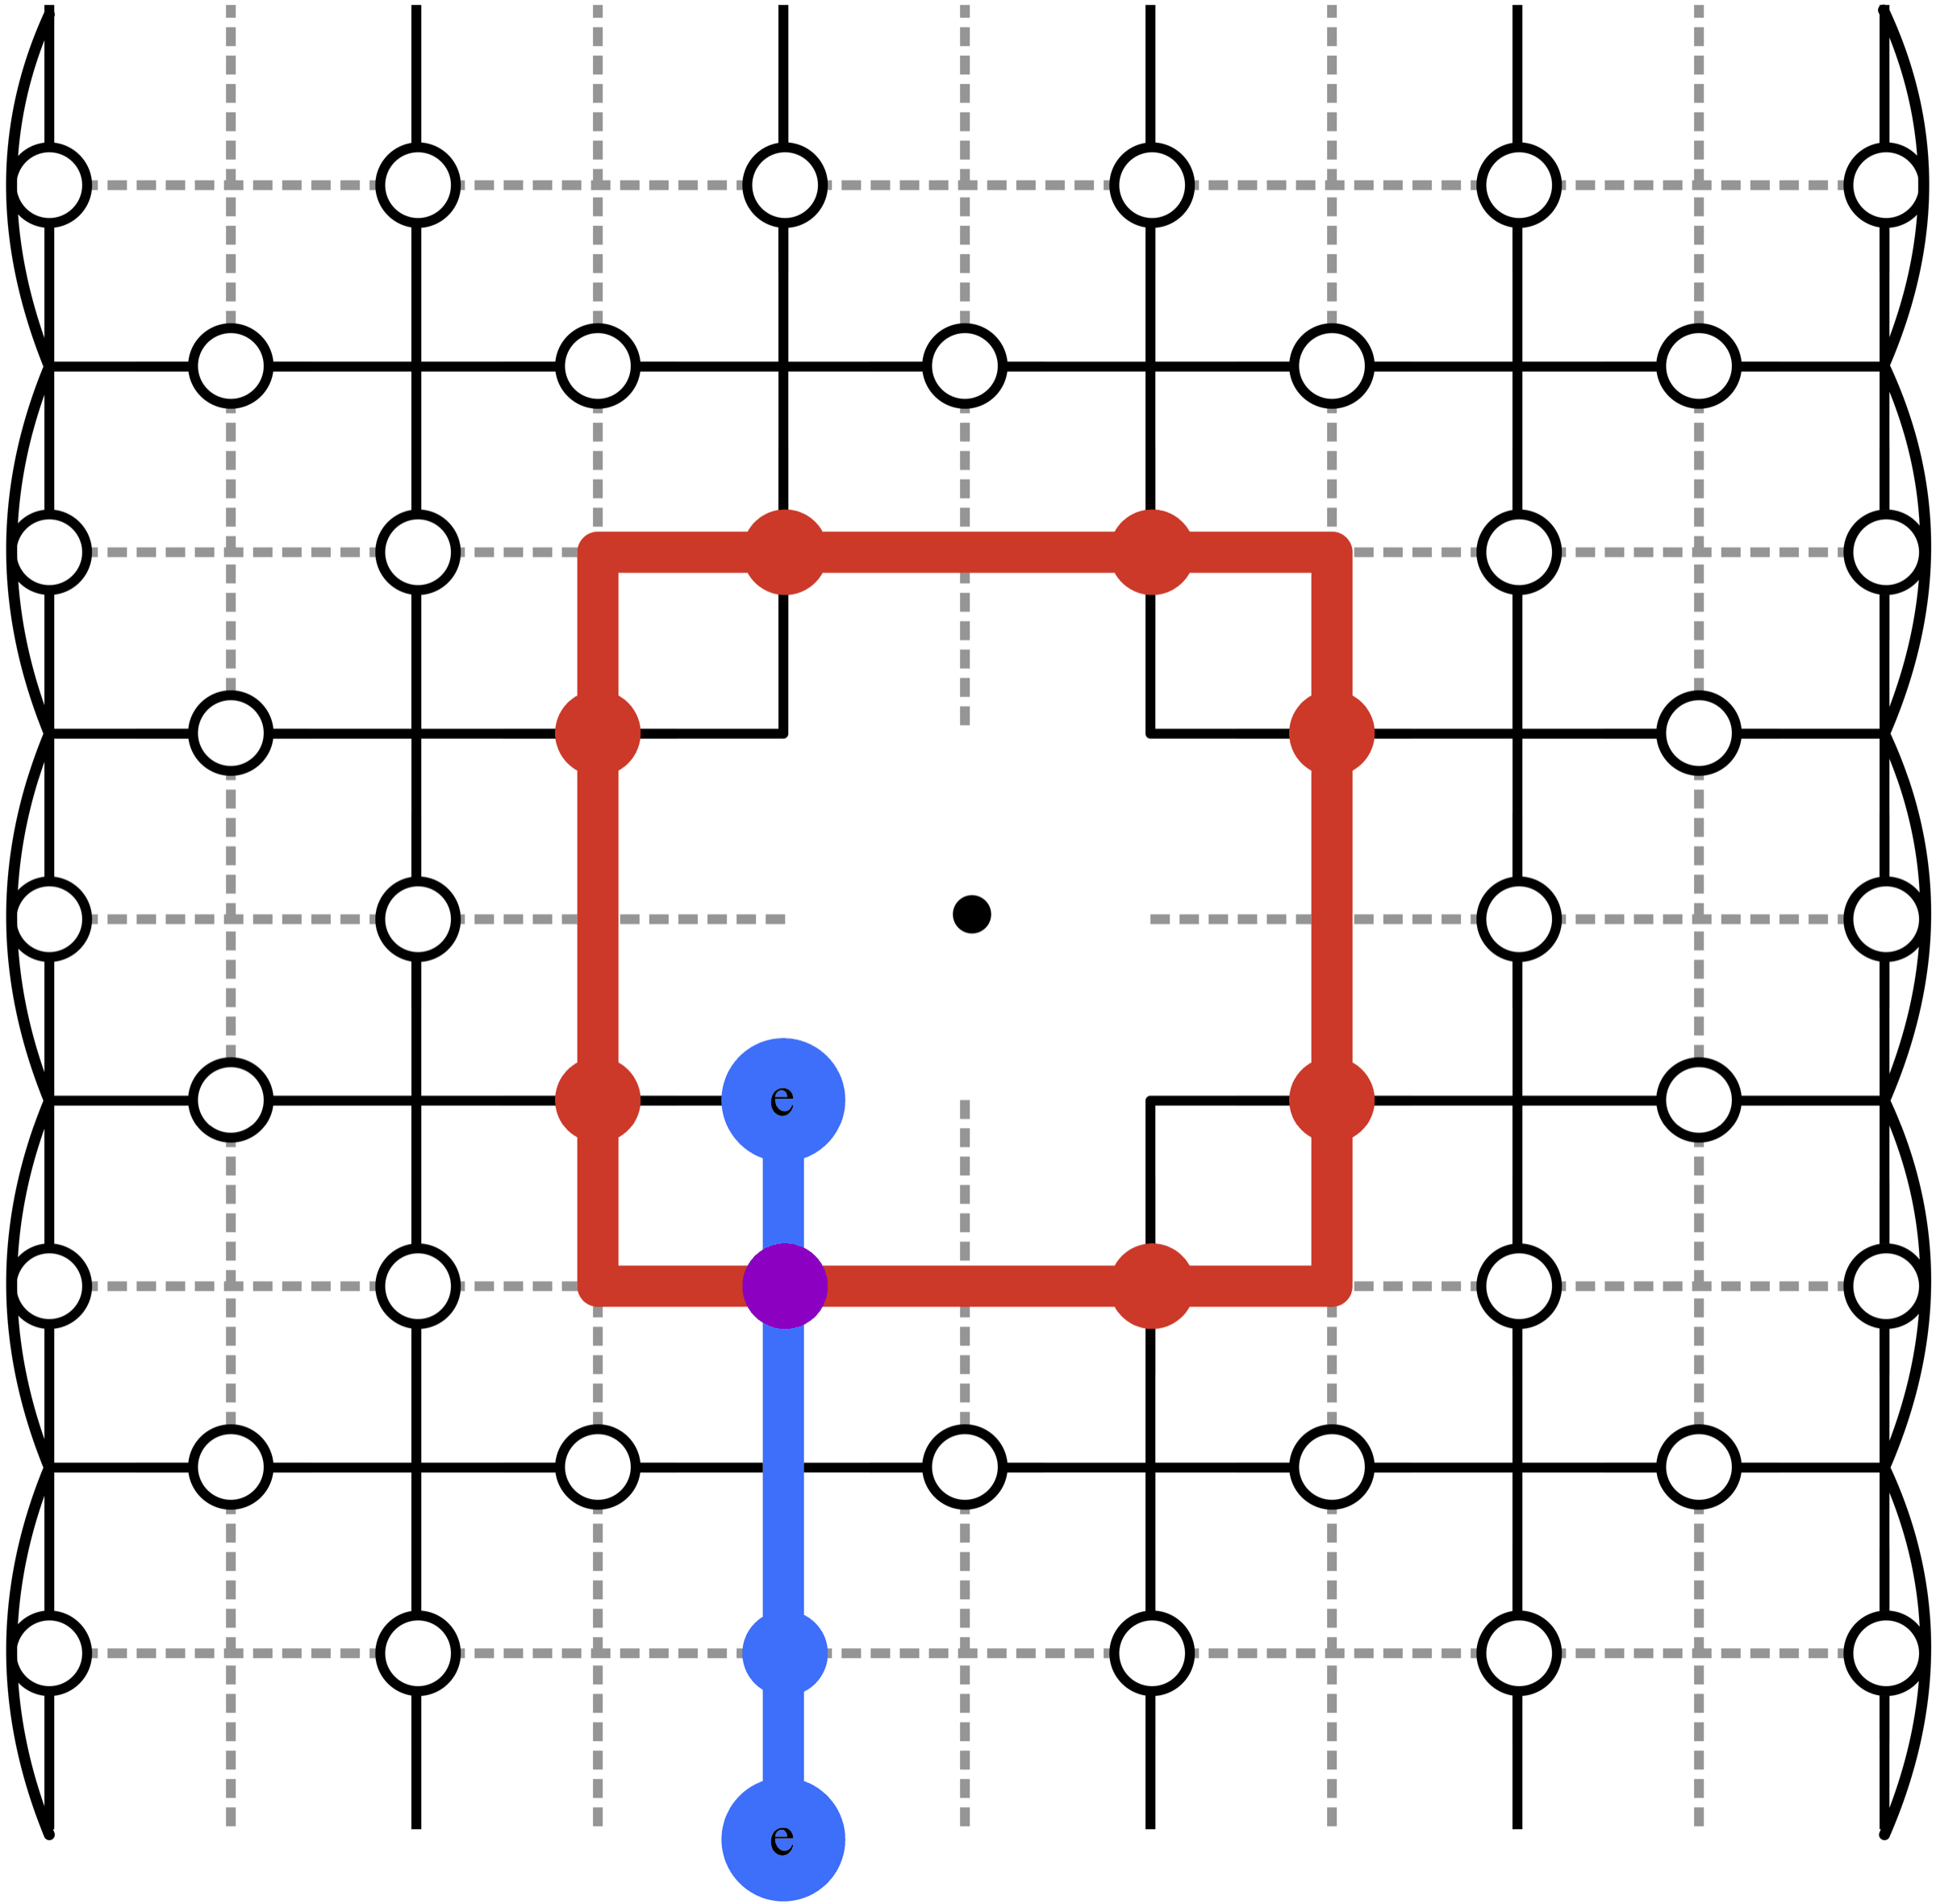
\includegraphics[width=\textwidth]{plaqpunct.png}
             \caption{When a plaquette is removed, a rough boundary is created in the interior of the lattice. New logical operators may be constructed; one as a closed loop of $\sigma^x$ operators enclosing the puncture, and one as a string of $\sigma^z$ operators connecting the boundary of the puncture to another rough boundary.\newline\newline\newline}
             \label{fig:face puncture}
         \end{subfigure}
         \enspace\enspace\enspace
         \begin{subfigure}[b]{0.4\textwidth}
             \centering
             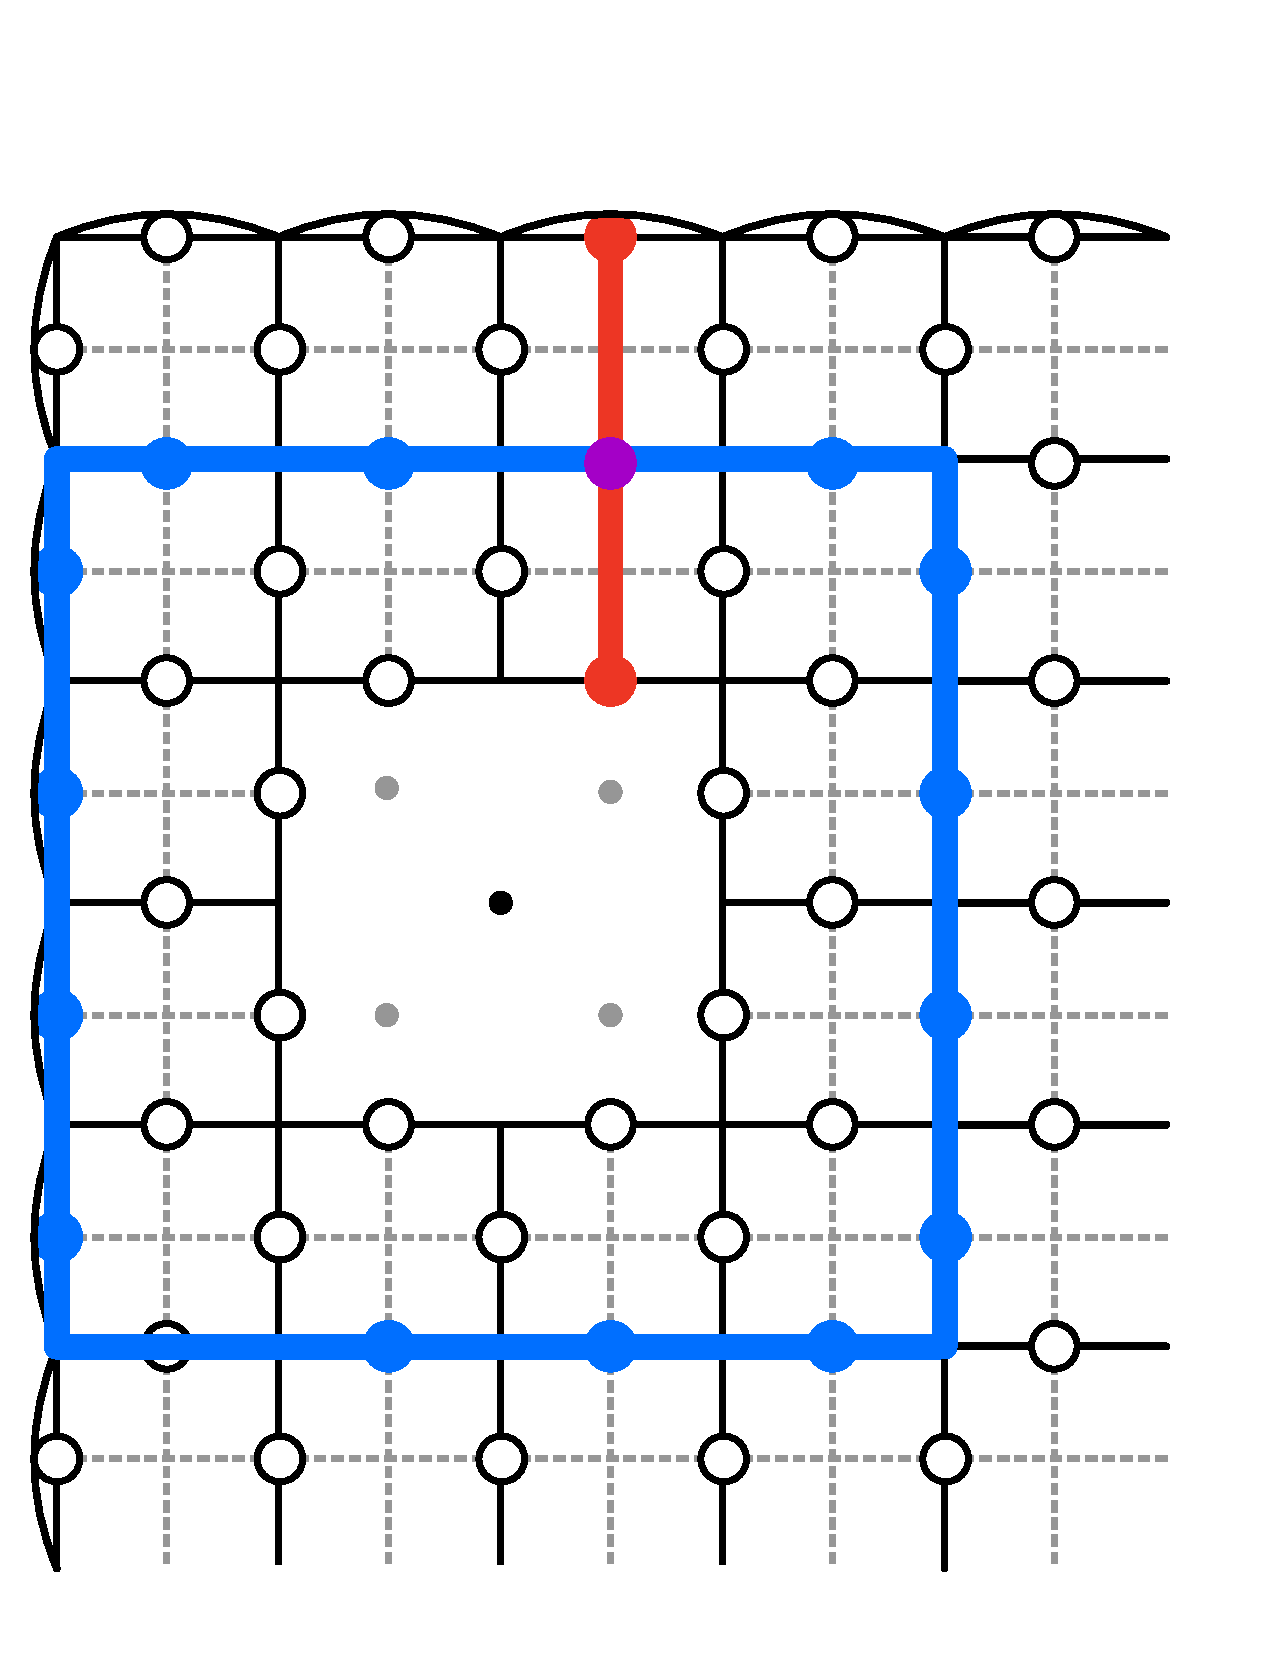
\includegraphics[width=\textwidth]{vertpunct.pdf}
             \caption{When a vertex is removed, a smooth boundary is created in the interior of the lattice. New logical operators may be constructed; one as a closed loop of $\sigma^z$ operators enclosing the puncture, and one as a string of $\sigma^x$ operators connecting the boundary of the puncture to another smooth boundary.}
             \label{fig:vertex puncture}
         \end{subfigure}
            \caption{Punctures in the toric code lattice.}
            \label{fig:punct}
    \end{figure}
    
\subsubsection{Punctures}
As previously mentioned, toric cods without boundaries yield somewhat uninteresting logical operators. More exotic logical operators can be constructed by creating defects on the lattice, such as punctures, which increase the number of encoded logical qubits without compromising the topological integrity of the system \cite{brown2017}. A puncture in the toric code is created by removing a stabilizer in a specific region of the lattice’s interior. Each puncture adds two logical qubits, since each removed stabilizer reduces the stabilizer group’s rank by two without affecting the total number of physical qubits.\newline

When a stabilizer is removed, closed $1$-chains of $\sigma^x$ or $\sigma^z$ operators enclosing the puncture can be constructed. For instance, if we remove a vertex stabilizer in the interior of the lattice, we can define a new $Z$-type logical operator as a closed loop of $\sigma^z$ operators encircling the puncture (Figure~\ref{fig:vertex puncture}). This loop represents a logical operator, as it preserves the commutation relations with the stabilizers and cannot be contracted to a point within the code. Furthermore, a new $X$-type logical operator can be realized by a string of $\sigma^x$ operators connecting the puncture’s boundary to a rough boundary, or to another puncture. This is especially remarkable because it preserves the original logical qubits $\overline{X}_{1,2}$ and $\overline{Z}_{1,2}$ defined in Section $2.5$. We can also see in Figure~\ref{fig:punct} that the newly constructed logical operators intersect once, and therefore anti-commute as expected. \newline

Punctures offer a flexible way to add encoded qubits without significantly changing the structure of the code or requiring new physical qubits. By choosing where and how many stabilizers to remove, one can customize the number of logical qubits encoded in the lattice. This adaptability, along with the topological protection afforded by the non-contractible nature of logical operators around punctures, makes them a powerful feature in surface code-based quantum error correction.\newpage

\section{Two-Dimensional Color Codes}
\subsection{Defining the Color Code}
The color code and toric code can be mainly distinguished by their different lattice structures and stabilizer structures. While the toric code is defined by placing qubits on edges, the color code places qubits on vertices and imposes two further conditions on the underlying lattice $\Lambda$:
\begin{itemize}
    \item \textbf{Valence}: Each vertex in $\Lambda$ is $3$-valent, meaning that it connects exactly three edges
    \item \textbf{Colorability}: The plaquettes of $\Lambda$ are three-colorable, meaning they can be colored with three distinct colors ($R$, $G$, and $B$) such that adjacent plaquettes have different colors
\end{itemize}
Moving forward, $\Pi$, $Q$, and $\Sigma$ will denote the sets of plaquettes, vertices, and edges in $\Lambda$. This notation is adopted in order to establish a clear distinction between the toric code and color code's differing lattice structures. Furthermore, we aim to simply future notation by defining:
    \begin{align}
        \{\mathcal{Q}(p)\}_{p\in\Pi} := \{v\in Q|v\in\partial_1e\enspace\text{for}\enspace e\in\partial_2p\}
    \end{align}
So $\mathcal{Q}(p)$ denotes the set of qubits (or vertices) that surround plaquette $p\in\Pi$. One can immediately see that each edge is adjacent to two plaquettes, and therefore is assigned two colors (corresponding to the colors of the adjacent plaquettes).\newline

The toric code associates $X$-type stabilizers to vertices and $Z$-type stabilizers to faces. In contrast, the two-dimensional color code assigns both $X$ and $Z$ stabilizers to each plaquette, acting on qubits located on the vertices of the plaquette. For $p\in P$, the stabilizer generators of the color code can be formally defined:
    \begin{align}
        \{X_p\}_{p\in\Pi} = \prod_{v\in\mathcal{Q}(p)}\sigma^x_v,\enspace\enspace\enspace \{Z_p\}_{p\in\Pi} = \prod_{v\in\mathcal{Q}(p)}\sigma^z_v.
    \end{align}
Once again, we have elected to adopt notation that is distinct from the toric code. We prove that the $X_p$ and $Z_{p'}$ commute for every $p,p'\in\Pi$ by considering two possible cases:
    \begin{enumerate}
        \item If $\mathcal{Q}(p)\cap\mathcal{Q}(p') = \emptyset$ (i.e. $X_p$ and $Z_{p'}$ do not overlap), then they trivially commute
        \item If $\mathcal{Q}(p)\cap\mathcal{Q}(p') \neq \emptyset$, by the $3$-valence of of vertices, $X_p$ and $Z_{p'}$ must share an edge. However, by the $3$-colorability of plaquettes, they cannot share consecutive edges, thus their intersection contains an even number of vertices. Formally:
            \begin{align}
                |\mathcal{Q}(p)\cap\mathcal{Q}(p')| \equiv 0\enspace\text{mod}(2).
            \end{align}
        Therefore the anti-commutativity of the respective $\sigma^x$ and $\sigma^z$ matrices cancels out.
    \end{enumerate}

Moving forward, $CC(\Lambda)$ will denote the stabilizer group of the color code defined on the lattice $\Lambda$, and $TC(\Lambda)$ will denote the stabilizer group of the toric code. All plaquettes on $\Lambda$ must have an even number of vertices, so we establish a convention where the edges of a plaquette are labeled $\{v_i\}_{i\in\{1,...,2n\}}$ for $n\in\NN$ and edges $v_i$, $v_{i+1}$ are adjacent. It is important to note that when an $X_p$ stabilizer operator acts on a plaquette, each adjacent plaquette has two $\sigma^x$ operators acting on adjacent vertices $v_i$,$v_{i+1}$ for $i\in\{1,...,2n\}$. The exact same reasoning applies to $Z_p$ operators.\newline
    \begin{figure}[h]
        \centering
        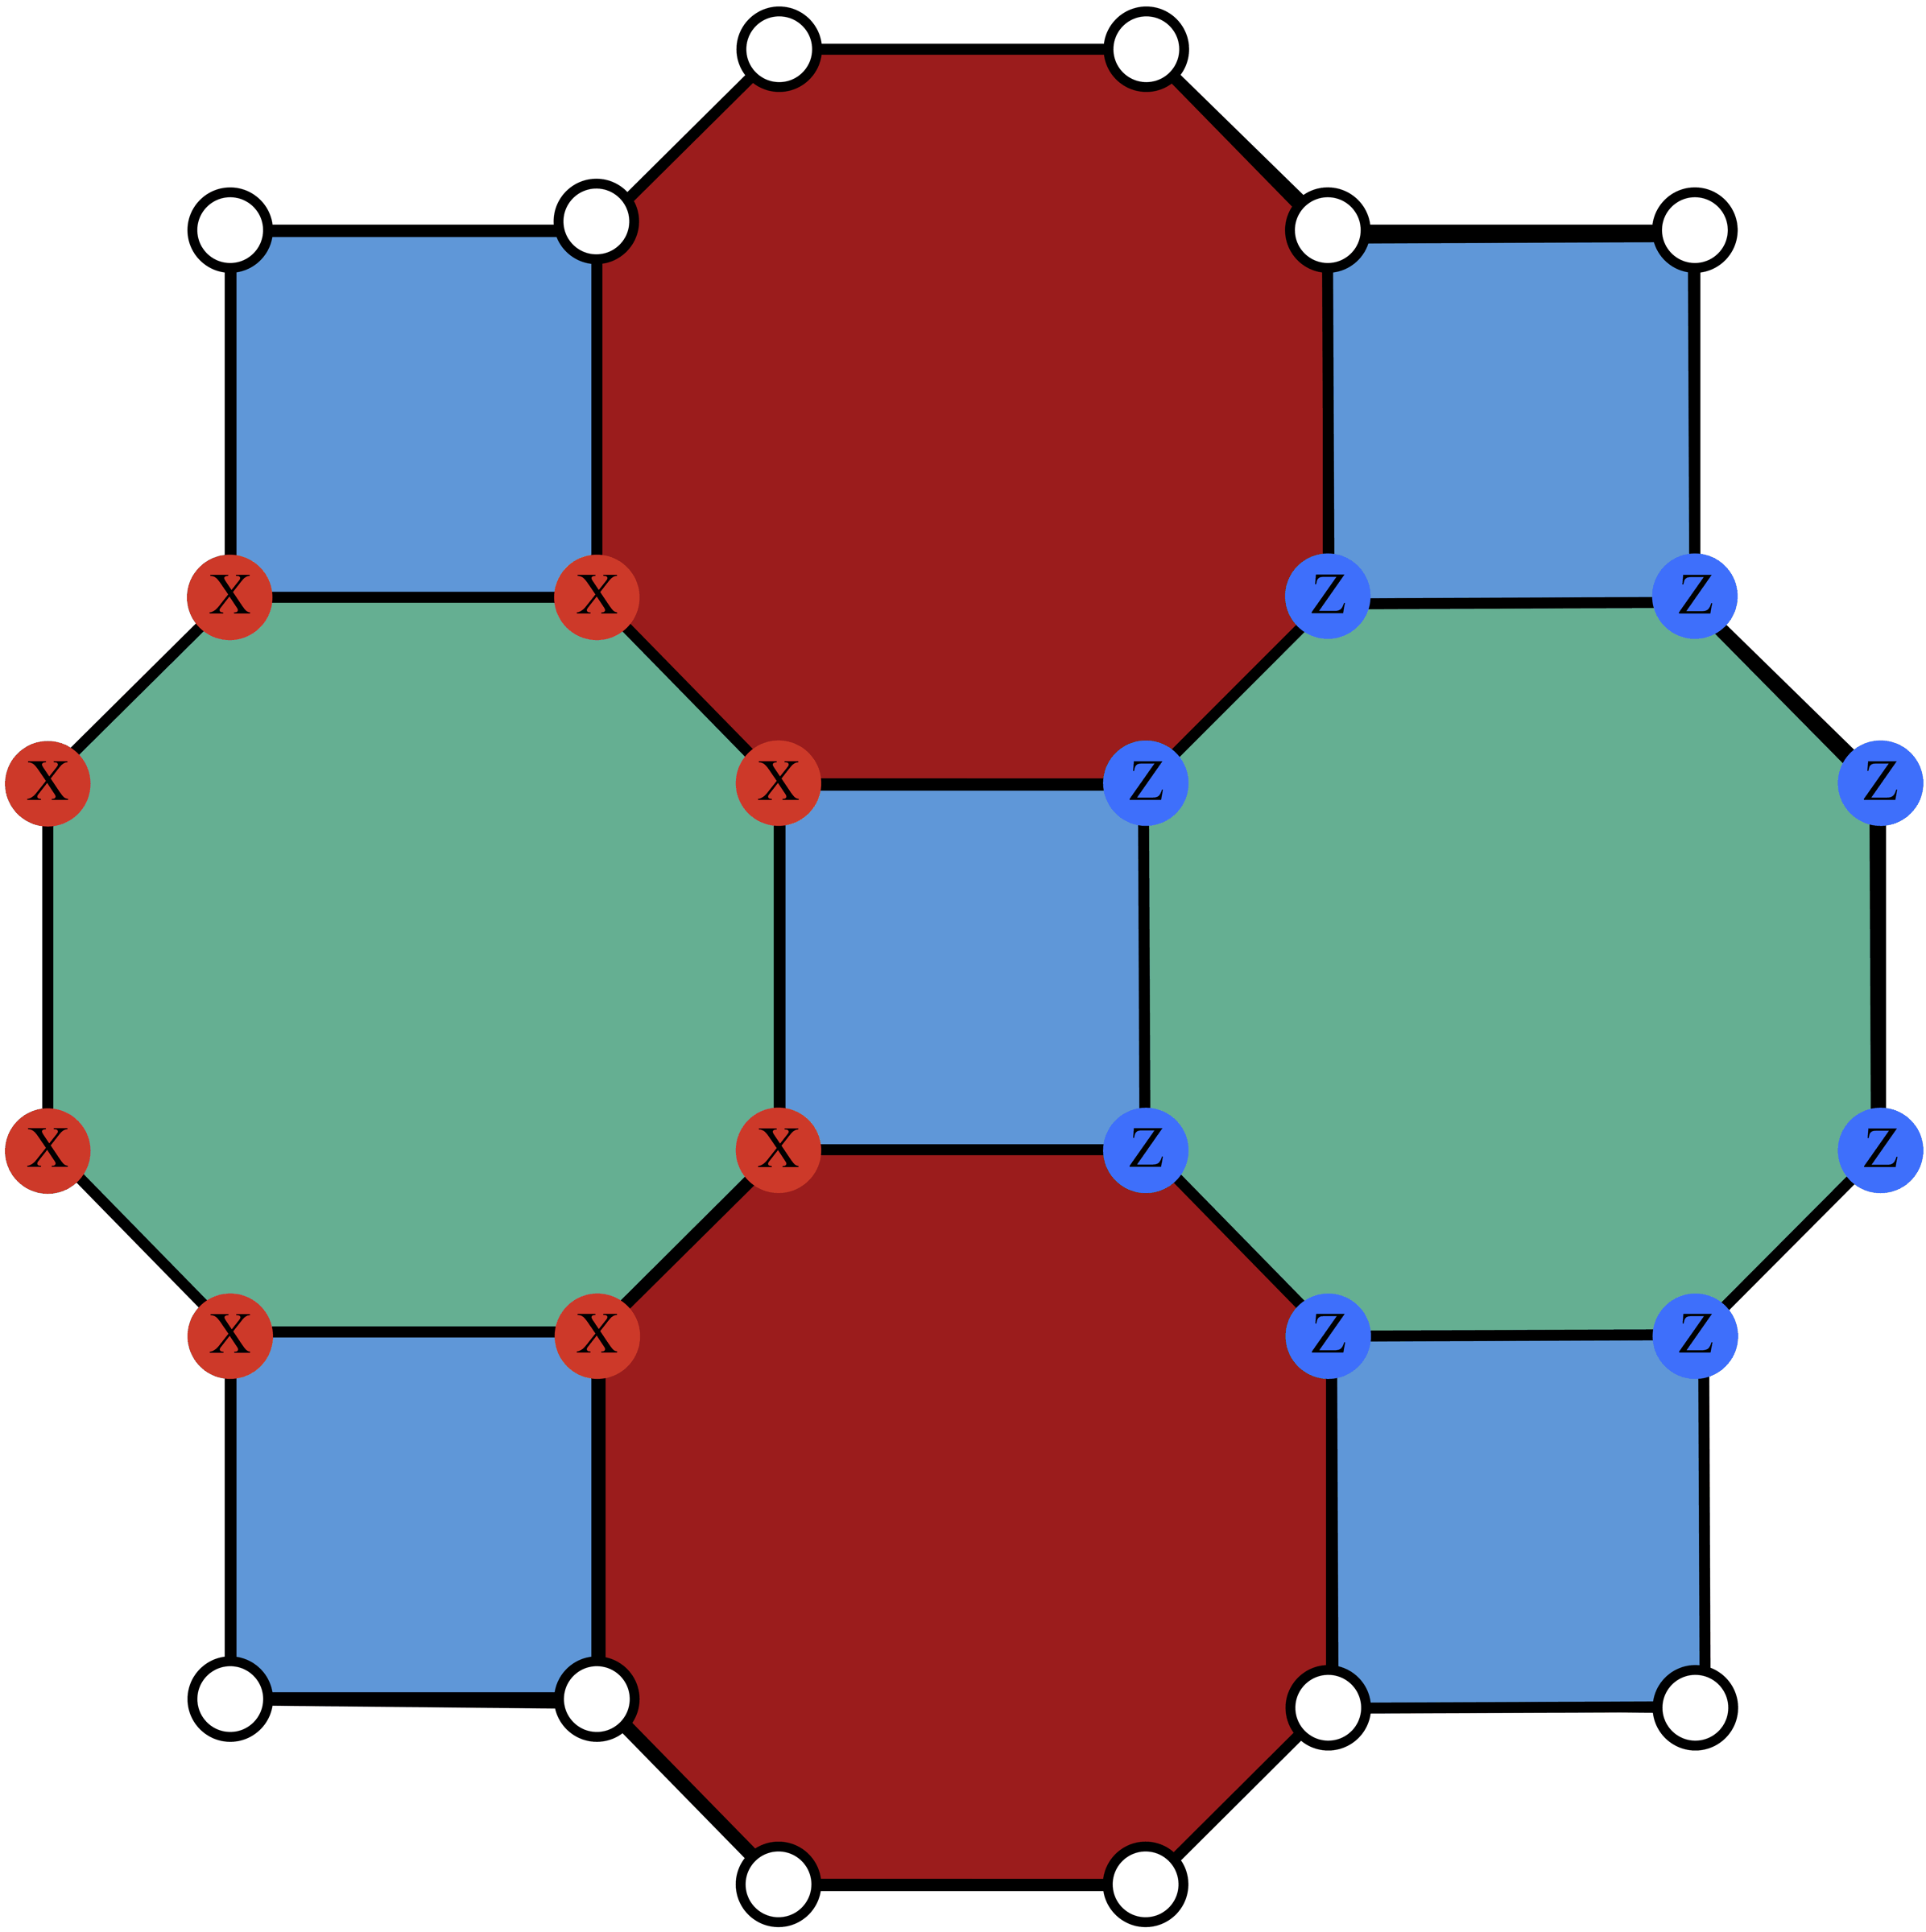
\includegraphics[width=0.4\textwidth]{color.png}
        \caption{An example of a color code defined on a two-dimensional honeycomb lattice. Each vertex is three-valent, and each plaquette is three-colorable. $X_p$ stabilizer operators apply $\sigma^x$ operators (red) to all vertices surrounding a plaquette, and $Z_p$ stabilizer operators apply $\sigma^z$ operators (blue) to all vertices surrounding a plaquette. Notice how each vertex is adjacent to a plaquette of each color.}
        \label{fig:x color code lattice}
    \end{figure}

The overall Hilbert space of the color code is $\mathcal{H}^{\otimes |Q|}_2$, where $|Q|$ denotes the total number of qubits in the system. The general state of the system is therefore described by:
    \begin{align}
        |\psi_{CC}\rangle :=\bigotimes_{v\in Q}|c_v\rangle,\enspace\enspace |c_v\rangle\in \{|0\rangle,|1\rangle\}
    \end{align}

The Hamiltonian of the system $H_{CC}$ is, unsurprisingly, given by:
    \begin{align}
        H_{CC} = -\sum_{p\in\Pi}X_p-\sum_{p\in\Pi}Z_p,
    \end{align}
and the ground states of $H_{CC}$ are the configurations that are simultaneous $+1$ eigenstates of all stabilizer operators on $\Lambda$ \cite{kubica2015}.

\subsection{Anyonic Excitations}
Anyonic excitations on the two-dimensional color code are characterized by string operators \cite{yoshida2015}. Let $\{\gamma_{\kappa_1\kappa_2}\}_{\kappa_1\kappa_2\in\{RG,RB,GB\}}$ be a $1$-chain on $\Lambda$ such that for all $e\in\gamma_{\kappa_1\kappa_2}$, $e$ has color $\kappa_1\kappa_2$. We define string operators of color $\kappa_1\kappa_2$ as follows:
    \begin{align}
        \overline{X^{\kappa_1\kappa_2}}(\gamma_{\kappa_1\kappa_2}) = \prod_{e\in\gamma_{\kappa_1\kappa_2}}\sigma^x_{v|v\in\partial_1e},\enspace\enspace\enspace\overline{Z^{\kappa_1\kappa_2}}(\gamma_{\kappa_1\kappa_2}) = \prod_{e\in\gamma_{\kappa_1\kappa_2}}\sigma^z_{v|v\in\partial_1e}.
    \end{align}
These operators commute with the stabilizers everywhere except at their endpoints $\partial_1\gamma_{\kappa_1\kappa_2}$, where they create excitations. $\overline{X^{\kappa_1\kappa_2}}(\gamma_{\kappa_1\kappa_2})$ creates magnetic vortices of color $\kappa_3\in\{R,G,B\}\setminus\{\kappa_1,\kappa_2\}$, $m_{\kappa_3}$, and $\overline{Z^{\kappa_1\kappa_2}}(\gamma_{\kappa_1\kappa_2})$ creates electric charges of color $\kappa_3\in\{R,G,B\}\setminus\{\kappa_1,\kappa_2\}$, $e_{\kappa_3}$.\newline

The quasiparticle excitations obey the following fusion rules:
    \begin{align}
        m_R\times m_G\times m_B = 1,\enspace\enspace\enspace e_R\times e_G\times e_B = 1.
    \end{align}
Furthermore, $e$ and $m$ quasiparticles of the same color exhibit trivial braiding statistics. Conversely, $e $ and $m$ quasiparticles of different colors exhibit non-trivial braiding statistics. These braiding statistics can be more rigorously understood by constructing an isomorphism between the excitations of of color code and the excitations of the toric code. However, before this can be done, the equivalence of the two codes must be discussed in detail.

\subsection{Equivalence Theorem in Two Dimensions}
It is a well known result that the two-dimensional color code on a closed manifold is equivalent to two copies of the toric code. The most cited proof of this equivalence was presented by Aleksander Kubica, Beni Yoshida, and Fernando Pastawsk, and the proof presented here is largely based on their work \cite{kubica2015}.\newline

The equivalence between the color code and toric code can is formalized by a local unitary Clifford transformation $U$ that relates the respective lattices through conjugation. Before stating the theorem of existence of $U$, it is important to describe the concept of \emph{shrunk lattices}. The shrunk lattice $\{\Lambda_i\}_{i\in\{R,G,B\}}$ is obtained by shrinking plaquettes of color $i$; for example the structure of $\Lambda_R$ consists of:
    \begin{itemize}
        \item \textbf{Vertices}: centers of plaquettes in $\Lambda$ of color $R$
        \item \textbf{Edges}: edges of $\Lambda$ of color $GB$
        \item \textbf{Plaquettes}: plaquettes in $\Lambda$ of colors $G$ and $B$
    \end{itemize}
    \begin{theorem}
    Let $CC(\Lambda)$ be a two-dimensional color code on a lattice $\Lambda$ without boundaries colored with $R$, $G$ and $B$. There exists a local unitary Clifford transformation $U$, such that:
        \begin{align}
            U[CC(\Lambda)]U^\dagger = TC(\Lambda_R)\otimes TC(\Lambda_G),
        \end{align}
    where $TC(\Lambda_R)$ and $TC(\Lambda_G)$ are two independent toric codes on the shrunk lattices $\Lambda_R$ and $\Lambda_G$. Furthermore, one can write:
        \begin{align}
            U = \bigotimes_{p\in\Pi_B}U_p,
        \end{align}
    where $\Pi_B$ represents the set of plaquettes of color $B$, and $U_p$ is a unitary Clifford transformation acting on the qubits $\mathcal{Q}(p)$.
    \end{theorem}

The transformation $U$ - commonly referred to as the \emph{disentangling transformation} - acts locally on faces of color $B$ in $\Lambda$ and maps the stabilizers of $CC(\Lambda)$ to those of two decoupled copies of the toric code $TC(\Lambda_R)$ and $TC(\Lambda_G)$. This results in two distinct stabilizer groups on the shrunk lattices, effectively separating the color code into two copies of the toric code.\newline

Before proving Theorem $3.1$, we consider the desired action of $\{U\}_{p\in\Pi}$ from a practical perspective. In principle, the disentangling operator maps $\sigma^z$ and $\sigma^x$ operators from vertices to edges, as the toric code places such operators on edges rather than vertices. There are four configurations to consider:
    \begin{align}
        \{\sigma^z_{v_i}\sigma^z_{v_{i+1}}\}_{i\in\{1,...,2n-1\}}&\xrightarrow{U_p}\sigma^z_{e|\partial_1e := \{v_i,v_{i+1}\}}\\\{\sigma^x_{v_i}\sigma^x_{v_{i+1}}\}_{i\in\{1,...,2n-2\}}&\xrightarrow{U_p}\sigma^x_{e|\partial_1e := \{v_{i-1},v_i\}}\sigma^x_{e|\partial_1e := \{v_{i+1},v_{i+2}\}}\\
        X_p\sigma^z_{v_{2n}}\sigma^z_{v_1}&\xrightarrow{U_p}\sigma^z_{e|\partial_1e := \{v_{2n},v_1\}}\\
        X_p\sigma^x_{v_i}\sigma^x_{v_{i+1}}&\xrightarrow{U_p}\sigma^x_{e|\partial_1e := \{v_{i-1},v_i\}}\sigma^x_{e'|\partial_1e' := \{v_{i+1},v_{i+2}\}}
    \end{align}
These transformations are perhaps beset understood through their graphical representations in Figure~\ref{fig:x transformation} Theorem $1.1$ claims that the transformation $U_p$ exists for all $p\in\Pi$.\newline
        \begin{figure}[h]
            \centering
            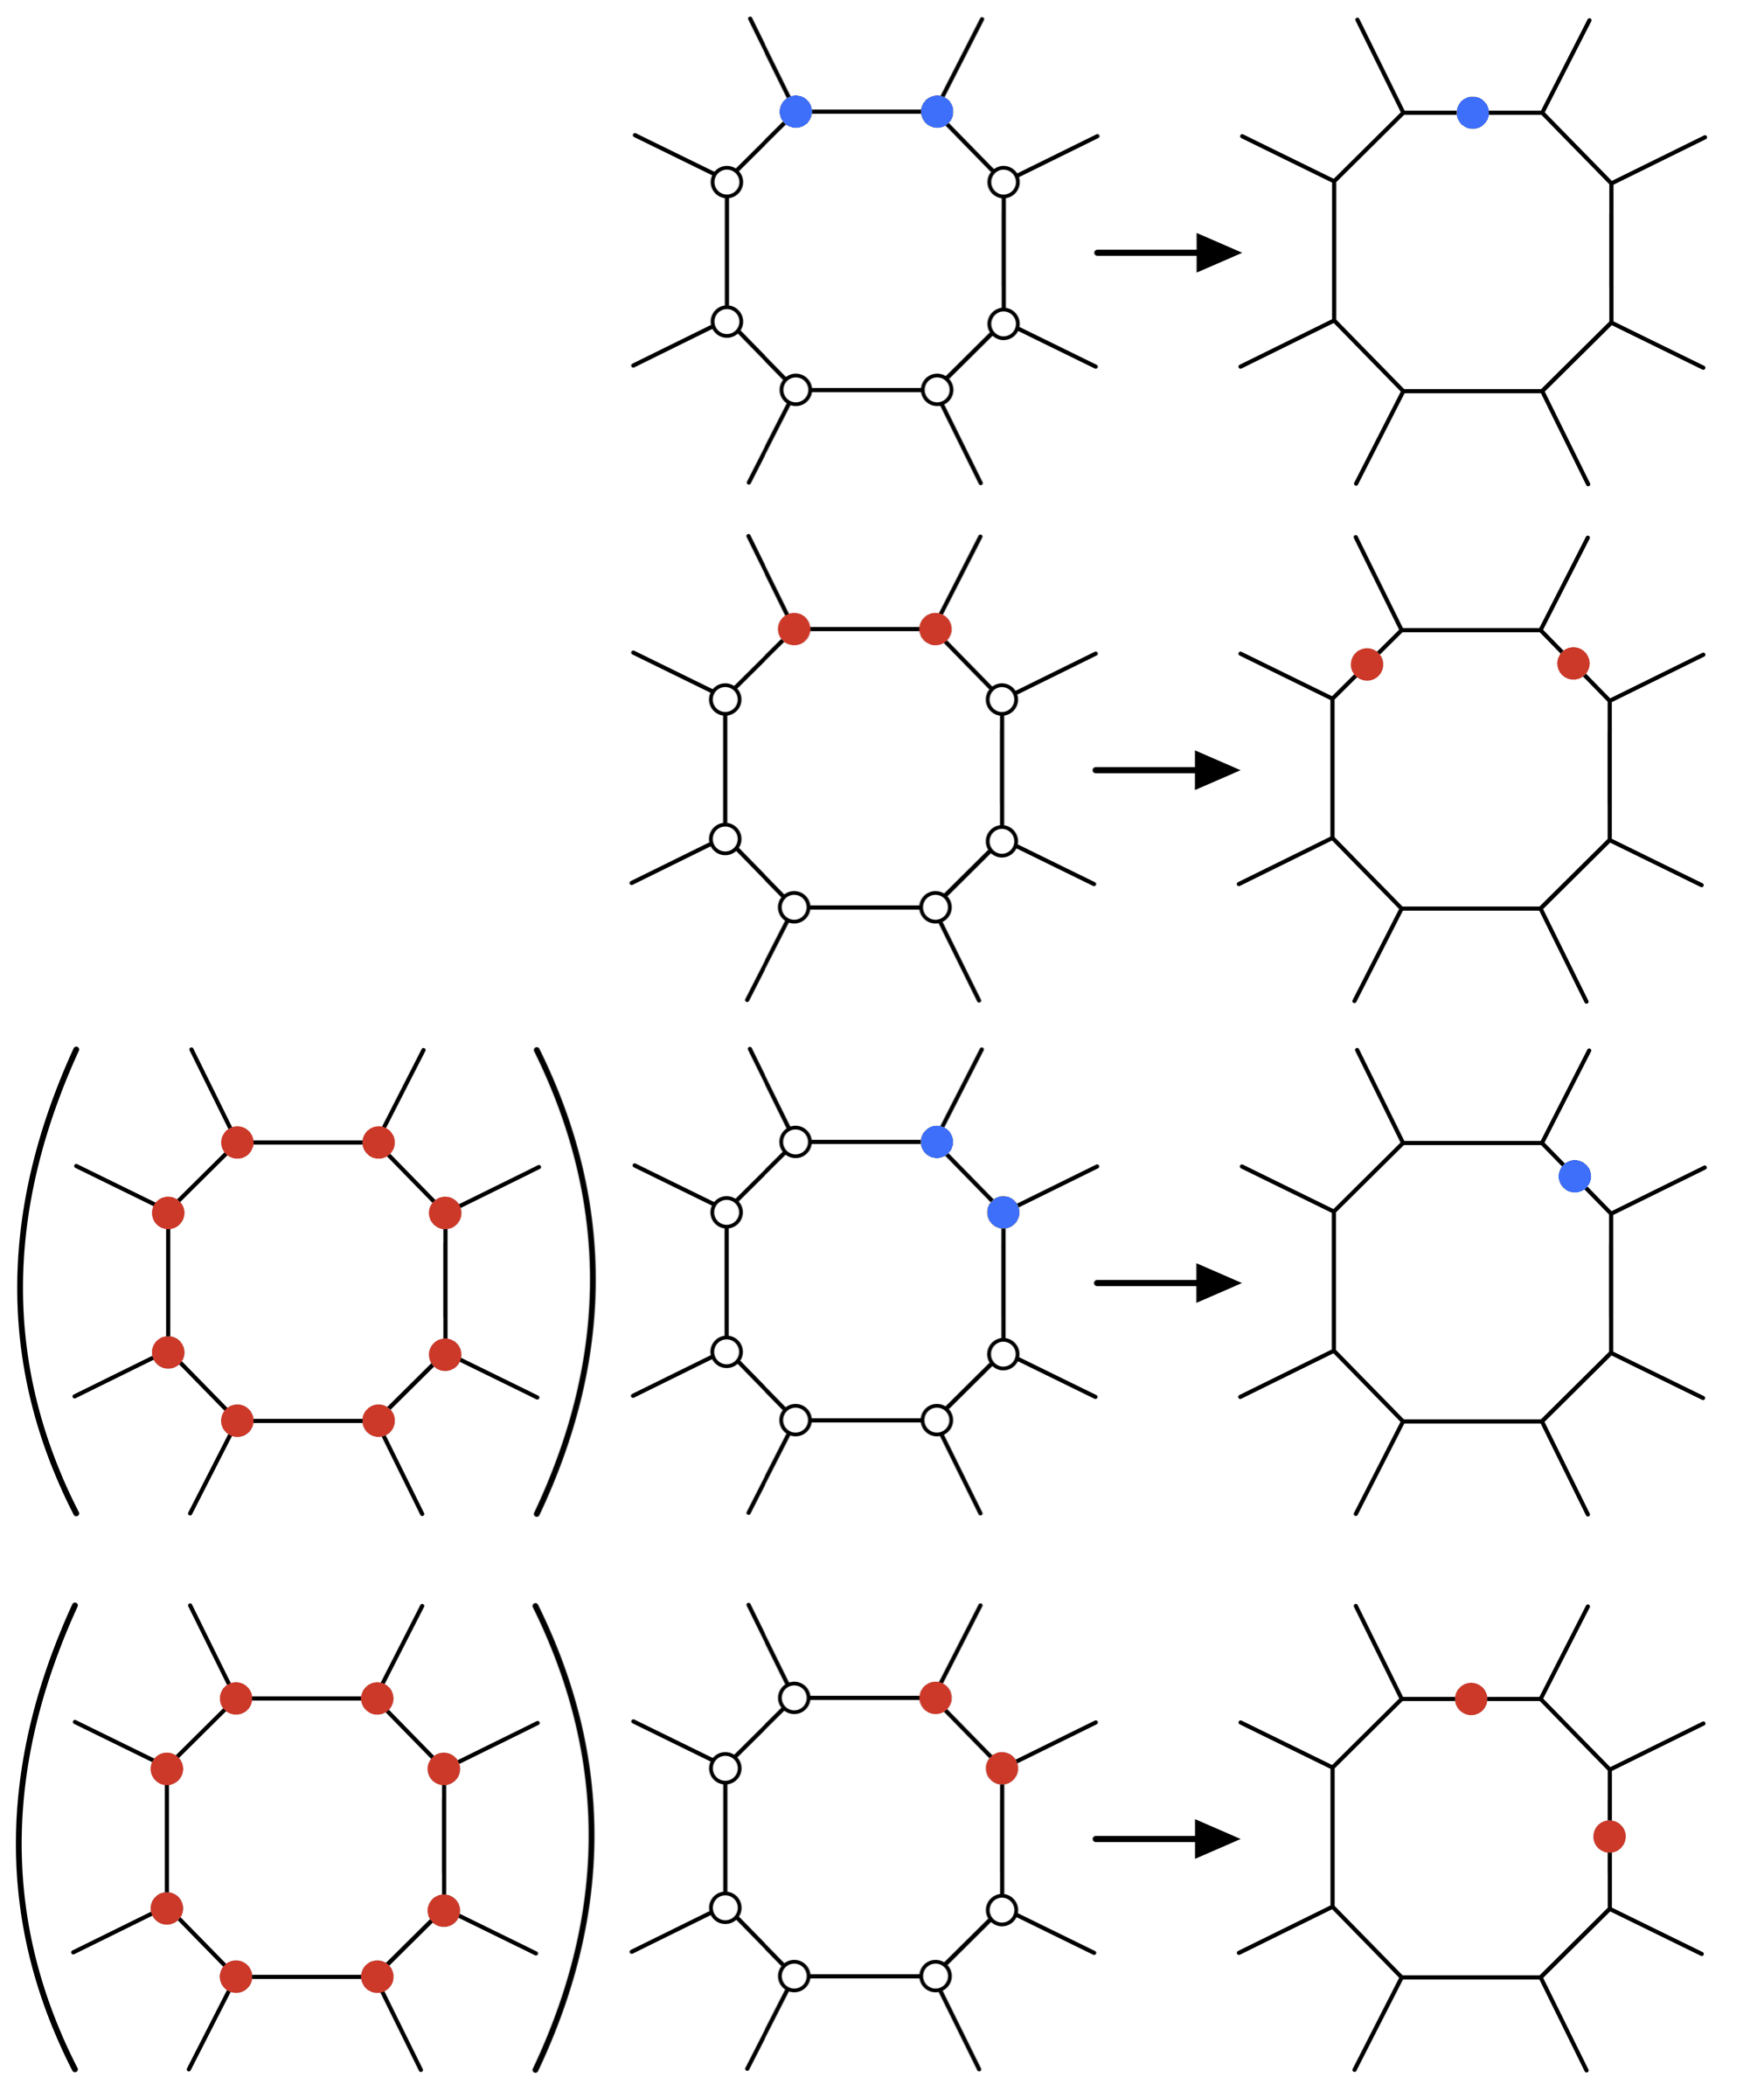
\includegraphics[width=0.4\textwidth]{Trans.png}
            \caption{Graphical representation of the transformations we desire from the disentangling operator. As usual, $\sigma^x$ operators are in red and $\sigma^z$ operators are in blue.}
            \label{fig:x transformation}
        \end{figure}

Let us study how $Z_p$ and $X_p$ stabilizers transform according to equations $(104) - (107)$. We consider how the stabilizer $Z_p$ is transformed for each possible color of $p$.
    \begin{itemize}
        \item For $p\in\Pi_R$, $U_p$ maps the $\sigma^z$ operators in $Z_p$ from each vertex to the edges of color $RB$
        \item For $p\in\Pi_G$, $U_p$ maps the $\sigma^z$ operators in $Z_p$ to the edges of color $GB$
        \item For $p\in\Pi_B$, $U_p$ maps the $\sigma^z$ operators in $Z_p$ to the edges of color $RB$
    \end{itemize}

Meanwhile, $U_p$ maps the $\sigma^x$ operators in $X_p$ to the edges adjacent to $p$. Formally:
    \begin{align}
        \{X_p\}_{p\in\Pi}\xrightarrow{U_p}\prod_{e\notin\partial_2p|\partial_1e\cup\partial_1e'\neq 0\;\text{for}\;e'\in\partial_2p}\sigma^x_e
    \end{align}
    \begin{figure}[h]
         \centering
         \begin{subfigure}[b]{0.4\textwidth}
             \centering
             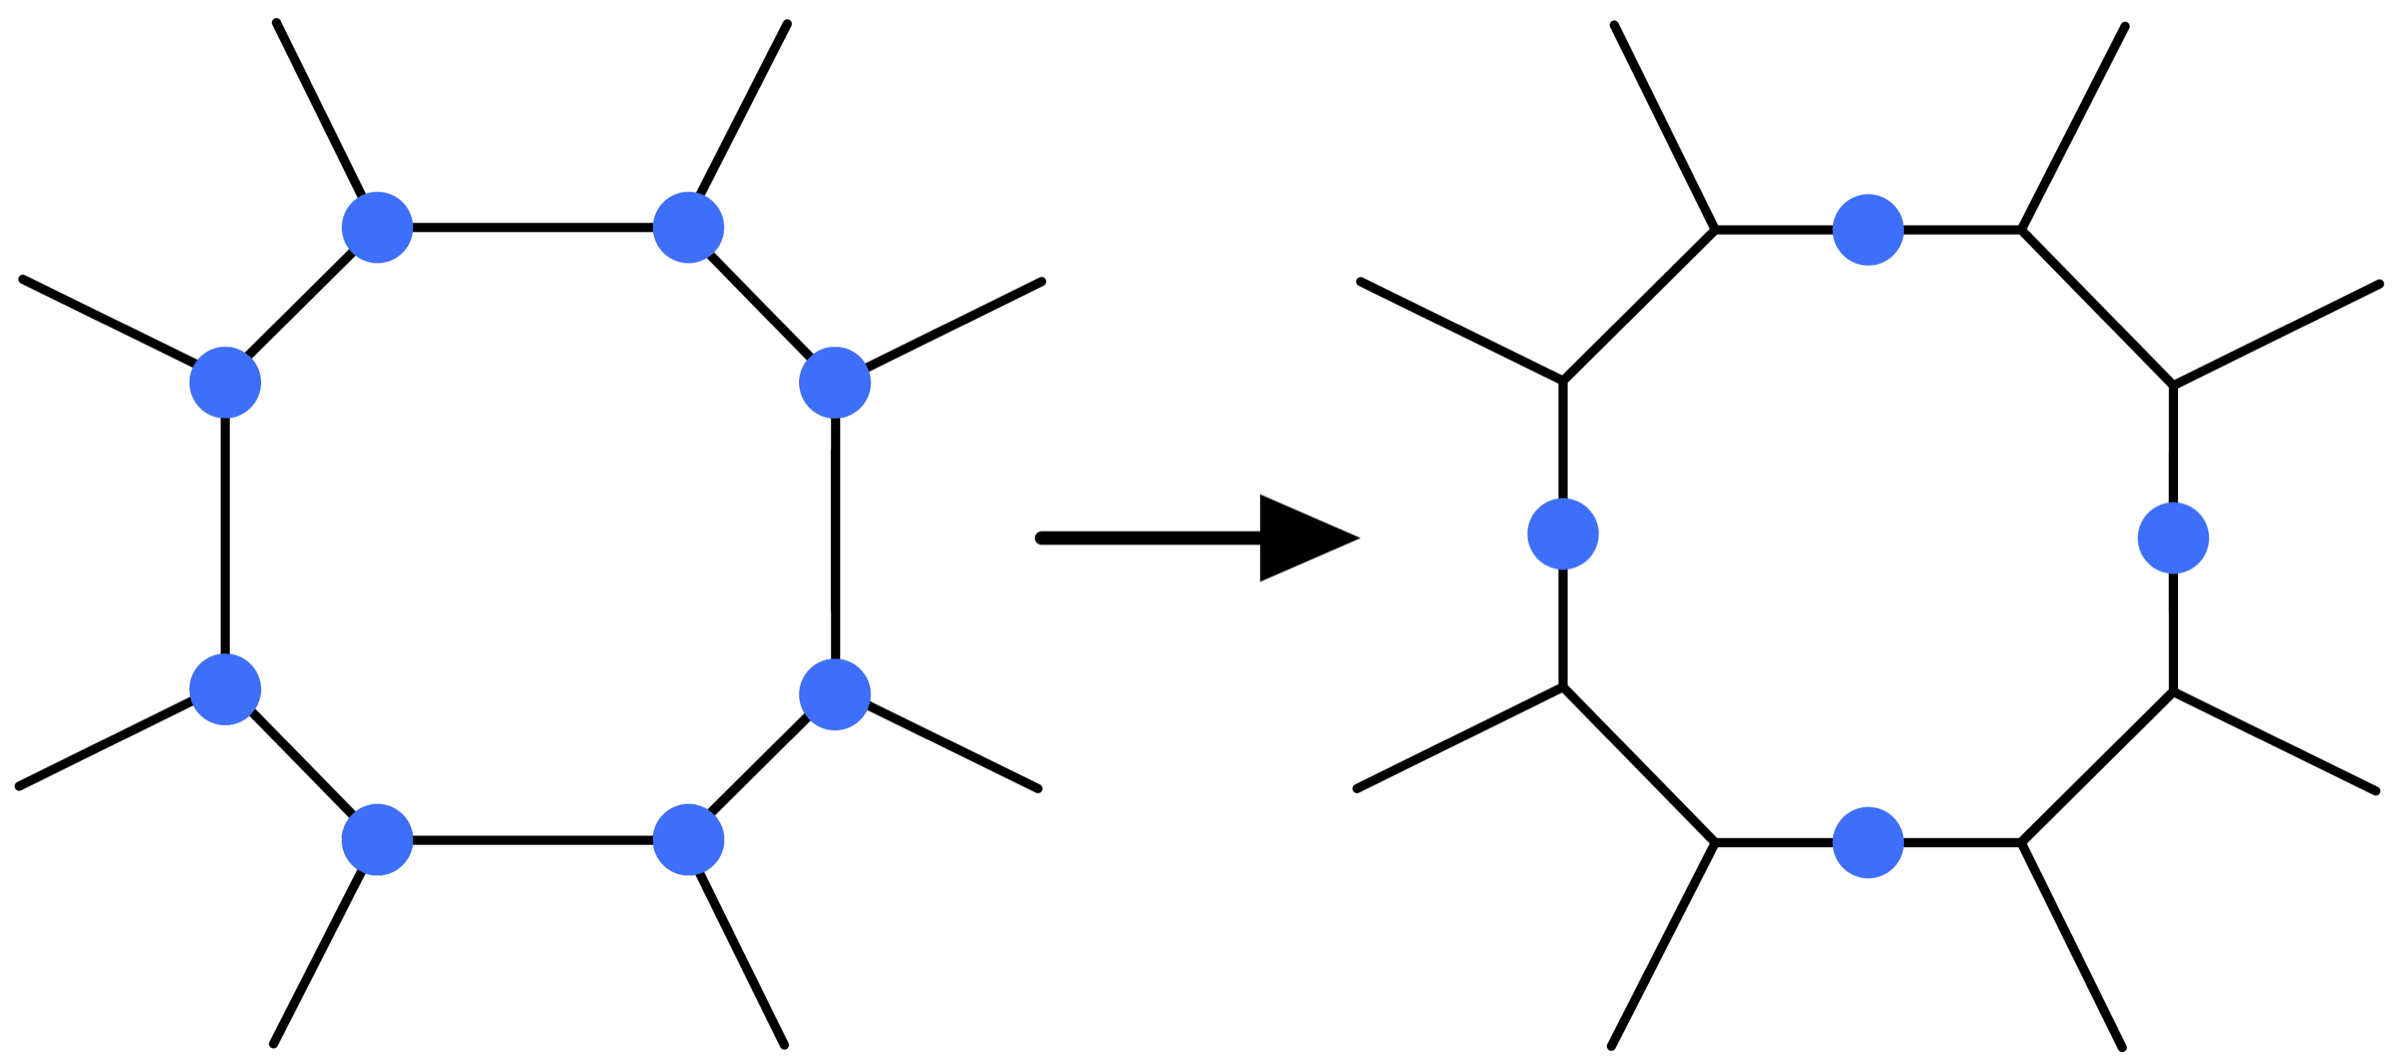
\includegraphics[width=\textwidth]{stab_trans1.png}
             \caption{Transformation $U_pZ_pU^\dagger_p$.}
             \label{fig:x stab trans}
         \end{subfigure}
         \enspace\enspace\enspace
         \begin{subfigure}[b]{0.4\textwidth}
             \centering
             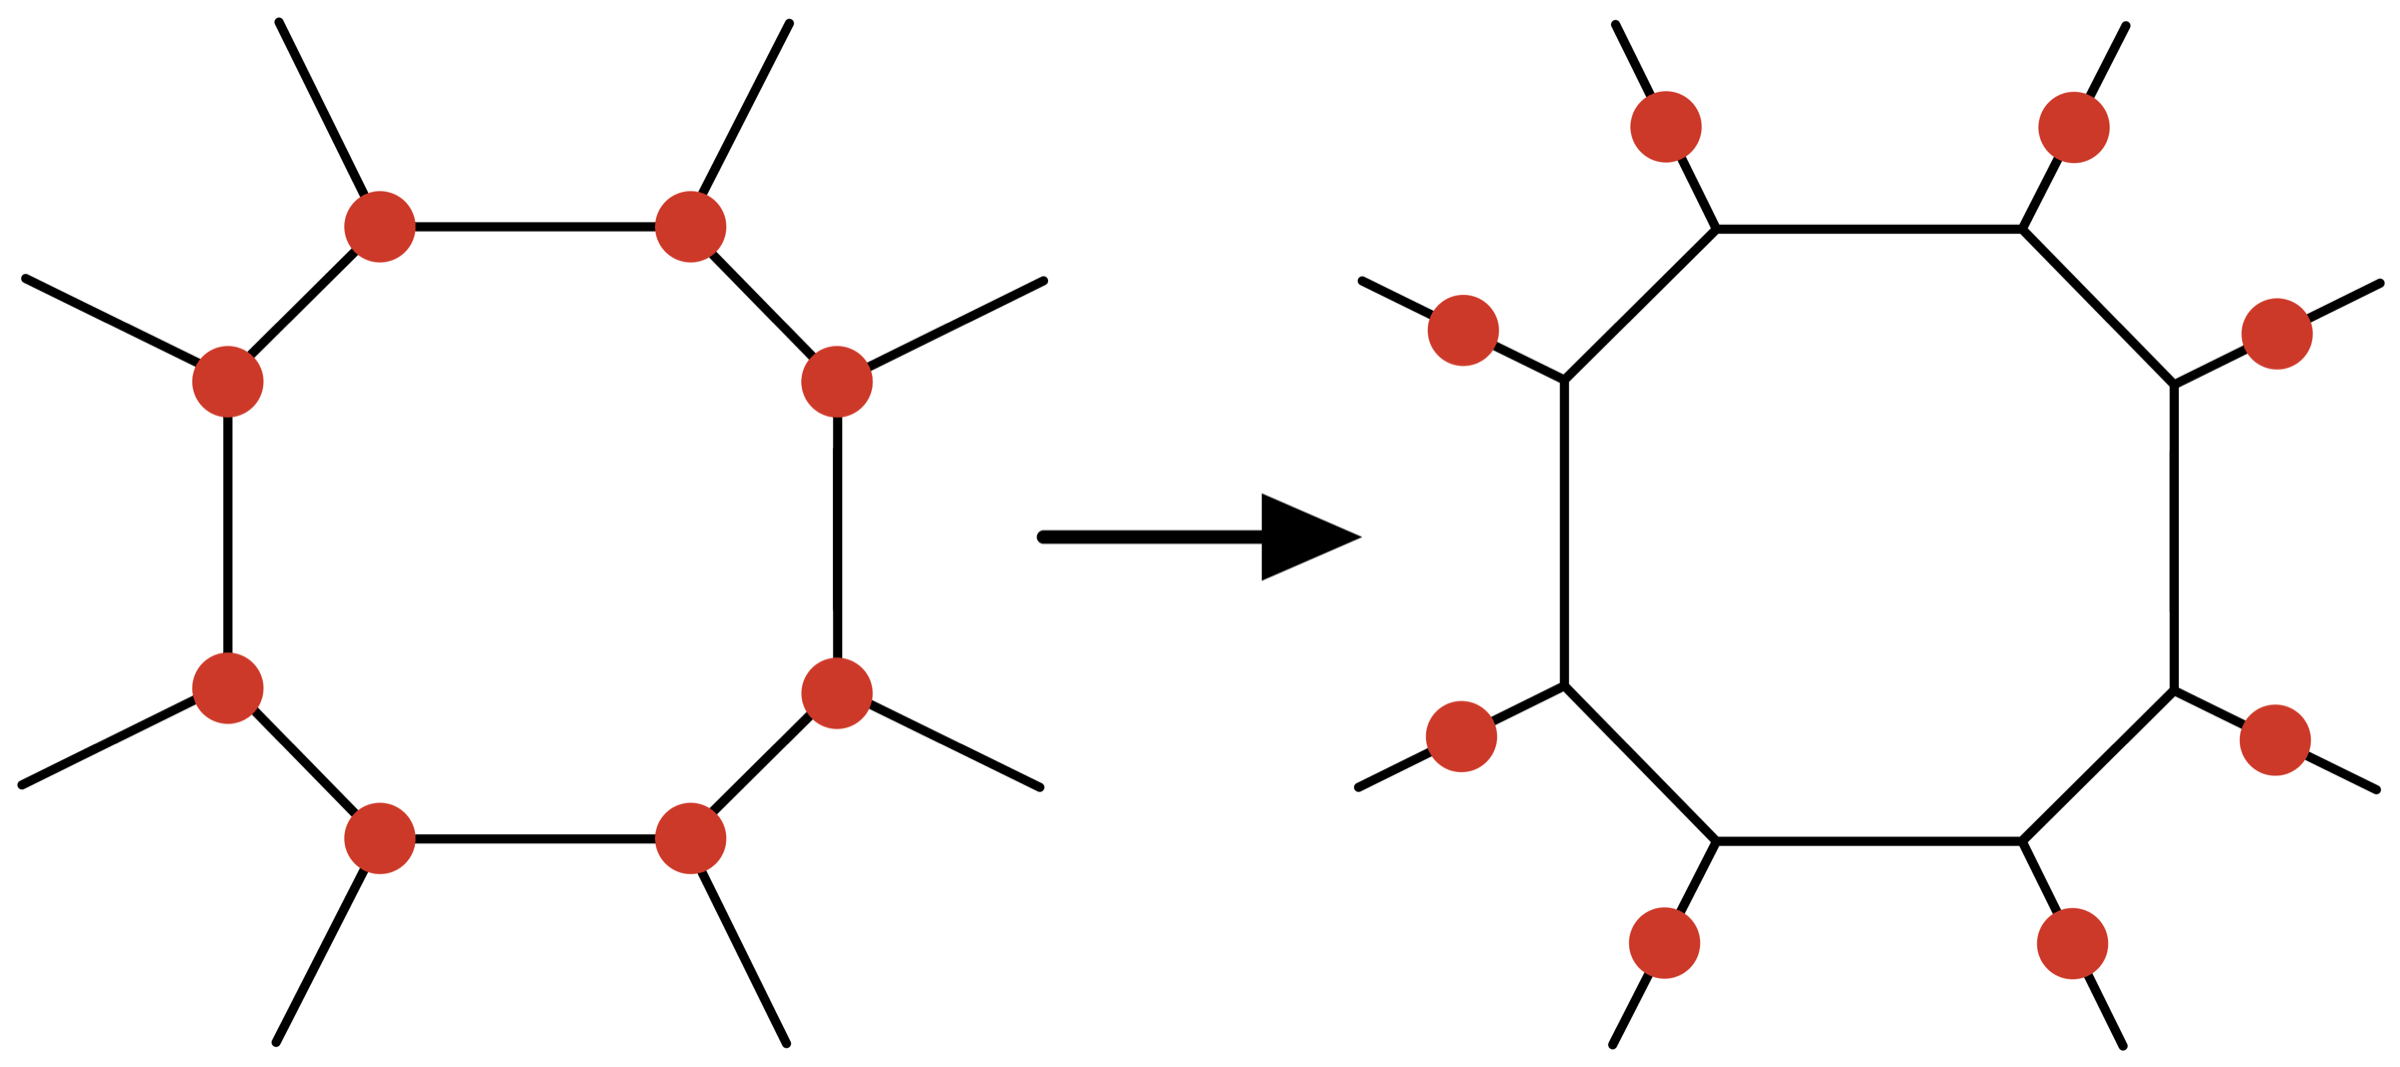
\includegraphics[width=\textwidth]{stab_trans2.png}
             \caption{Transformation $U_pX_pU^\dagger_p$.}
             \label{fig:z stab trans}
         \end{subfigure}
            \caption{Transformation of stabilizer operators under the desired action of $U_p$.}
            \label{fig:stab trans}
    \end{figure}
We now wish to rigorously prove the existence of $U  = \bigotimes_{p\in\Pi_B}U_p$, which requires the development of some formalism concerning Pauli subgroups. Moving forward, \textbf{Pauli}$(n)$ will denote the Pauli group on $n$ qubits.
    \begin{definition}(Isomorphic Pauli Subgroups). 
        \emph{For $\mathcal{P}_1,\mathcal{P}_2\in\textbf{Pauli}(n)$, we say that $\mathcal{P}_1$ and $\mathcal{P}_2$ are isomorphic if and only if there exists a unitary Clifford transformation $U$ such that:}
            \begin{align}
                U\mathcal{P}_1U^\dagger = \mathcal{P}_2.
            \end{align}
    \end{definition}
    \begin{definition}(Center of a subgroup).
        \emph{Let $G$ be a group, and $H$ be a subgroup of $G$. The center of $H$ is defined:}
            \begin{align}
                Z(H) := \{z\in H|[h,z] = 0\enspace\forall\enspace h\in H\}.
            \end{align}
    \end{definition}\newpage
    \begin{lemma}
        Two Pauli subgroups $\mathcal{P}_1,\mathcal{P}_2\subset\textbf{Pauli}(n)$ are isomorphic if and only if:
            \begin{align}
                G(\mathcal{P}_1) = G(\mathcal{P}_2),\enspace\enspace\text{and}\enspace\enspace G(Z(\mathcal{P}_1)) = G(Z(\mathcal{P}_2)),
            \end{align}
        where $G(\mathcal{P})$ denotes the number of independent generators of $\mathcal{P}\subset\textbf{Pauli}(n)$.
    \end{lemma}
    
Having mentioned the notion of generators, let us explore it further. For two independent sets of generators $\{g_i\}$ and $\{h_i\}$ of isomorphic groups $G$ and $H$, respectively, we say that $\{g_i\}$ and $\{h_i\}$ have the same commutation relations if:
    \begin{align}
        g_ig_j = (-1)^{c_{i,j}}g_jg_i,\enspace\enspace\text{and}\enspace\enspace h_ih_j = (-1)^{c_{i,j}}h_jh_i\enspace\enspace\text{for}\enspace\enspace (c_{i,j} = 0,1),
    \end{align}
where the object $c_{i,j}$ is symmetric in it's indices and, trivially, $c_{i,i} = 0$. Using the tools we have developed, the following lemma may be considered:
    \begin{lemma}
        Let $\mathcal{P}_1,\mathcal{P}_2\subset\textbf{Pauli}(n)$ be isomorphic subgroups generated by $\{g_j\}$ and $\{h_j\}$, respectively. If $\{g_j\}$ and $\{h_j\}$ have the same commutation relations, then there exists a unitary Clifford transformation $U$ such that:
            \begin{align}
                Ug_jU^\dagger = h_j\enspace\forall\enspace j.
            \end{align}
    \end{lemma}
    \begin{definition}(Overlap group of the stabilizer group).
        \emph{Let $H\subseteq Q$ denote a subset of vertices. The overlap group of the stabilizer group $CC(\Lambda)$ on $H$ is defined:}
            \begin{align}
                \mathcal{O}_H = \langle u|u\in H\cap CC(\Lambda)\rangle.
            \end{align}
    \end{definition}
Essentially the overlap of $CC(\Lambda)$ on the region $H\subseteq Q$ is the group generated by the generators of $CC(\Lambda)$ in $H$.\newline

Consider a plaquette $p_B\in\Pi_B$, which must necessarily have $2n$ vertices for $n\in\NN$, and two adjacent plaquettes $p_R\in\Pi_R$ and $p_G\in\Pi_G$ (so $\partial_2p_B\cap\partial_2p_R\neq\emptyset$ and $\partial_2p_B\cap\partial_2p_G\neq\emptyset$). The overlap group of $CC(\Lambda)$ on $p_B$ is generated by:
    \begin{align}
        \mathcal{O}_{p_B} = \langle \sigma^x_{v_i}\sigma^x_{v_{i+1}},\sigma^z_{v_i}\sigma^z_{v_{i+1}}\rangle,
    \end{align}
for $i\in\{1,...,2n\}$. And the overlap of stabilizer groups of $TC(\Lambda_R)$ and $TC(\Lambda_G)$ on $p_R\cup p_G$ is generated by:
    \begin{align}
        \mathcal{O}_{p_R\cup p_G} = \langle\sigma^z_{e|\partial_1e := \{v_i,v_{i+1}\}},\sigma^x_{e'|\partial_1e' := \{v_{i-1},v_i\}}\sigma^x_{e''|\partial_1e'' := \{v_{i+1},v_{i+2}\}}\rangle,
    \end{align}
for $i\in\{1,...,2n\}$.\newpage
    \begin{claim}
        $\mathcal{O}_{p_B}$ and $\mathcal{O}_{p_R\cup p_G}$ are isomorphic.
    \end{claim}
    \begin{proof}
        We can easily count the independent generators of $\mathcal{O}_{p_B}$ and $\mathcal{O}_{p_R\cup p_G}$. For each $p\in\Pi$ with $|\mathcal{Q}(p)|=2n$ for $n\in\NN$:
            \begin{itemize}
                \item $\mathcal{O}_{p_B}$ has $2n-1$ $\sigma^x_{v_i}\sigma^x_{v_{i+1}}$ generators, and $2n-1$ $\sigma^z_{v_i}\sigma^z_{v_{i+1}}$ generators.
                \item $\mathcal{O}_{p_R\cup p_G}$ has $2n$ $\sigma^z_{e|\partial_1e := \{v_i,v_{i+1}\}}$ generators, and $2n-2$ $\sigma^x_{e'|\partial_1e' := \{v_{i-1},v_i\}}\sigma^x_{e''|\partial_1e'' := \{v_{i+1},v_{i+2}\}}$ generators.
            \end{itemize}
        We find that both overlap groups have $4n-2$ generators. Therefore:
            \begin{align}
                G(\mathcal{O}_{p_B}) = G(\mathcal{O}_{p_R\cup p_G})\\
                G(Z(\mathcal{O}_{p_B})) = G(Z(\mathcal{O}_{p_R\cup p_G})).
            \end{align}
        By Lemma $3.4$, $\mathcal{O}_{p_B}$ and $\mathcal{O}_{p_R\cup p_G}$ are isomorphic. 
    \end{proof}
    \begin{claim}
        Let $\{g_i\}$ and $\{h_i\}$ be the sets of independent generators of $\mathcal{O}_{p_B}$ and $\mathcal{O}_{p_R\cup p_G}$, respectively. $\{g_i\}$ and $\{h_i\}$ have the same commutation relations.
    \end{claim}
    \begin{proof}
        We start by expressing the generators $\{g_i\}$ and $\{h_i\}$ explicitly. We may label the $4n-2$ generators of $\mathcal{O}_{p_R\cup p_G}$ as follows:
            \begin{align}
                \{h_i\}_{i\in\{1,...,2n\}} &= \sigma^z_{e|\partial_1e := \{i,i+1\}}\\
                \{h_i\}_{i\in\{2n+1,...,4n-2\}} &= \sigma^x_{e'|\partial_1e' := \{i-1,i\}}\sigma^x_{e''|\partial_1e'' := \{i+1,i+2\}},
            \end{align}
        and label the the generators of $\mathcal{O}_{p_B}$ as:
            \begin{align}
                \{g_i\}_{i\in\{1,...,2n-1\}} &= \sigma^z_{v_i}\sigma^z_{v_{i+1}}\\
                g_{2n} &= (\prod^{2n}_{i = 1}\sigma^x_{v_i})\sigma^z_{v_{2n}}\sigma^z_{v_1}\\
                \{g_i\}_{i\in\{2n+1,...,4n-2\}} &= \sigma^x_{v_i}\sigma^x_{v_{i+1}}.
            \end{align}
        Using these explicit expressions for the generators of $\mathcal{O}_{p_B}$ and $\mathcal{O}_{p_R\cup p_G}$, one can directly check that $\{g_i\}$ and $\{h_i\}$ have the same commutation relations. 
    \end{proof}
We have proven that $\mathcal{O}_{p_B}$ and $\mathcal{O}_{p_R\cup p_G}$ are isomorphic, and that their generators have the same commutation relations. Therefore, by Lemma $3.5$, there exists a unitary Clifford transformation $U_{p_B}$ such that:
    \begin{align}
        U_{p_B}g_iU^\dagger_{p_B} = h_i\enspace\forall\enspace i\in\{1,...,4n-2\}.
    \end{align}
Thus we can construct the transformation $U = \otimes_{p\in\Pi_B}U_p$ that transforms $CC(\Lambda)$ into $TC(\Lambda_R)\otimes TC(\Lambda_G)$, proving Theorem $3.1$.

\subsection{Color Code with Boundaries}
The total boundary of a topological color code $CC(\Lambda)$ defined on a two-dimensional lattice $\Lambda$ can be expressed:
    \begin{align}
        \partial\Lambda = \bigcup^n_{i=1}\partial\Lambda^i,
    \end{align}
where each $\partial\Lambda^i$ is assigned a color. The boundary $\partial\Lambda^i$ has color $\kappa_1\in\{R,G,B\}$ if all the plaquettes adjacent to $\partial\Lambda^i$ have colors $\kappa_2$ and $\kappa_3$ for $\kappa_2,\kappa_3\in\{R,G,B\}\setminus\{\kappa_1\}$. These color codes encode $n-2\chi$ logical qubits, and admit transversal logical Hadamard gates $\overline{\mathcal{H}}$ and phase gates $\overline{R}_2$. These gates will be studied in detail in later sections.\newline
        \begin{figure}[h]
            \centering
            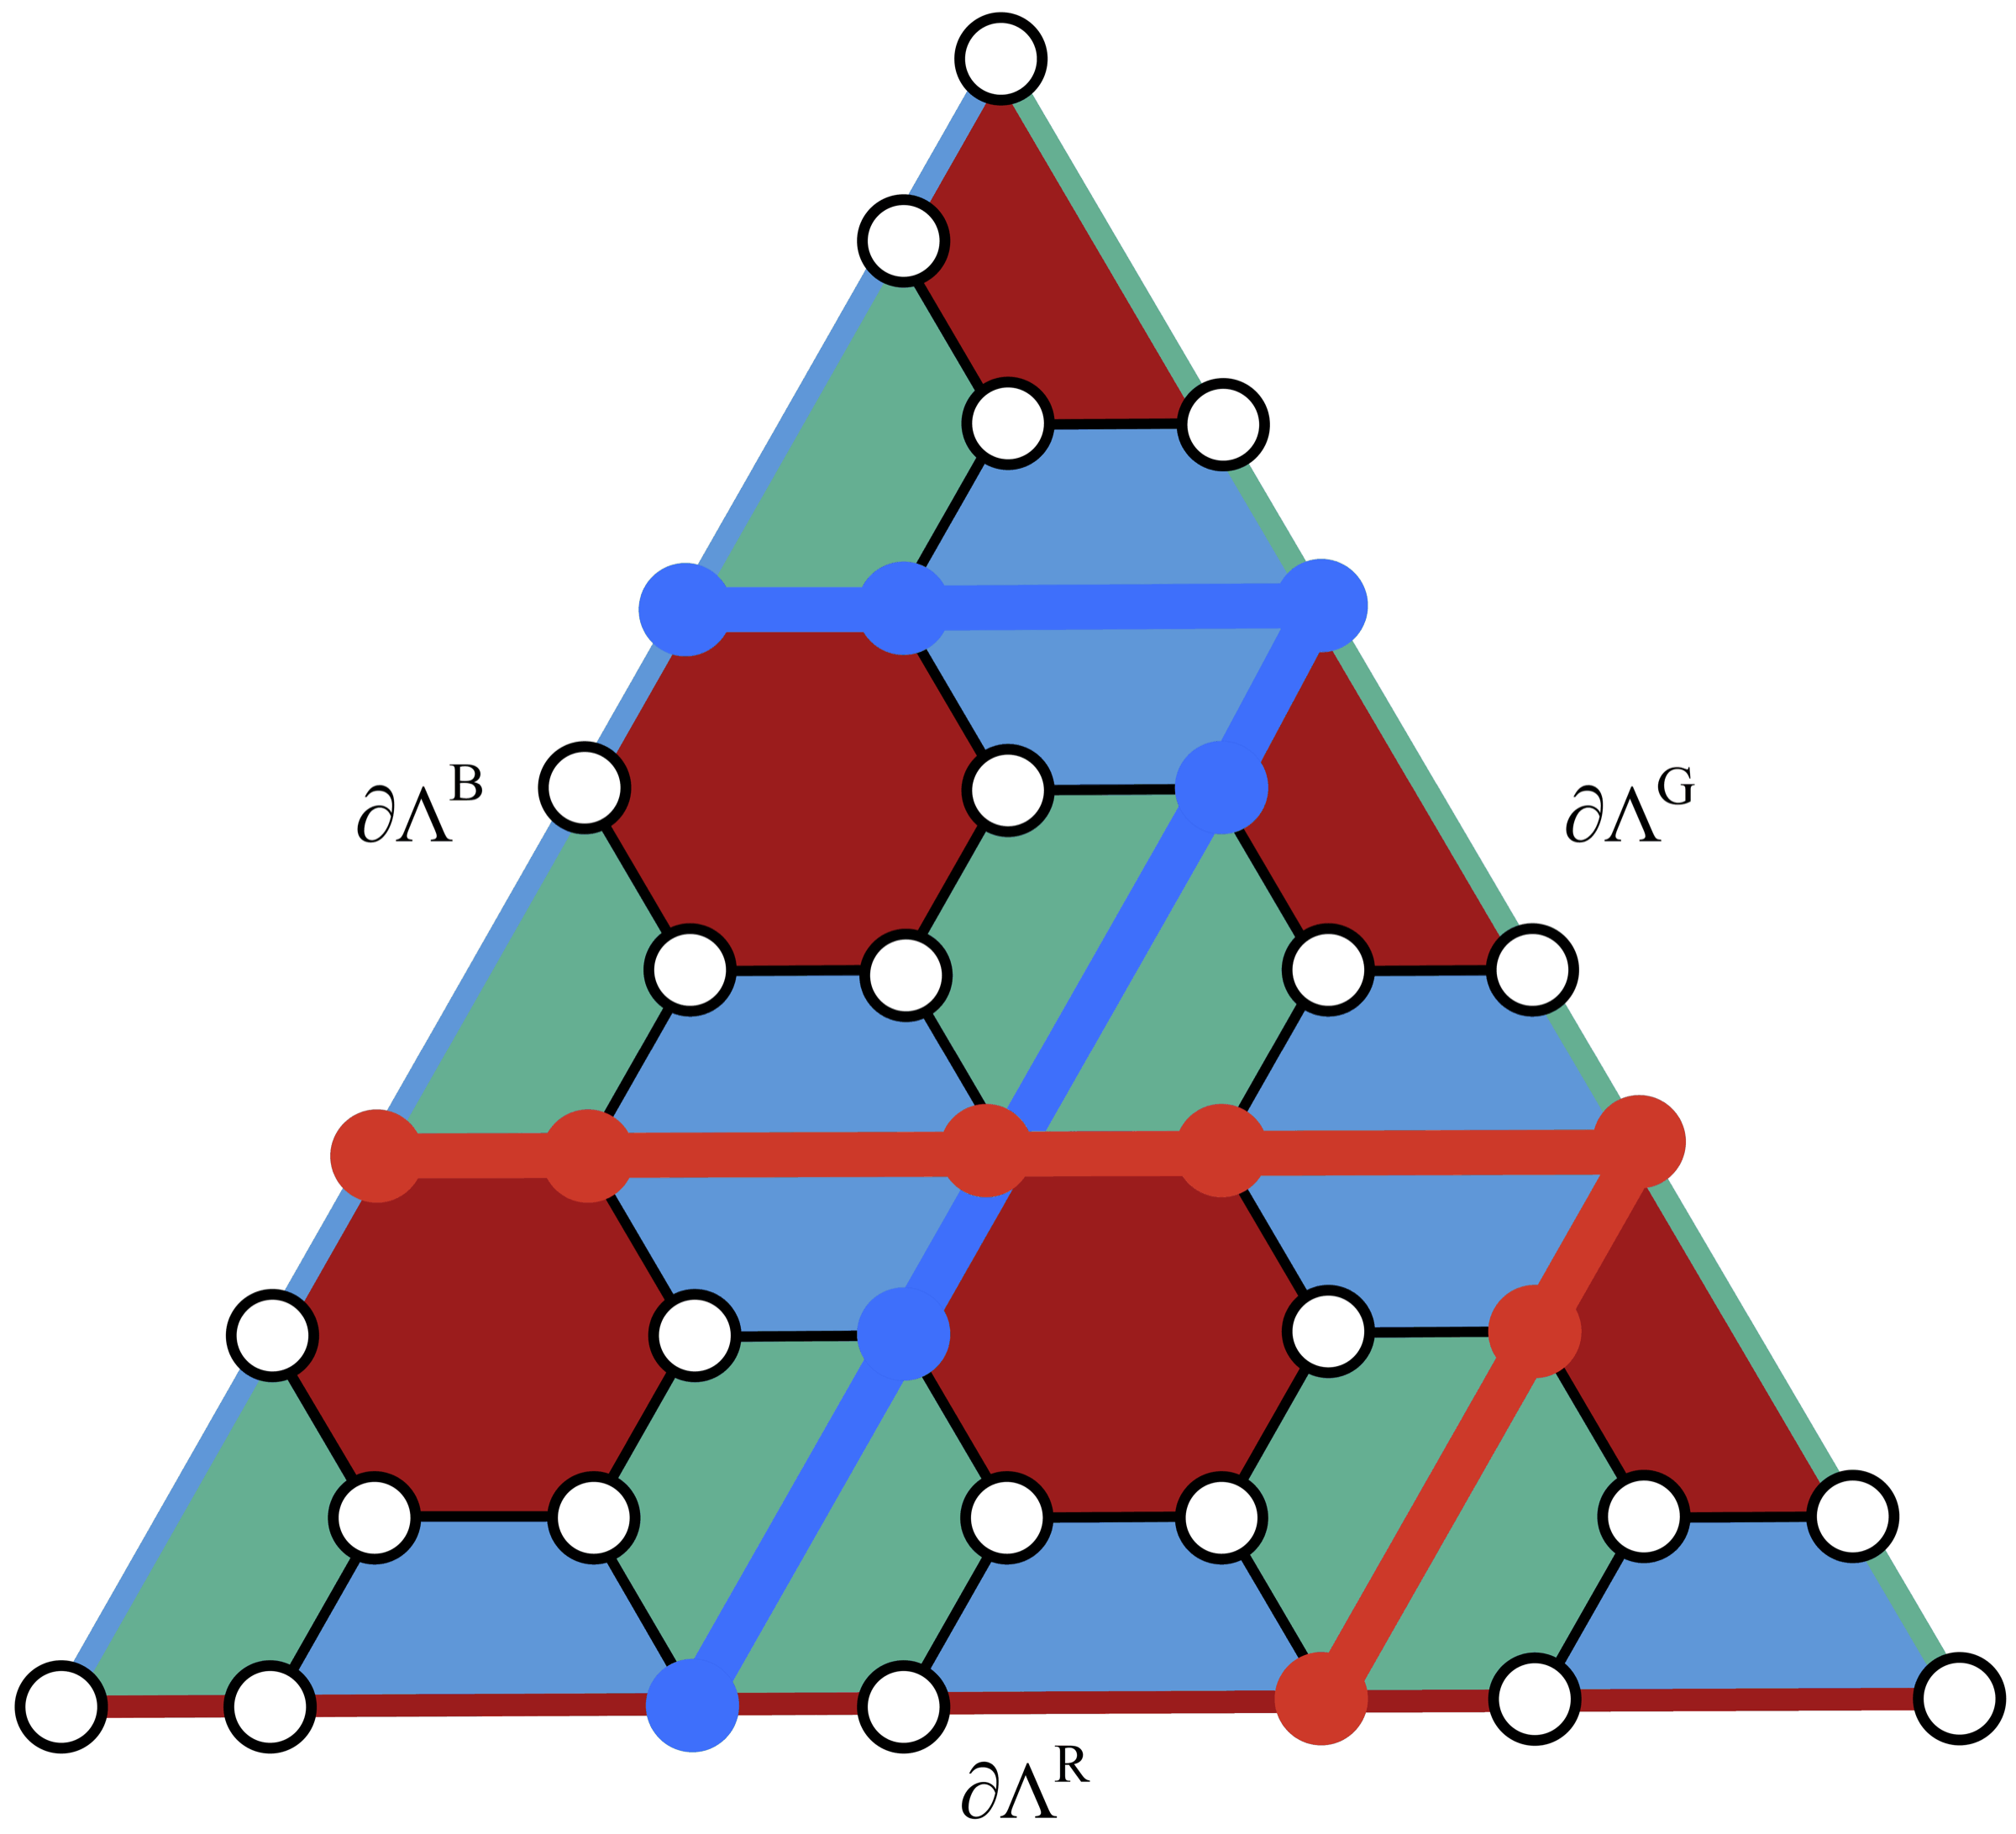
\includegraphics[width=0.4\textwidth]{triangle.png}
            \caption{Triangle code with three distinct boundaries. The logical operators $\overline{X}$ (red) and $\overline{Z}$ (blue) are strings of Pauli operators that touch every boundary. Notice that they intersect at a single point, and therefore anti-commute as expected.}
            \label{fig:x triangle}
        \end{figure}

A notable example of a color code is the triangle code, picture in Figure~\ref{fig:x triangle} which is a conveniently simple case. It is especially simple to  assign boundaries to this type of color code because it has only three boundaries, therefore each boundary is assigned a unique color in $\{R,G,B\}$. Therefore, for a triangle code defined on a lattice $\Lambda$, we can name its three boundaries $\partial\Lambda^R$, $\partial\Lambda^G$, and $\partial\Lambda^B$.\newline

The triangle code encodes one logical qubit, and admits a transversal logical Hadamard gate $\overline{H}$ and phase gate $\overline{R}_2$ \cite{kubica2014, kubica2015}. We will later study each of these in turn. The logical operators are defined as follows:
    \begin{itemize}
        \item \textbf{$\overline{Z}$}: a string of $\sigma^z$ that originates on boundary $\partial\Lambda^{\kappa_1}$, travels to $\partial\Lambda^{\kappa_2}$, and ends on $\partial\Lambda^{\kappa_3}$, for $\kappa_1\neq\kappa_2\neq\kappa_3$
        \item \textbf{$\overline{X}$}: a string of $\sigma^x$ that originates on boundary $\partial\Lambda^{\kappa_1}$, travels to $\partial\Lambda^{\kappa_2}$, and ends on $\partial\Lambda^{\kappa_3}$, for $\kappa_1\neq\kappa_2\neq\kappa_3$
    \end{itemize}
Essentially logical operators on the triangle code are strings of Pauli operators that touch every boundary.

\subsection{Folding in Two Dimensions}
The fact that topological color codes with boundaries admit transversal Hadamard gates $\overline{\mathcal{H}}$ poses a problem to the notion of equivalence. Namely, the toric code with two smooth and two rough boundaries does not admit $\mathcal{H}$, and therefore modifications need to be made to this toric code in order for equivalence to hold in the case with boundaries. The solution to this problem is achieved through process called \emph{folding} \cite{kubica2015}.
    \begin{definition}(Hadamard gate).
        \emph{The Hadamard operator $\mathcal{H}$ is a local unitary operator that exchanges Pauli $\sigma^x$ and $\sigma^z$ operators as follows:}
            \begin{align}
                \mathcal{H}\sigma^x\mathcal{H}^\dagger = \sigma^z,\enspace\enspace\enspace \mathcal{H}\sigma^z\mathcal{H}^\dagger = \sigma^x.
            \end{align}
        \emph{We may define the transversal Hadamard gate as the product of Hadamard operators over all qubits on the lattice:}
            \begin{align}
                \overline{\mathcal{H}} = \bigotimes_{v\in Q}\mathcal{H}_v.
    \end{align}
    \end{definition}
            \begin{figure}[h]
            \centering
            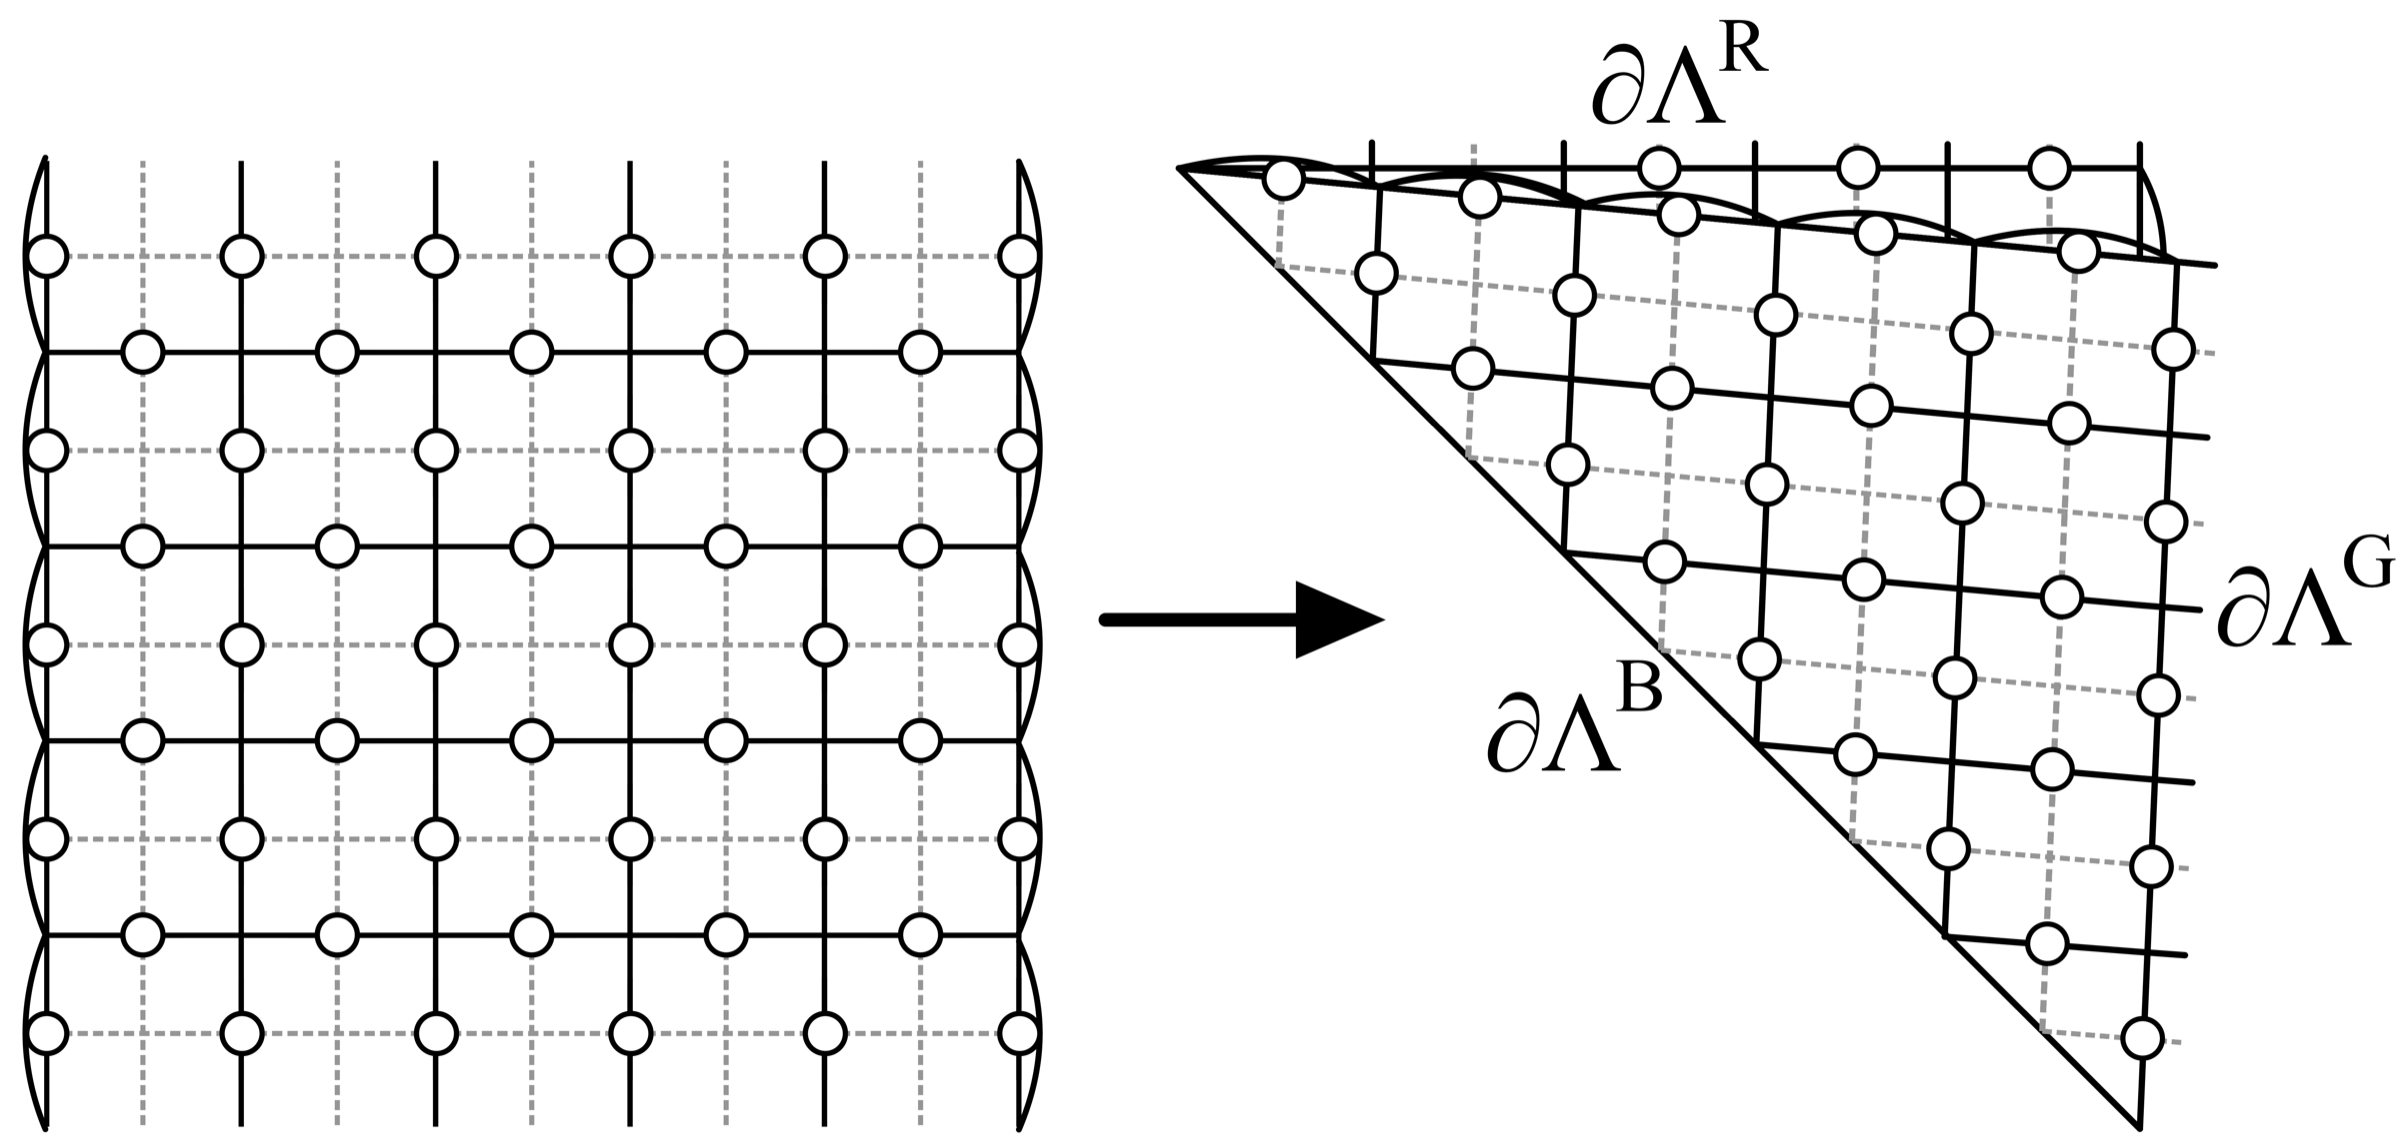
\includegraphics[width=0.4\textwidth]{folding.png}
            \caption{The folding process of a toric code with alternating boundary conditions.}
            \label{fig:x folding}
        \end{figure}
    \begin{claim}
        The toric code with two smooth and two rough boundaries does not admit the implementation of the transversal Hadamard gate $\overline{\mathcal{H}}$.
    \end{claim}
    \begin{proof}
        The toric code with boundaries encodes one logical qubit. The logical operators $\overline{Z}_{1,2}$ and $\overline{X}_{1,2}$ are associated to homologically non-trivial cycles on the lattice and dual lattice, respectively. Suppose $\overline{Z}_1$ and $\overline{Z}'_1$ are homologically equivalent. The action of the Hadamard gate on $\overline{Z}_1$, $\mathcal{H}\overline{Z}_1\mathcal{H}^\dagger$, must necessarily result in an object that anti-commutes with $\overline{X}'_1$. However, since $\overline{H}$ is local and unitary, $\mathcal{H}\overline{Z}_1\mathcal{H}^\dagger$ and $\overline{X}'_1$ do not overlap, and therefore commute. It follows that $\overline{\mathcal{H}}$ cannot be implemented in the toric code.
    \end{proof}

We now consider how the notion of shrunk lattices is modified for $\Lambda$ with boundaries. In the interior of the lattice nothing changes, and $\Lambda_R$ and $\Lambda_G$ result from shrinking plaquettes of colors $R$ and $G$, respectively. On the boundaries $\partial\Lambda^R$ and $\partial\Lambda^G$ we find the following:
    \begin{itemize}
        \item \textbf{$\partial\Lambda^R$}: $\Lambda_G$ has rough boundaries and $\Lambda_R$ has smooth boundaries
        \item \textbf{$\partial\Lambda^G$}: $\Lambda_R$ has rough boundaries and $\Lambda_G$ has smooth boundaries
    \end{itemize}
The disentangling operator does not affect the vertices on the boundary $\partial\Lambda^B$, and therefore the shrunk lattices $\partial\Lambda^R$ and $\partial\Lambda^G$ share the qubits on these vertices. Since $\Lambda_R$ and $\Lambda_G$ share qubits, they are attached along $\partial\Lambda^B$, and we are left with the lattice $\Lambda_R\#\Lambda_G$ with two smooth and two rough boundaries on which we can define the toric code $TC(\Lambda_R\#\Lambda_G)$. This is known as a \emph{folded} toric code, where $\Lambda_R\#\Lambda_G$ is obtained by attaching $\Lambda_R$ and $\Lambda_G$ along the boundary $\partial\Lambda^B$, see Figure~\ref{fig:x folding}. This folded toric code has three boundaries, $\partial\Lambda^R$, $\partial\Lambda^G$, and $\partial\Lambda^B$, and consists of two layers. We will adopt the convention where the 'top' layer consists of $\Lambda_R$, which has a rough boundary on $\partial\Lambda^G$ and a smooth boundary on $\partial\Lambda^R$. The 'bottom' layer consists of $\Lambda_G$, having a smooth boundary on $\partial\Lambda^G$ and a rough boundary on $\partial\Lambda^R$. This brings us to the following theorem:
    \begin{theorem}
        The triangular color code $CC(\Lambda)$ defined on a two-dimensional lattice $\Lambda$ with boundaries $\partial\Lambda^R$, $\partial\Lambda^G$, and $\partial\Lambda^B$, is equivalent to a folded toric code $TC(\Lambda_R\#\Lambda_G)$ defined on the lattice $\Lambda_R\#\Lambda_G$ with two smooth and two rough boundaries.
    \end{theorem}

\subsection{Quasiparticle Condensation on Boundaries}
Recall that in the toric code, electric charges condense on rough boundaries and magnetic vortices condense on smooth boundaries. The dyon $\epsilon = e\times m$ does not condense because it obeys fermionic statistics. Consider the folded toric code $TC(\Lambda_R\#\Lambda_G)$ defined in the previous section, obtained from attaching shrunk lattices $\Lambda_R$ and $\Lambda_G$ along the boarded $\partial\Lambda^B$. As previously mentioned, $TC(\Lambda_R\#\Lambda_G)$ has three boundaries and two layers ('top' and 'bottom'). Let $\{e_1,m_1,\epsilon_1\}$ and $\{e_2,m_2,\epsilon_2\}$ denote the toric code quasiparticles in the top and bottom layers, respectively. Having established the layer structure of $TC(\Lambda_R\#\Lambda_G)$, we can easily derive the following condensation mechanism on the folded toric code:
    \begin{itemize}
        \item $\partial\Lambda^R$ condenses $\{e_2,m_1,e_2m_1\}$
        \item $\partial\Lambda^G$ condenses $\{e_1,m_2,e_1m_2\}$
        \item $\partial\Lambda^B$ condenses $\{e_1e_2,m_1m_2,\epsilon_1\epsilon_2\}$
    \end{itemize}
This mechanism makes intuitive sense as, for example, $\partial\Lambda^R$ is smooth on the top layer - therefore condenses top-layer magnetic quasiparticles $m_1$ - and rough on the bottom layer - therefore condenses bottom-layer electric quasiparticles $e_2$.\newline

As this folded toric code is equivalent to a triangle code, we must also account for the color of the respective anyons, by noting that $e_\kappa$ and $m_\kappa$ can only condense on the boundary $\partial\Lambda^\kappa$ for $\kappa\in\{R,G,B\}$. Combining this with the fusion rules yields the following isomorphism between the anyons of the folded toric code and the color code:
    \begin{align}
        e_1\leftrightarrow e_R,\enspace\enspace\enspace e_2\leftrightarrow e_G,\enspace\enspace\enspace m_1\leftrightarrow m_G,\enspace\enspace\enspace m_2\leftrightarrow m_R
    \end{align}

\newpage\section{Three-Dimensional Color Codes}
\subsection{Equivalence Theorem in Three Dimensions}
In a three-dimensional lattice $\Lambda$, plaquettes enclose three-dimensional spaces known as \emph{volumes} that are four-colorable (with $R$, $G$, $B$, and $Y$). We will use $\mathcal{V}$ to denote the set of volumes on $\Lambda$, and $\{\mathcal{V}_\kappa\}_{\kappa\in\{R,G,B,Y\}}$ will denote the set of volumes of color $\kappa$. Plaquettes in three dimensions are adjacent to two volumes (one on each side), and edges are adjacent to three volumes. These objects are therefore colored as follows:
    \begin{itemize}
        \item Plaquettes are two-colorable: $RG$, $RB$, $RY$, $GB$, $GY$, and $BY$
        \item Edges are three-colorable: $RGB$, $RGY$, $RBY$, and $GBY$
    \end{itemize}

Qubits are still placed on vertices, however $\sigma^x$-type stabilizer are now associated to volumes (rather than plaquettes), while $\sigma^z$-type stabilizers are still associated to plaquettes. We defined these rigorously for clarity, noting that $\Pi(\nu)$ denoted the set of plaquettes that are adjacent to the volume $\nu\in\mathcal{V}$:
    \begin{align}
        \{Z_p\}_{p\in\Pi} = \prod_{v\in\mathcal{Q}(p)}\sigma^z_v,\enspace\enspace\enspace\{X_\nu\}_{\nu\in\mathcal{V}} = \prod_{p\in\Pi(\nu)}(\prod_{v\in\mathcal{Q}(p)}\sigma^x_v).
    \end{align}

We obtain shrunk lattices $\Lambda_R$, $\Lambda_G$, and $\Lambda_B$ by shrinking volumes of colors $R$, $G$, and $B$, respectively. More specifically, the structure of $\{\Lambda_{\kappa}\}_{\kappa\in\{R,G,B\}}$ consists of (for, $\beta,\gamma,\delta\in\{R,G,B,Y\}\setminus\{\kappa\}$):
    \begin{itemize}
        \item \textbf{Vertices}: centers of $\kappa$-colored volumes in $\Lambda$
        \item \textbf{Edges}: $\beta\gamma\delta$-colored edges in $\Lambda$
        \item \textbf{Plaquettes}: $\beta\gamma$, $\beta\delta$, and $\gamma\delta$ plaquettes in $\Lambda$
        \item \textbf{Volumes}: $\beta$, $\gamma$, and $\delta$ volumes in $\Lambda$
    \end{itemize}

Since in the three-dimensional case $|\Sigma| > |Q|$, the notion of \emph{ancilla qubits} must be introduced in order to match the dimensionalities of the Hilbert spaces $\mathcal{H}_Q = (\mathcal{H}_2)^{\otimes|Q|}$ and $\mathcal{H}_\Sigma = (\mathcal{H}_2)^{\otimes|\Sigma|}$. To this end, we define $\alpha = |\Sigma|-|Q|$ ancilla qubits with Hilbert space $\mathcal{H}_{ancilla}$ such that $\mathcal{H}_Q\otimes\mathcal{H}_{ancilla}\simeq\mathcal{H}_\Sigma$. Furthermore, we define the stabilizer group of the ancilla qubits $\mathcal{S}_{ancilla}$ as:
    \begin{align}
        \mathcal{S}_{ancilla} := \langle\{Z_{v_i}\}_{i\in\{1,...,\alpha\}}\rangle
    \end{align}

Toric codes defined on three-dimensional lattices are remarkably similar to their two-dimensional counterparts. Qubits are still placed on edges, boundary types are the same (i.e. rough and smooth), and we still have vertex and plaquette stabilizer operators $A_v$ and $B_p$.\newline

Theorem $3.1$ can be restated in three dimensions as follows:
    \begin{theorem}
        Let $CC(\Lambda)$ be a two-dimensional color code on a three-dimensional lattice $\Lambda$ without boundaries colored with $R$, $G$, $B$, and $Y$. There exists a local unitary Clifford transformation $U$, such that:
            \begin{align}
                U[CC(\Lambda)\otimes\mathcal{S}_{ancilla}]U^\dagger = TC(\Lambda_R)\otimes TC(\Lambda_G)\otimes TC(\Lambda_B),
            \end{align}
        where $TC(\Lambda_R)$, $TC(\Lambda_G)$ and $TC(\Lambda_B)$ are three independent toric codes on the shrunk lattices $\Lambda_R$, $\Lambda_G$ and $\Lambda_B$. Furthermore, one can write:
            \begin{align}
                U = \bigotimes_{\nu\in \mathcal{V}_Y}U_\nu,
            \end{align}
        where $U_\nu$ is a unitary Clifford transformation acting on the qubits surrounding the $Y$-colored volumes $\mathcal{Q}(\Pi(\nu))$.
    \end{theorem}

We require the local unitary Clifford transformation:
    \begin{align}
        \{U_\nu\}_{\nu\in\mathcal{V}_Y} = \bigotimes_{p\in\Pi(\nu)}U_p,
    \end{align}
to act as follows:
    \begin{align}
        \{\sigma^z_{v_i}\sigma^z_{v_{i+1}}\}_{i\in\{1,...,2n-1\}}&\xrightarrow{U_p}Z_{e|\partial_1e := \{v_i,v_{i+1}\}}\\
        X_p&\xrightarrow{U_p}\prod_{e|v\in\partial_1e\;\text{and}\;e\notin\partial_2p}\sigma^x_e.
    \end{align}
One can verify that these mappings send:
    \begin{itemize}
        \item $\{X_p\}_{p\in\Pi(\nu)|\nu\in\mathcal{V}_\kappa}$ volume stabilizers in $CC(\Lambda)$ to $\{A_v\}_{v\in V}$ vertex stabilizers in $TC(\Lambda_\kappa)$ for $\kappa\in\{R,G,B\}$
        \item $\{Z_p\}_{p\in\Pi}$ plaquette stabilizers of colors $GB$, $GY$, and $BY$ in $CC(\Lambda)$ to $\{B_p\}_{p\in P}$ plaquette stabilizers in $TC(\Lambda_R)$
        \item $\{Z_p\}_{p\in\Pi}$ plaquette stabilizers of colors $RB$, $RY$, and $BY$ in $CC(\Lambda)$ to $\{B_p\}_{p\in P}$ plaquette stabilizers in $TC(\Lambda_G)$
        \item $\{Z_p\}_{p\in\Pi}$ plaquette stabilizers of colors $RG$, $RY$, and $GY$ in $CC(\Lambda)$ to $\{B_p\}_{p\in P}$ plaquette stabilizers in $TC(\Lambda_B)$
    \end{itemize}

To define $\{U_\nu\}_{\nu\in\mathcal{V}_Y}$ more rigorously, we consider the overlap group of $CC(\Lambda)$ on $\nu_Y\in\mathcal{V}_Y$. Intuitively, this is the group generated as follows:
    \begin{align}
        \mathcal{O}_{\nu_Y} = \langle\{\sigma^z_{v_i}\sigma^z_{v_{i+1}}\}_{i\in\{1,...,2n\}}, \{X_p\}_{p\in\Pi(\nu_Y)}\rangle.
    \end{align}
The objective is to construct $\{U_\nu\}_{\nu\in\mathcal{V}_Y}$ such that it maps the group $\mathcal{O}_{\nu_Y}\otimes\Lambda_{ancilla}$ to the overlap group of the three-dimensional toric code $\mathcal{O}_{p_R\cup p_G\cup p_B}$ which, for $p\in \Pi_R\cup \Pi_G\cup \Pi_B$, is defined:
    \begin{align}
        \mathcal{O}_{p_R\cup p_G\cup p_B} := \langle\{\sigma^z_e\}_{e\in\partial_2p},\sigma^x_{e\notin\partial_2p|\partial_1e\cap\partial_1e'\neq\emptyset\;\text{for}\; e'\in\partial_2p}\rangle .
    \end{align}
We can see that the transformations $(2.1.5)$ and $(2.1.6)$ map the elements in $Z(\mathcal{O}_{\nu_Y}\otimes\mathcal{L})$ to $Z(\mathcal{O}_{p_R\cup p_G\cup p_B})$. Let us define these centralizers:
    \begin{align}
        Z(\mathcal{O}_{\nu_Y}) &= \langle\{Z_p\}_{p\in\Pi},\{X_p\}_{p\in\Pi},\{\sigma^z_{v_i}\}_{i\in\{1,...,2n\}}\rangle\\
        Z(\mathcal{O}_{p_R\cup p_G\cup p_B}) &= \langle\prod_{e|\partial_1e := \{v_i,v_j\}}\sigma^z_e\;\text{for}\;i\in\{1,3,5,...,2n-1\}\;\text{and}\;j\in\{2,4,6,...,2n\}\rangle .
    \end{align}
It is important to note that the generators of $U(CC(\Lambda)\otimes_{\nu\in\mathcal{V}_Y}[\mathcal{S}_{ancilla}]_{\nu_Y})U^\dagger$ are supported on either $\Lambda_R$, $\Lambda_G$, or $\Lambda_B$, thus one can indeed obtain three decoupled copies of the toric code.
    \begin{claim}
        $\mathcal{O}_{\nu_Y}$ and $\mathcal{O}_{p_R\cup p_G\cup p_B}$ are isomorphic.
    \end{claim}
    \begin{proof}
        Let $N = |\Sigma|$, $M = |Q|$, $F = |\Pi|$. It is easy to see that $\mathcal{O}_{\nu_Y},\mathcal{O}_{p_R\cup p_G\cup p_B}\subset\textbf{Pauli}(N)$. We proceed by first labeling the generators of $\mathcal{O}_{p_R\cup p_G\cup p_B}$ and $\mathcal{O}_{\nu_Y}$.\newline

        The generators $\{\sigma^z_{v_i}\sigma^z_{v_{i+1}}\}_{i\in\{1,...,2n\}}$ of $\mathcal{O}_{\nu_Y}$ are supported on the edges of $\Lambda$, therefore there are $M - 1$ such independent operators. The generators $\{X_p\}_{p\in\Pi(\nu)}$  are supported on three types of plaquettes, namely those of colors $RY$, $GY$, and $BY$, therefore there are $F-3$ such independent operators (we must remove one for each type of plaquette). We also have an $\sigma^x$-type volume generator of the form $\prod_{p\in\Pi(\nu_Y)}X_p$. Finally, we must account for the $\sigma^z$-type stabilizer generators on the $\alpha$ ancilla qubits (recall $\alpha = N - M$). We may therefore label the generators of $\mathcal{O}_{\nu_Y}$ with $\{g_i\}_{i\in\{1,...,N+F-3\}}$ as follows:
            \begin{itemize}
                \item $\{g_i\}_{i\in\{1,...,M-1\}}$ correspond to the $\sigma^z_{v_i}\sigma^z_{v_{i+1}}$ operators defined on adjacent vertices
                \item $\{g_i\}_{i\in\{M,...,M+F-4\}}$ correspond to the $X_p$ plaquette operators
                \item $g_{M+F-3}$ corresponds to the $\prod_{p\in\Pi(\nu_Y)}X_p$ volume operator on $\nu\in\mathcal{V}_Y$
                \item $\{g_i\}_{i\in\{M+F-2,...,N+F-3\}}$ correspond to the Pauli $\sigma^x$ operators defined on the ancilla qubits
            \end{itemize}
        We have therefore labeled all $N+F-3$ independent generators of $\mathcal{O}_{\nu_Y}$. It follows that $Z(\mathcal{O}_{\nu_Y})$ has $(F-2)+1+(N-M) = F+N-M-1$ independent generators.

        The $\{\sigma^z_e\}_{e\in\partial_2p}$ generators of $\mathcal{O}_{p_R\cup p_G\cup p_B}$ are defined on the edges of the toric lattice, so there are $N$ such independent generators. Similarly to the reasoning for $\mathcal{O}_{\nu_Y}$, the generators $\sigma^x_{e\notin\partial_2p|\partial_1e\cap\partial_1e'\neq\emptyset\;\text{for}\; e'\in\partial_2p}$ are associated to three types of colored plaquettes: $RY$, $GY$, and $BY$, so there are $F-3$ such generators. We label these generators with $\{h_i\}_{i\in\{1,...,N+F-3\}}$ defined as follows:
            \begin{itemize}
                \item $\{h_i\}_{i\in\{1,...,N\}}$ correspond to the Pauli $\sigma^x$ operators defined on edges
                \item $\{h_i\}_{i\in\{N+1,...,N+F-3\}}$ correspond to the $\sigma^x_{e\notin\partial_2p|\partial_1e\cap\partial_1e'\neq\emptyset\;\text{for}\; e'\in\partial_2p}$ operators defined on the edges incident on plaquettes 
            \end{itemize}
        In total, we obtain $E+F-3$ generators of $\mathcal{O}_{p_R\cup p_G\cup p_B}$, and $2F-3$ independent generators of $Z(\mathcal{O}_{p_R\cup p_G\cup p_B})$.

        Using the Euler characteristic, we may calculate $G(Z(\mathcal{O}_{\nu_Y}))$ and $G(Z(\mathcal{O}_{p_R\cup p_G\cup p_B}))$ explicitly. We find that $G(Z(\mathcal{O}_{\nu_Y})) = G(Z(\mathcal{O}_{p_R\cup p_G\cup p_B})) = 2$, therefore by Lemma $3.4$, $\mathcal{O}_{\nu_Y}$ and $\mathcal{O}_{p_R\cup p_G\cup p_B}$ are isomorphic.
    \end{proof}
Furthermore, it can be verified that $\{g_i\}$ and $\{h_i\}$ have the same commutation relations. From Lemma $3.5$, it follows that there exists a local unitary Clifford transformation $U_{\nu_Y}$ such that:
            \begin{align}
                U_{\nu_Y} g_iU^\dagger_{\nu_Y} = h_i\enspace\forall\enspace i\in\{1,...,N+F-3\}.
            \end{align}

\subsection{Folding in Three Dimensions}
We have already defined the total boundary of a color code defined on a lattice $\Lambda$ as:
    \begin{align}
        \partial\Lambda = \bigcup^n_{i = 1}\partial\Lambda^i ,
    \end{align}
where each $\partial\Lambda^i$ is assigned a color. In three dimensions, each boundary is assigned a color in $\{R,G,B,Y\}$, and we say that $\partial\Lambda^i$ is of color $\kappa\in\{R,G,B,Y\}$ if all volumes adjacent to $\partial\Lambda^i$ have colors in $\{R,G,B,Y\}\setminus\{\kappa\}$.\newline

In order to study the folding mechanism in three dimensions, we will focus on the three-dimensional counterpart of the triangle code. This is a color code $CC(\Lambda)$ defined on a tetrahedral lattice $\Lambda$, which we will refer to as the tetrahedral code for simplicity. It is easy to see that this lattice has four boundaries, one of each color: $\partial\Lambda^R$, $\partial\Lambda^G$, $\partial\Lambda^B$, and $\partial\Lambda^Y$.\newline

Intuitively, when we apply the disentangling operator $U = \bigotimes_{\nu\in\mathcal{V}_Y}U_\nu$ to this tetrahedral code, we will obtain a toric code defined on the lattice $\Lambda_R\#\Lambda_G\#\Lambda_B$ obtained from attaching the shrunk lattices $\Lambda_R$, $\Lambda_G$, and $\Lambda_B$ along the boundary $\partial\Lambda^Y$. Formally:
    \begin{align}
        U[CC(\Lambda)\otimes\mathcal{S}_{ancilla}]U^\dagger = TC(\Lambda_R\#\Lambda_G\#\Lambda_B).
    \end{align}\newpage
This can be generalized to $d$ dimensions:
    \begin{theorem}
        Let $CC(\Lambda)$ be a color code defined on a $d$ simplex lattice $\Lambda$, with $d+1$ boundaries $\{\partial\Lambda^i\}_{i\in\{0,...,d\}}$, each assigned a unique color from $\{\kappa_0,...,\kappa_d\}$. There exists a local unitary Clifford transformation $U = \prod_{\theta\in\Theta_{\kappa_0}}U_\theta$ such that:
            \begin{align}
                U[CC(\Lambda)\otimes\mathcal{S}_{ancilla}]U^\dagger = TC(\#^d_{i = 1}\Lambda_i),
            \end{align}
        where $\Theta_{\kappa_0}$ represents the set of $d+1$ cells in $\Lambda$ of color $\kappa_0$. The lattice $\#^d_{i = 1}\Lambda_i$ is obtained by attaching the shrunk lattices $\{\Lambda_i\}_{i\in\{1,...,d\}}$ along the boundary $\partial\Lambda^0$.
    \end{theorem}

\subsection{Transversal Gates}
\subsubsection{The Hadamard Gate}
Recall definition $(3.9)$ for the transversal Hadamard gate. It is trivial to see that $H_{CC}$ is invariant under conjugation by the transversal Hadamard gate \cite{yoshida2015}:
    \begin{align}
        \overline{\mathcal{H}}H_{CC}\overline{\mathcal{H}}^\dagger = H_{CC}.
    \end{align}
Furthermore, $\overline{\mathcal{H}}$ transforms $\overline{X^{\kappa_1\kappa_2}}(\gamma_{\kappa_1\kappa_2})$ operators into $\overline{X^{\kappa_1\kappa_2}}(\gamma_{\kappa_1\kappa_2})$ operators and vice versa:
    \begin{align}
        \{e_\kappa\}_{\kappa\in\{R,G,B\}}&\xrightarrow{\overline{\mathcal{H}}}m_\kappa\\
        \{m_\kappa\}_{\kappa\in\{R,G,B\}}&\xrightarrow{\overline{\mathcal{H}}}e_\kappa.
    \end{align}

\subsubsection{The Phase Gate}
As previously mentioned, color codes also admit the $d$-dimensional phase operator $R_d$:
    \begin{align}
        R_d = \text{diag}(1,e^{\frac{i\pi}{2^{d-1}}}).
    \end{align}
We note that $R_2$ has the following action on the Pauli $\sigma^x$, $\sigma^x\sigma^z$, and $\sigma^z$ operators:
    \begin{align}
        R_2\sigma^xR^\dagger_2 = \sigma^x\sigma^y,\enspace\enspace\enspace R_2\sigma^x\sigma^zR^\dagger_2 = -\sigma^x,\enspace\enspace\enspace R_2\sigma^zR^\dagger_2 = \sigma^z.
    \end{align}
In order to construct the transversal phase operator, we must define the notion of a bipartite graph.
    \begin{definition}(Bipartite graph).
        \emph{A graph $G(V,E)$ is said to be bipartite if and only if there exist $V_1,V_2\subseteq V$ such that $V = V_1\cup V_2$, $V_1\cap V_2 = \emptyset$, and each $e\in E$ has one endpoint in $V_1$ and one in $V_2$.}
    \end{definition}
It is intuitively clear that $\Lambda(Q,\Sigma)$ is bipartite, but we wish to prove this rigorously. To do this, we must introduce some facts from graph theory \cite{kubica2014}.
    \begin{definition}(Even cycle).
        \emph{An even cycle on a graph $G(V,E)$ is a closed path on $G$ that traverses an even number of edges. In the language of algebraic topology, an even cycle is a $1$-cycle $c\in Z_1$ that contains an even number of edges.}
    \end{definition}
    \begin{lemma}
        A graph $G(V,E)$ containing only even cycles is bipartite.
    \end{lemma}
    \begin{claim}
        The lattice $\Lambda(Q,\Sigma)$ on which we define the color code, is bipartite.
    \end{claim}
    \begin{proof}
        We have already established that all plaquettes in $\Lambda(Q,\Sigma)$ have an even number of edges, and each cycle on $\Lambda(Q,\Sigma)$ is contractible. Therefore all cycles on $\Lambda(Q,\Sigma)$ form the boundary of a group plaquettes, and must contain an even number of edges. Thus by Lemma $3.3$, $\Lambda(Q,\Sigma)$ is bipartite
    \end{proof}
We can therefore split the qubits in $\Lambda$ into complementary sets $T$ and $T^c = Q\setminus T$ such that $Q = T\cup T^c$. On a topological color code $CC(\Lambda)$ defined on a $d$-dimensional lattice $\Lambda$, the transversal phase operator $\overline{R_d}$ is defined:
    \begin{align}
        \overline{R_d} = \bigotimes_{v\in T}[R_d]_v\bigotimes_{v\in T^c}\frac{1}{[R_d]_v},
    \end{align}
where $[R_d]_v$ represents the application of the $d$-dimensional phase operator on the vertex $v\in Q$. Ground state configurations are invariant under the application of $\overline{R_2}$. Furthermore, the two dimensional transversal phase operator implements the following anyon exchanges:
    \begin{align}
        e_R\rightarrow e_R,\enspace\enspace\enspace e_G\rightarrow e_G\\
        m_R\rightarrow m_Re_R,\enspace\enspace\enspace m_G\rightarrow m_Ge_G.
    \end{align}
This makes sense considering the actions of the disentangling operator defined above. We saw that $\sigma^z$ operators are invariant under the action of $R_2$, therefore it it perfectly logical that electric excitations, being strings of $\sigma^z$ operators, remain unchanged. On the other hand, $R_2$ maps $\sigma^x$ operators to $\sigma^x\sigma^z$, so once again we find consistency with our definitions.\newline

Consider a three-dimensional color code $CC(\Lambda)$ defined on a cube-like lattice $\Lambda$ with colors $R$, $G$, $B$, and $Y$. We construct $\Lambda$ such that opposite boundaries have the same color, and we set a coordinate system with basis $\{\hat{g}, \hat{b}, \hat{y}\}$ such that the two boundaries that are perpendicular to the $\hat{g}$ direction are colored with $G$. Similarly, the two boundaries perpendicular to the $\hat{b}$ direction have color $B$, and the two boundaries perpendicular to $\hat{y}$ have color $Y$. The action of the disentangling operator $U = \prod_{\nu\in\mathcal{V}_Y}U_\nu$ is as follows:
    \begin{align}
        U[CC(\Lambda)\otimes\mathcal{S}_{ancilla}]U^\dagger = \bigotimes_{\kappa\in\{R,G,B\}}TC(\Lambda_\kappa),
    \end{align}
where $\{\Lambda_\kappa\}_{\kappa\in\{R,G,B\}}$ is the shrunk lattice obtained by shrinking the volumes in $\Lambda$ of color $\kappa$. More specifically, $\{\Lambda_\kappa\}_{\kappa\in\{R,G,B\}}$ is cube-like with two rough and two smooth boundaries; the rough boundaries are those that are perpendicular to the $\hat{\kappa}\in\{\hat{r},\hat{g},\hat{b}\}$ direction. Since $\{\Lambda_\kappa\}_{\kappa\in\{G,B,Y\}}$ clearly encodes one logical qubit, and $CC(\Lambda)$ is equivalent to three decoupled copied of this kind of toric code, then $CC(\Lambda)$ encoded three logical qubits. This is a remarkable result.\newline

Since $\overline{R_3}^2 = \II$, in this construction $\overline{R_3}$ does not implement logical $R_3$ gates in the code space. However, it turns out that $\overline{R_3}$ implements the logical $CCZ$ gate on three stacked copies of the toric code, which we will study in detail in the next section.

\subsubsection{The $C^{\otimes d-1}Z$ Gate}
Let us first work on a color code $CC(\Lambda)$ defined on a two-dimensional square-like lattice where, as in the previous section, opposite boundaries have the same color (the code has colors $R$, $G$, and $B$). Since $CC(\Lambda)$ can be disentangled into two decoupled copies of the toric code, this color code encodes two logical qubits. We denote the logical operators of the color code with $\overline{X}^{1,2}_{CC}$ and $\overline{Z}^{1,2}_{CC}$, where $\overline{X}^1_{CC}$, $\overline{Z}^2_{CC}$ are vertical, and $\overline{X}^2_{CC}$, $\overline{Z}^1_{CC}$ are horizontal. For simplicity, we will maintain the previous notation for the logical operators on toric codes, $\overline{X}_{1,2}$, $\overline{Z}_{1,2}$, where $\overline{Z}_1$, $\overline{X}_2$ are vertical and $\overline{Z}_2$, $\overline{X}_1$ are horizontal. Since $R_2\sigma^xR^\dagger_2 = \sigma^x\sigma^z$, the transversal phase operator has the following action on the logical operators:
    \begin{align}
        \overline{X}^1_{CC}&\rightarrow\overline{X}^1_{CC}\overline{Z}^2_{CC}\\
        \overline{Z}^1_{CC}&\rightarrow\overline{Z}^1_{CC}\\
        \overline{X}^2_{CC}&\rightarrow\overline{Z}^1_{CC}\overline{X}^2_{CC}\\
        \overline{Z}^2_{CC}&\rightarrow\overline{Z}^2_{CC}.
    \end{align}
As mentioned above, $CC(\Lambda)$ disentangles into two decoupled copies of the toric code $TC(\Lambda_R)\otimes TC(\Lambda_G)$ under the action of $U = \bigotimes_{p\in\Pi_B}U_p$. The disentangling operator $U$ therefore defines the following isomorphism:
    \begin{align}
        \overline{X}^1_{CC}&\leftrightarrow\overline{X}_1\otimes\II\\
        \overline{X}^2_{CC}&\leftrightarrow\II\otimes\overline{X}_2\\
        \overline{Z}^1_{CC}&\leftrightarrow\overline{Z}_1\otimes\II\\
        \overline{Z}^2_{CC}&\leftrightarrow\II\otimes\overline{Z}_2,
    \end{align}
where $\overline{X}_{1,2}$ and $\overline{Z}_{1,2}$ denote the logical operators of the decoupled toric codes. Remarkably, by applying the disentangling operator to the transversal phase gate - $U\overline{R_2}U^\dagger$ - we can consider the action of the resulting object on $TC(\Lambda_R)\otimes TC(\Lambda_G)$:
    \begin{align}
        \overline{X}_1\otimes\II&\rightarrow\overline{X}_1\otimes\overline{Z}_2\\
        \II\otimes\overline{X}_2&\rightarrow\overline{Z}_1\otimes\overline{X}_2\\
        \overline{Z}_1\otimes\II&\rightarrow\overline{Z}_1\otimes\II\\
        \II\otimes\overline{Z}_2&\rightarrow\II\otimes\overline{Z}_2.
    \end{align}

We turn our attention to a three-dimensional color code $CC(\Lambda)$ defined on a cube-like lattice $\Lambda$ with colors $\{R,G,B,Y\}$ and coordinate basis $\{\hat{r},\hat{g},\hat{b}\}$. The boundaries perpendicular to the direction $\hat{\kappa}\in\{\hat{r},\hat{g},\hat{b}\}$ have color $\kappa\in\{R,G,B\}$, so opposite boundaries have the same color. By now it is clear that as a consequence of the equivalence theorem $CC(\Lambda)$ encodes three logical qubits. We will label the logical operators $\overline{X}^{1,2,3}_{CC}$ and $\overline{Z}^{1,2,3}_{CC}$.\newline

The $3$-qubit control-$Z$ gate $CCZ$ is the three-dimensional implementation of the control-$Z$ gate. Let $|x_1x_2x_3\rangle$ denote the computational basis on $CC(\Lambda)$, then the action of $CCZ$ can be defined:
    \begin{align}
        CCZ|x_1x_2x_3\rangle = (-1)^{x_1x_2x_3}|x_1x_2x_3\rangle .
    \end{align}
We continue by computing some important commutation relations, where $[A,B] = ABA^\dagger B^\dagger$:
    \begin{align}
        [CCZ,\sigma^x\otimes\II\otimes\II]|x_1x_2x_3\rangle &= CCZ(\sigma^x\otimes\II\otimes\II)CCZ^\dagger(\sigma^x\otimes\II\otimes\II)^\dagger|x_1x_2x_3\rangle\\
        &= CCZ(\sigma^x\otimes\II\otimes\II)CCZ(\sigma^x\otimes\II\otimes\II)|x_1x_2x_3\rangle\\
        &= CCZ(\sigma^x\otimes\II\otimes\II)CCZ|\sigma^x(x_1)x_2x_3\rangle\\
        &= CCZ(\sigma^x\otimes\II\otimes\II)(-1)^{\sigma^x(x_1)x_2x_3}|\sigma^x(x_1)x_2x_3\rangle\\
        &= CCZ(-1)^{\sigma^x(x_1)x_2x_3}|x_1x_2x_3\rangle\\
        &= (-1)^{x_1x_2x_3}(-1)^{\sigma^x(x_1)x_2x_3}|x_1x_2x_3\rangle\\
        &= (-1)^{(x_1+\sigma^x(x_1))x_2x_3}|x_1x_2x_3\rangle,
    \end{align}
If $|x_1\rangle = |0\rangle$, then $\sigma^x|x_1\rangle = |1\rangle$, and $x_1+\sigma^x(x_1) = 0+1 = 1$. If If $|x_1\rangle = |1\rangle$, then $\sigma^x|x_1\rangle = |0\rangle$, and $x_1+\sigma^x(x_1) = 1+0 = 1$. So no matter what state $|x_1\rangle$ is in, we find that $x_1+\sigma^x(x_1) = 1$. Then:
    \begin{align}
        [CCZ,\sigma^x\otimes\II\otimes\II]|x_1x_2x_3\rangle &= (-1)^{(x_1+\sigma^x(x_1))x_2x_3}|x_1x_2x_3\rangle\\
        &= (-1)^{x_2x_3}|x_1x_2x_3\rangle\\
        &= \II\otimes CZ|x_1x_2x_3\rangle\\
        [CCZ,\sigma^x\otimes\II\otimes\II] &= \II\otimes CZ.
    \end{align}
There is another important commutator to compute:
    \begin{align}
        [R_3,\sigma^x] &= R_3\sigma^xR^\dagger_3(\sigma^x)^\dagger\\
        &= R_3\sigma^xR_3\sigma^x\\
        &= \begin{pmatrix}
            1 & 0 \\
            0 & e^{\frac{i\pi}{4}}
            \end{pmatrix}
            \begin{pmatrix}
            0 & 1 \\
            1 & 0
            \end{pmatrix}
            \begin{pmatrix}
            1 & 0 \\
            0 & e^{-\frac{i\pi}{4}}
            \end{pmatrix}
            \begin{pmatrix}
            0 & 1 \\
            1 & 0
            \end{pmatrix}\\
        &= \begin{pmatrix}
            0 & 1 \\
            e^{\frac{i\pi}{4}} & 0
            \end{pmatrix}
            \begin{pmatrix}
            0 & 1 \\
            e^{-\frac{i\pi}{4}} & 0
            \end{pmatrix}\\
        &= \begin{pmatrix}
            e^{-\frac{i\pi}{4}} & 0 \\
            0 & e^{\frac{i\pi}{4}}
            \end{pmatrix}\\
        &= e^{-\frac{i\pi}{4}}
            \begin{pmatrix}
            1 & 0 \\
            0 &  e^{\frac{i\pi}{2}}
            \end{pmatrix}\\
        &= e^{-\frac{i\pi}{4}}R_2 .
    \end{align}
These relations can be used to define $\overline{R_3}$ recursively:
    \begin{align}
        \overline{R_2} &= [\overline{R_3}, \overline{X}^1_{CC}]\\
        \overline{R_1} &= [\overline{R_2}, \overline{X}^2_{CC}] = \overline{Z}^3_{CC} .
    \end{align}
We can therefore implement the logical $CCZ$ gate on a stack of 3 copies of the toric code by using the e traversal phase gate $\overline{R_3}$:
    \begin{align}
        \II\otimes\overline{CZ}&\propto[\overline{CCZ},\overline{X}_1]\\
        \II\otimes\II\otimes\overline{Z}&\propto[\II\otimes\overline{CZ},\overline{X}_2].
    \end{align}
These relations allow us to find an isomorphism between the logical operators of the color code and the toric code:
    \begin{align}
        \overline{X}^1_{CC}\leftrightarrow\overline{X}_1,\enspace\enspace\enspace \overline{Z}^1_{CC}\leftrightarrow\overline{Z}_1.
    \end{align}
We can generalize these notions to $d$ dimensions. For a color code $CC(\Lambda)$ defined on a $d$-dimensional hypercube-like lattice with colors $\{\kappa_0,...,\kappa_d\}$ and logical operators $\{\overline{X}^i_{CC}\}_{i\in\{1,...,d\}},\newline \{\overline{Z}^i_{CC}\}_{i\in\{1,...,d\}}$ defined such that $\overline{Z}^i_{CC}$ is parallel to direction $\hat{i}$ and $\overline{X}^i_{CC}$ is perpendicular to $\hat{i}$. In $d$-dimensions, the recursive relations $(184)-(185)$ become \cite{kubica2015}:
    \begin{align}
        \overline{R_{d-1}} &= [\overline{R_d}, \overline{X}^1_{CC}]\\
        \overline{R_{d-2}} &= [\overline{R_{d-1}}, \overline{X}^2_{CC}]\\
        &\enspace\vdots\\
        \overline{R_1} &= [\overline{R_2}, \overline{X}^{d-1}_{CC}] = \overline{Z}^d_{CC}.
    \end{align}
And:
    \begin{align}
        \II\otimes\overline{C^{\otimes d-2}Z}&\propto [\overline{C^{\otimes d-1}Z}, \overline{X}^1_{CC}]\\
        \II\otimes\II\otimes\overline{C^{\otimes d-3}Z}&\propto [\II\otimes\overline{C^{\otimes d-2}Z}, \overline{X}^2_{CC}]\\
        &\enspace\vdots\\
        \II^{\otimes d-1}\otimes\overline{Z}&\propto [\overline{CZ}, \overline{X}^{d-1}_{CC}].
    \end{align}
This brings us to the following important theorem:
    \begin{theorem}
        Let $CC(\Lambda)$ be a $d$-dimensional color code defined on a hypercube-like lattice $\Lambda$ with colors $\{\kappa_0,...,\kappa_{d}\}$. Let $\{\hat{\kappa_0},...,\hat{\kappa_{d}}\}$ be the coordinate basis, such that the boundaries of $\Lambda$ perpendicular to the direction $\hat{\kappa_i}$ have color $\kappa_i$. We obtain the shrunk lattices $\{\Lambda_{\kappa_i}\}_{i\in\{1,...,d\}}$ by shrinking the $d$-cells of color $\kappa_i$ in $\Lambda$. The logical $C^{\otimes d-1}Z$ gate can be implemented on a stack of $d$ toric codes $\{TC(\Lambda_{\kappa_i})\}_{i\in\{1,...,d\}}$ by a local unitary Clifford transformation:
            \begin{align}
                \overline{C^{\otimes d-1}Z} \propto U\overline{R_d}U^\dagger,
            \end{align}
        where $\overline{R_d}$ is the transversal $R_d$ gate and $U$ is the disentangling transformation. 
    \end{theorem}

We conclude this section with a discussion of the Clifford hierarchy, which is a structure that classified quantum gates based on their commutation relations with the Pauli group. The Clifford hierarchy is defined recursively:
    \begin{itemize}
        \item \textbf{$\mathcal{C}_1$}: the Pauli operators themselves, $\{\sigma^x,\sigma^y,\sigma^x\}$
        \item \textbf{$\mathcal{C}_2$}: $U\in\mathcal{C}_d\enspace\text{if}\enspace U:\{\sigma^x,\sigma^y,\sigma^x\}\rightarrow\{\sigma^x,\sigma^y,\sigma^x\}$ (up to a phase). These gates normalize the Pauli group; notable examples include the Hadamard gate and phase gate. This level constitutes the Clifford group.
        \item \textbf{$\mathcal{C}_d$}: $U\in\mathcal{C}_d\enspace\text{if}\enspace UPU^\dagger\in\mathcal{C}_{d-1}\enspace\text{for}\enspace P\in\textbf{Pauli}(d)$
    \end{itemize}
The $\overline{C^{\otimes d-1}Z}$ gate belongs to the $d$-th level of the Clifford hierarchy, $\mathcal{C}_d$. Similarly, the phase gate $R_d$ is also in $\mathcal{C}_d$. These gates play an essential role in enabling universal quantum computation, as they extend the computational capability beyond the Clifford group.\newline

Non-Clifford gates, i.e. those in $\{\mathcal{C}_d\}_{d>2}$, are critical for achieving universal quantum computation. While Clifford gates are efficient for certain tasks, they are insufficient for universal computation as they cannot generate all unitary transformations on the Hilbert space. Without non-Clifford gates, quantum computers would be limited to a subset of operations with no computational advantage over classical systems for universal tasks.

\section{Concluding Remarks}
In this work, we have explored the construction of notable examples of topological quantum codes, with a focus on constructing logical operators and implementing fault-tolerant transversal non-Clifford gates. Beginning with the two-dimensional toric code, we highlighted its stabilizer formalism, Hamiltonian, and the topological features that ensure resilience against local errors. Furthermore, we constructed the toric code's logical operators by studying the nature of topological defects on the lattice. Extending these principles to color codes, we demonstrated their capacity to implement logical gates beyond the Clifford group, achieving fault-tolerant universal computation through higher-dimensional constructions.\newline

Our analysis underscores the deep interplay between algebraic topology, lattice geometry, and fault-tolerant quantum operations. Through the study of logical operators and transversal gates, we have provided a framework for leveraging the topological robustness of these codes to achieve scalable quantum technologies. As experimental efforts progress, these theoretical concepts will certainly contribute to the realization of practical and efficient quantum error correction.

\newpage
\nocite{bombin2010,resende2019}  %%listed but not cited in the text
\bibliographystyle{unsrtnat}
\bibliography{references}

\newpage
\section{Appendix: An Algebraic Topology Primer}
Algebraic topology provides a mathematical framework to study properties of shapes and surfaces that remain unchanged under continuous deformations. These properties are crucial for understanding the behavior of surfaces used in topological codes. Unlike the detailed geometry of a surface, which may vary depending on its construction, the topology depends solely on its fundamental structure, such as the presence (an number) of holes.\newline

For the surfaces relevant to topological codes, we focus on closed, orientable, finite surfaces. Examples of these include the sphere and the torus, among others. The complexity of a surface is captured by its genus $g$, a number representing the number or holes in the surface. The sphere, for example, has $G = 0$, while a torus has $g = 1$. The genus directly influences key properties of topological codes, including - remarkably - their capacity for encoding quantum information.\newline

A crucial topological invariant that connects the geometry of a lattice to the topology of its surface is the \emph{Euler characteristic}, $\chi$, defined as:
    \begin{align}
        \chi = |V|-|E|+|F|,
    \end{align}
where $|V|$, $|E|$, and $|F|$ are the counts of vertices, edges, and faces of the embedded lattice, respectively. Importantly, for closed orientable surfaces such as the torus, $\chi$ depends only on the genus $g$ of the surface \cite{gtf}:
    \begin{align}
        \chi = 2(1-g)
    \end{align}

\subsection{Primary Lattice Structure}
To begin, we embed a regular lattice on the surface, with periodic boundary conditions, which allows for a well-defined structure. We define three abelian groups $\{C_i\}_{i\in{1,2,3}}$ from the set of $i$-chains, with the group operation being the formal sum of chains. Each group is isomorphic to $\mathbb{Z}_2$; this is important for understanding their group structure. These groups may be connected through linear maps known as \emph{boundary operators}:
    \begin{align}
        C_2 \xrightarrow{\partial_2} C_1 \xrightarrow{\partial_1} C_0.
    \end{align}
Informally we can describe the operator $\partial_i:C_i\rightarrow C_{i-1}$ as mapping an $i$-chain to its boundary. For example, if $f\in C_2$ is a $2$-chain bounded by the $1$-chains $\{e_i\}_{i\in [1,n]}\in C_1$, then we have $\partial_2 f = e_1+...+e_n$. Similarly, $\partial_1$ maps $1$-chains to their constituent vertices ($0$-chains).\newline

In order to define the first homology group, we must introduce two subgroups of $1$-chains. The \emph{cycle group} $Z_1$ is defined as the kernel of $\partial_1$, consisting of $1$-chains with no boundary. This is the group of closed curves on the lattice, commonly referred to as \emph{cycles}. More formally:
    \begin{align}
       Z_1 := \{z\in C_1| \partial_1 z = 0\}.
    \end{align}
Next, the boundary group $B_1$ is defined as the image of $\partial_2$. Therefore $B_1$ consists of $1$-chains that form boundaries of $2$-chains. Formally:
    \begin{align}
        B_1 := \{b\in C_1 | b = \partial_2 e,
    \end{align}
for some $e\in C_2$. Since every boundary is also a cycle, it is immediately clear that $B_1 \subseteq Z_1$ and $\partial^2 = \partial_1\cdot\partial_2 = 0$. Equality of these subgroups is conditional on the topology of the underlying surface. For example, on a sphere we have $B_1 = Z_1$, as all cycles are boundaries. However, on a torus there exist cycles that are not boundaries, specifically the non-contractible loops on the surface.

The \emph{first homology group} $H_1$ is then defined as the quotient group of cycles by boundaries:
    \begin{align}
        H_1 := Z_1 / B_1
    \end{align}
An important result from algebraic topology is that the first homology group depends only on the topology of the surface \cite{anintro}. Namely, for a surface of genus $g$:
    \begin{align}
        H_1 \simeq \mathbb{Z}^{2g}_2
    \end{align}
For a torus - where $g = 1$ -  we find that $H_1\simeq \mathbb{Z}_2\times\mathbb{Z}_2$ which aligns with our earlier understanding that the abelian groups $\{C_i\}_{i\in [1,3]}$ are each isomorphic to $\mathbb{Z}_2$. The aforementioned non-contractible cycles on the torus form a basis for this homology group, and play a pivotal role in topological error correction, as they correspond to the logical operators of the code.

\subsection{The Dual Lattice}
We can construct a \emph{dual lattice} relative to the structure we just defined (which will be referred to as the \emph{primal lattice}). Conceptually, the correspondence between the dual lattice is obtained by mapping the plaquettes on the primal lattice to the vertices of the dual lattice. Elements of the dual lattice will be distinguished by using an asterisk, so $\{C^*_i\}_{i\in{1,2,3}}$ define its structure. The homology of the dual lattice is perfectly analogous to that of its primal counterpart. We have the following boundary operators:
    \begin{align}
        \partial^*_1:C^*_0\rightarrow C^*_1,e\enspace\enspace\enspace\partial^*_2:C^*_1\rightarrow C^*_2,
    \end{align}
which act on the dual chains $c^*$. The first homology group of the dual lattice - referred to as the cohomology group - is defined in terms of the group of dual cycles (known as cocycles) $Z^*_1$ and dual boundaries (coboundaries) $B^*_1$:
    \begin{align}
        H^*_1 = Z^*_1/B^*_1\backsimeq H_1
    \end{align}


\end{document}
